%% KT: June 9, 2020
\documentclass{aastex63} 
\usepackage{amssymb,amsmath}


%%%%%%%%%%%%%%%%%%%%%%
\received{\today}
\revised{Feb 30, 2022}
\accepted{Feb 31, 2022}
\submitjournal{AJ}
\shorttitle{SDSS Stripe 82 Standard Stars Catalog: New and Improved}
\shortauthors{Thanjavur et al.}
\graphicspath{{./}{figures/}}

% user defined
\newcommand{\tbd}[1]{\textcolor{magenta}{#1}} % indicate TBDs
\def\eq#1{\begin{equation} #1 \end{equation}}
\def\mic              {\hbox{$\mu\mathrm{m}$}}
% paper 1
\def\pO               {\hbox{I007}}
\def\pOc               {\hbox{I007 catalog}}

\begin{document}
\title{Photometric Cross-Calibration and Comparison of the SDSS Stripe 82 Standard Stars Catalog with Gaia DR2, Pan-STARRS1, DES and CFIS Catalogs}

\correspondingauthor{Karun Thanjavur}
\email{karun@uvic.ca}

\author[0000-0003-1187-2544]{Karun Thanjavur}
\affiliation{Department of Physics \& Astronomy, University of Victoria, 3800 Finnerty Road, Victoria, BC V8P 5C2, Canada}

\author[0000-0001-5250-2633]{\v{Z}eljko Ivezi\'{c}}
\affiliation{Department of Astronomy and the DiRAC Institute, University of Washington, 3910 15th Avenue NE, Seattle, WA 98195, USA}

\author[0000-0002-7069-7857]{Sahar S. Allam}
\affiliation{Fermi National Accelerator Laboratory, Batavia, Il 60510, USA}

\author[0000-0001-7211-5729]{Douglas L. Tucker}
\affiliation{Fermi National Accelerator Laboratory, Batavia, Il 60510, USA}

\author[0000-0002-6261-4601]{J. Allyn Smith}
\affiliation{Dept. of Physics, Engineering \& Astronomy, Austin Peay State University, 601 College St., Clarksville, TN 37044, USA}
  
%% Note that the \and command from previous versions of AASTeX is now
%% depreciated in this version as it is no longer necessary. AASTeX 
%% automatically takes care of all commas and "and"s between authors names.

%% Mark off the abstract in the ``abstract'' environment. 
%%%%%%%%%%%%%%%%%%%%%%%%%%%%%%%%%%%%%%%
\begin{abstract}
We extend the SDSS Stripe 82 Standard Stars Catalog reported in \citet{Ivez07} with
post-2007 SDSS imaging data. Our catalog lists averaged SDSS $ugriz$ photometry
for nearly a million stars brighter than $r\sim22$ matched with the earlier version of the catalog. However, this new version is based on 
2-3 times more measurements per star, resulting in 1.4-1.7 times smaller random errors
than in the original catalog, and about three times smaller than those for individual SDSS runs.
Random errors in the new catalog are below 0.01 mag for stars brighter than 20.0, 21.0, 21.0, 20.5, and 19.0
in $ugriz$, respectively. We achieve this error threshold by using Gaia DR2 Gmag photometry to derive gray photometric
zeropoint corrections, as functions of R.A. and Declination, for the SDSS catalog, 
and Gaia's BP-RP colors to derive corrections in the $ugiz$ bands, relative to the $r$ band.
We test the quality of recalibrated SDSS photometry by comparing it to Pan-STARRS1, DES and 
CFIS photometry for the same stars. This multi-survey comparison indicates that the spatial variation 
of photometric zero points in the updated SDSS catalog is well below 0.01 mag (rms), 
with typical values of 3-7 millimag in the R.A. direction and 1-2 millimag in the Declination
direction, except for the $u$ band with a scatter of about 6 millimag.
XXX By comparing updated SDSS photometry with synthetic SDSS photometry for three stars with 
the HST CalSpec absolute photometry data, we constrain AB zeropoint offsets in the $ugriz$ bands
to ..., respectively. XXX 
We also report a few minor photometric problems with all the surveys considered here, including Gaia DR2. 
Due to its large size and cross-checks with other surveys, this updated SDSS catalog can be used to robustly 
calibrate or test $ugriz$ photometry below 1\% level, for example, as needed for the commissioning phase of 
the Rubin Observatory Legacy Survey of Space and Time. 
\end{abstract}

%% Keywords from 2007 ZI
\keywords{catalogs -- instrumentation: photometers -- methods: data analysis -- standards -- surveys --
techniques: photometric}


\section{Introduction} \label{sec:intro}


Modern multi-band photometric sky surveys aim to deliver measurements accurate\footnote{Except for zeropoint offsets from the AB magnitude scale, discussed in Section~\ref{sec:AB}.} at the 1\% (0.01 mag) level, to 
enable cosmological and other high-precision measurements \cite[e.g., the Vera Rubin Observatory Legacy Survey of Space and Time,][]{LSSToverview}. 
Photometric data are usually calibrated using sets of standard stars whose brightness is known from previous work.
One of the largest catalogs with sub-percent measurement precision and optical multi-band $ugriz$ photometry
was constructed by averaging multi-epoch data for about a million stars collected by the Sloan Digital Sky Survey \citep[SDSS,][]{York2000}  in a 300 deg$^2$ region known as SDSS Stripe 82 \citep[][hereafter \pO]{Ivez07}. 
The SDSS $ugriz$ photometric system is now in use at many observatories worldwide and this catalog\footnote{Available from http://faculty.washington.edu/ivezic/sdss/catalogs/stripe82.html}
(hereafter \pOc) has been used both for calibration and testing of other surveys. 

After the completion of \pOc, SDSS has obtained additional imaging data, about 2-3 times more measurements 
per star depending on its sky position within Stripe 82. This increased number of data points can result in averaged photometry with
1.4-1.7 times smaller random errors (precision) than in the original catalog (and about three times as small as for individual 
SDSS runs). In addition, the availability of photometric data from recent wide-field surveys such as the 
Dark Energy Survey \citep[DES,][]{2016MNRAS.460.1270D}, Pan-STARRS \citep[PS1,][]{2010SPIE.7733E..0EK} and Gaia \citep{2018A&A...616A...1G}, enables a much more detailed and robust cross-calibration, including
correcting for residual photometric zeropoint errors in SDSS flat-fielding. For example, \cite{2013A&A...552A.124B}
reported a saw-tooth pattern in photometric residuals between the SDSS and DES catalogs, as a function of Declination
(see their Fig.~23). Such a pattern is most likely due to errors in SDSS zeropoint calibration because
flat-field correction for Stripe 82 is only a function of Declination (due to drift-scanning in R.A. direction). 
Given that systematic errors in other catalogs are much smaller (Gaia), or are expected to display different 
spatial patterns (DES and PS1), it is likely that a cross-comparison of several catalogs can result in
significant improvements. These are the main reasons that motivated us to construct an updated version of the 
SDSS Standard Star Catalog. 

We describe datasets used in our analysis in \S2, and the construction of the new catalog and its analysis in \S3. 
Our results are summarized and discussed in \S4. 

\section{Datasets} \label{sec:data}

\subsection{SDSS Stripe 82 Imaging Data} \label{ssec:s82}

In the SDSS survey, Stripe 82 is a contiguous, 300 deg$^2$ equatorial region, which stretches between $-60^{\circ}\;\leq\;RA\;\leq\;60^{\circ}$ [20h to 4h], and $-1.266^{\circ}\;\leq\;Dec\;\leq\;1.266^{\circ}$. Following the initial concerted effort by the SDSS collaboration between 2001 and 2008 to map this region repeatedly to a forecast imaging depth, $r \leq 22$, several other surveys in various wavebands too have targeted this same patch of sky to provide a rich multi-wavelength dataset suitable for a variety of investigations. SDSS observations too have continued in this region \citep[e.g., the SDSS-II search for supernovae,][]{2008AJ....135..338F},
resulting in an imaging depth deeper than what was initially planned.  

Data from the SDSS imaging camera \citep{1998AJ....116.3040G} are collected in drift-scan mode. The images that correspond to the same sky location in each of the five photometric bandpasses (these five images are collected over $\sim$5 minutes, with an exposure time of 54 seconds for each band) are grouped together for simultaneous processing as a field. A field is defined as a 36 seconds (1361 pixels)  stretch of drift-scanning data from a single column of CCDs (sometimes called a ‘‘scan line’’; for more details, see \pO\ and references therein). 

\subsubsection{The 2007 SDSS Standard Star Catalog}

The SDSS standard star catalog published by \pO\ (version 2.6) was constructed by averaging multiple SDSS photometric observations (at least four per band, with a median of 10) in the $ugriz$ system. The catalog includes 1.01 million non-variable unresolved objects. The measurements for individual sources have random photometric errors below 0.01 mag for stars brighter than 19.5, 20.5, 20.5, 20, and 18.5 in $ugriz$, respectively (about twice as good as for individual SDSS runs). Several independent tests of the internal consistency suggested that the spatial variation of photometric zero points is not larger than $\sim$0.01 mag (rms).  

\subsubsection{Post-2007 SDSS data \label{ssec:DR15}}

In this work, we have used the SDSS Data Release 15 (DR15) as available in April 2019 \citep{Blan17}. In DR15, the Stripe 82 region is covered by 118 {\it runs}, which include 32,292 fields, each with observations in the five   $ugriz$ SDSS filters. Using our programmatic query tool, we obtained the processed data for all these runs from the DR15 public database. In the database, the data are presented as individual FITS tables, named \verb photoObj_<run>_<camcol>_<field>.fits. From each fits table, we extracted photometric and astrometric quantities, time of observation, and several ancillary data for all the objects into a formatted, 107-column wide ascii master file for further processing.

The objects in each of these data files were then matched with the standard stars in the \pO\ catalog using their mean sky positions (R.A. and Declination) and a matching radius of 0.5 arcsec. For matching, only deblended objects ({\it nchild}=0), lying between rows $64 < objc\_rowc < 1424$ in each field, were selected to avoid poor photometry due to blending or lying close to edges of the CCD. From these matched objects, only those with photometric error $<$0.1 mag were selected to compute photometric zeropoint offsets between the \pO\ catalog and DR15. These offsets were obtained independently for all runs and fields, and in all five filters, and applied to bring our DR15 based catalog to the same photometric scale as the \pO\ catalog -- in essence, we have re-calibrated photometry for all Stripe 82 runs in DR15 using the \pO\ catalog. In addition, the MJD and fractional MJD of observation were computed using the median of the TAI values (the GPS based time reported by the SDSS Apache Point Observatory) for these matched objects. In the final step, the photometric, astrometric and other details for each of these matched standard stars were written to independent (one per star) light curve files. Further processing of these light curves is described in Section~\ref{sec:averaging}. 

All these processing steps were completed on a single quad-core desktop needing several days of processing. The final dataset, consisting of all the light curves in the five $ugriz$ filters for the 1,006,849 standard stars in the \pO\ catalog resulted in $\sim$20 GB of tabular data. To make file search and access fast, the data have been chunked into sub-directories, each spanning 1 $\deg$ in RA, and 0.1 $\deg$ in Dec (a ''poor-man's" two-dimensional tree structure). These light curve data files
can be made available as a single tarball by emailing the contact author. 


\subsection{Gaia Data Release 2 (DR2) Data} \label{ssec:gaia}
 
The second Gaia Data Release, Gaia DR2, includes astrometry, photometry, radial velocities, and information on astrophysical parameters and variability, for sources brighter than magnitude Gmag$\sim$21 \citep{2018A&A...616A...1G}. This dataset
is based on the first 22 months of the mission and includes celestial positions and the apparent brightness in the broad-band G (Gmag hereafter) for approximately 1.7 billion sources. This data release also contains two additional broad-band magnitudes, the BP (330-680 nm) and RP (630-1050 nm), for 1.4 billion sources.
    
Gaia DR2 photometry is superior to ground-based photometry for sources with sufficient signal-to-noise ratio, and we use 
it to derive zeropoint corrections for SDSS photoometry, as described in Section~\ref{sec:v34}. 


\subsection{Deep Energy Survey (DES) Data} \label{ssec:des}

\tbd{DT/SA to fill in details}
 
Dark Energy Survey \citep{2016MNRAS.460.1270D}

Old text from Doug, probably a good start but needss editing: 

We use the Dark Energy Survey Data Release 1 (DES DR1; Abbott et al.\ 2018) public data set. DES DR1 object catalog consists $\sim$ 400 million objects covering 5000$deg^{2}$ of the southern Galactic cap in the five DES grizY filters. The 10$sigma$ Depth in grizY is 24.33, 24.08, 23.44, 22.69, and 21.44 mag, and median point-spread function is 1.12, 0.96, 0.88, 0.84, and 0.90 FWHM in grizY respectively, a photometric precision of $<$1\% in all bands. The astrometric precision of 151 mas (for a full discussion about the astrometric solution and the accuracy see Abbott et al.\ 2018). We made use of the DES DR1 access through the NOAO Data Lab (http://datalab.noao.edu) via Table Access Protocol (TAP) service, and downloaded the overlapping area with S82. We selected stars via SPREAD\_MODEL and SPREADERR\_MODEL (in the i-bands; in particular EXTENDED\_COADD $\leq$1 as described in eq.~2 of Abbott et al.\ 2018), with WAVG\_MAG\_PSF in AB mag keeping all good data with IMAFLAGS\_ISO==0 (in the i-bands).


\subsection{Pan-STARRS (PS1) Data} \label{ssec:ps1}

\tbd{KT to fill in details}

Pan-STARRS \citep{2010SPIE.7733E..0EK}


\subsection{Canada-France Imaging Survey (CFIS) Data} \label{ssec:cfis}

\tbd{Emails from SGwyn to fill in details}
  

\section{The Construction and Analysis of the New v3.4 Catalog \label{sec:v34}}
% \section{The Construction and Analysis of the New v3.4 Catalog \label{sec:v34}}


%%%% COPY BELOW TO OVERLEAF as zeljko2.tex 

We first describe the construction of the new SDSS catalog and derivation of photometric
zeropoint corrections using Gaia DR2 data, and then compare the resulting photometry to 
Gaia DR2, DES, Pan-STARRS and CFIS catalogs. 

 
\subsection{The construction of raw SDSS catalog from light curves \label{sec:averaging}} 

Given light curve data files described in Section~\ref{ssec:DR15}, we computed the median 
and mean magnitudes, their formal uncertainties and $\chi^2$ (assuming constant brightness)
for all stars, in all five bands. Due to more observational epochs in DR15, the new data are more 
sensitive to variability; following \pO, we applied $\chi^2>3$ in the $gri$ bands, as well as  
requirements for at least 4 epochs in the same three bands and the formal uncertainty of the 
mean $r$ band magnitude below 0.05 mag. These selection criteria recovered 98.5\% stars from
the original catalog, resulting in a new catalog with 991,472 stars. 

Figure~\ref{fig:rerr_nvso} compares the numbers of epochs for matched stars and their formal
uncertainties of the mean $r$ band magnitude. The new 2020 catalog has about 2-3 times more 
measurements per star, depending on its sky position within Stripe 82. Consequently,  formal 
photometric uncertainties (``random errors'') are about 1.4-1.7 times smaller. This raw catalog
is labeled version v3.1, and is publicly available from the same
website\footnote{http://faculty.washington.edu/ivezic/sdss/catalogs/stripe82.html} 
as the original 2007 catalog. 

A star-by-star comparison of the photometry between the old and new catalogs is discussed
in Section~\ref{sec:v26v34}. 

\begin{figure}[th!]
\centering
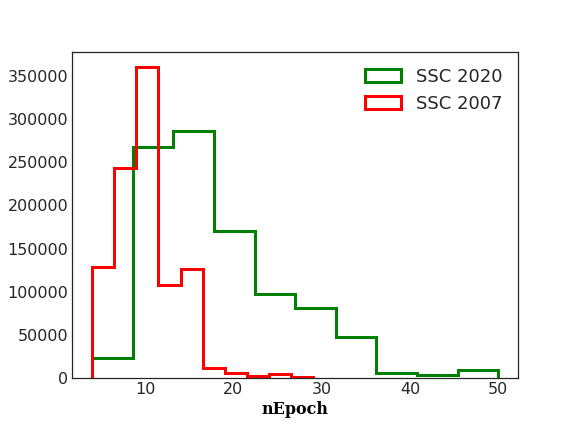
\includegraphics[width=0.4\textwidth, keepaspectratio]{figures/nepoch_compOvsN.png}
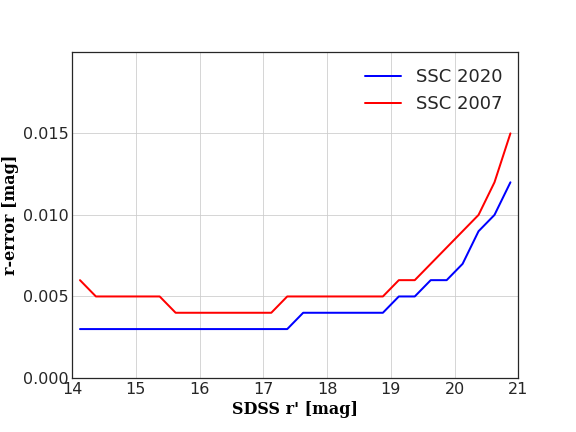
\includegraphics[width=0.4\textwidth, keepaspectratio]{figures/rerr_compOvsN.png}
\caption{{\it Left:} A comparison of the number of observational epochs for matched stars in the 2020 versus 2007 Standard Star Catalog (SSC). {\it Right:} A comparison of the median formal $r$ band photometric uncertainties of matched objects in the 2020 versus 2007 SSC, as a function of their mean $r$ magnitudes.
\label{fig:rerr_nvso}}
\end{figure}


\subsection{The derivation of  photometric zeropoint corrections using Gaia DR2 data\label{sec:GaiaCorr}} 

The variation of photometric zeropoints with position on the sky in the \pOc\ (see their eq.~4) was 
constrained using a combination of stellar colors \citep[the principal axes in color-color diagrams, for details 
see][]{2004AN....325..583I} and a standard star network \citep{2002AJ....123.2121S,2006AN....327..821T}. 
It is likely that residual errors in zeropoint calibration (e.g., a saw-tooth pattern, as a function of Declination,
was reported by \citealt{2013A&A...552A.124B}; see their Fig.~23) can be further minimized using 
uniformly calibrated space-based photometry from Gaia Data Release 2 (DR2). 

\subsubsection{Positional matching of the SDSS and Gaia catalogs}
Naively, one would positionally match the SDSS and Gaia DR2 catalogs using a matching radius of 
about 0.3 arcsec because SDSS positions are accurate to better than 0.1 arcsec per coordinate (rms) 
for sources with $r < 20.5$ mag \citep{2003AJ....125.1559P}.  However, observational epochs are
sufficiently different that stellar proper motions need to be accounted for; indeed, we find a very 
strong correlation between the SDSS-Gaia positional differences and proper motions published in 
the Gaia DR2 catalog (see the left panel in  Figure~\ref{fig:GaiaRApm}). After accounting for proper
motions,  the positions agree at the level of $\sim28$ milliarcsec (robust\footnote{We use robust estimator 
of standard deviation computed as $\sigma_G = 0.741*(q_{75}-q_{25})$, where $q_{25}$ and $q_{75}$ are 
the 25\% and 75\% quantiles, and the normalization factor 0.741 assures that $\sigma_G$ is equal to 
standard deviation for normal (Gaussian) distribution.}
rms, per coordinate). The 
residual differences are dominated by systematic errors in SDSS astrometry because there is
no increase of this rms with magnitude (see the right panel in Figure~\ref{fig:GaiaRApm}), and
because the contribution of Gaia's astrometric measurement uncertainties is negligible. 
The implied SDSS astrometric accuracy of $\sim28$ milliarcsec is substantially better than 
``$<0.1$ arcsec reported by \cite{2003AJ....125.1559P}, but note that here we used 
positions ``averaged'' over typically $\sim20$ SDSS runs (see the left panel in Figure~\ref{fig:rerr_nvso}). 

\begin{figure}[th!]
\centering 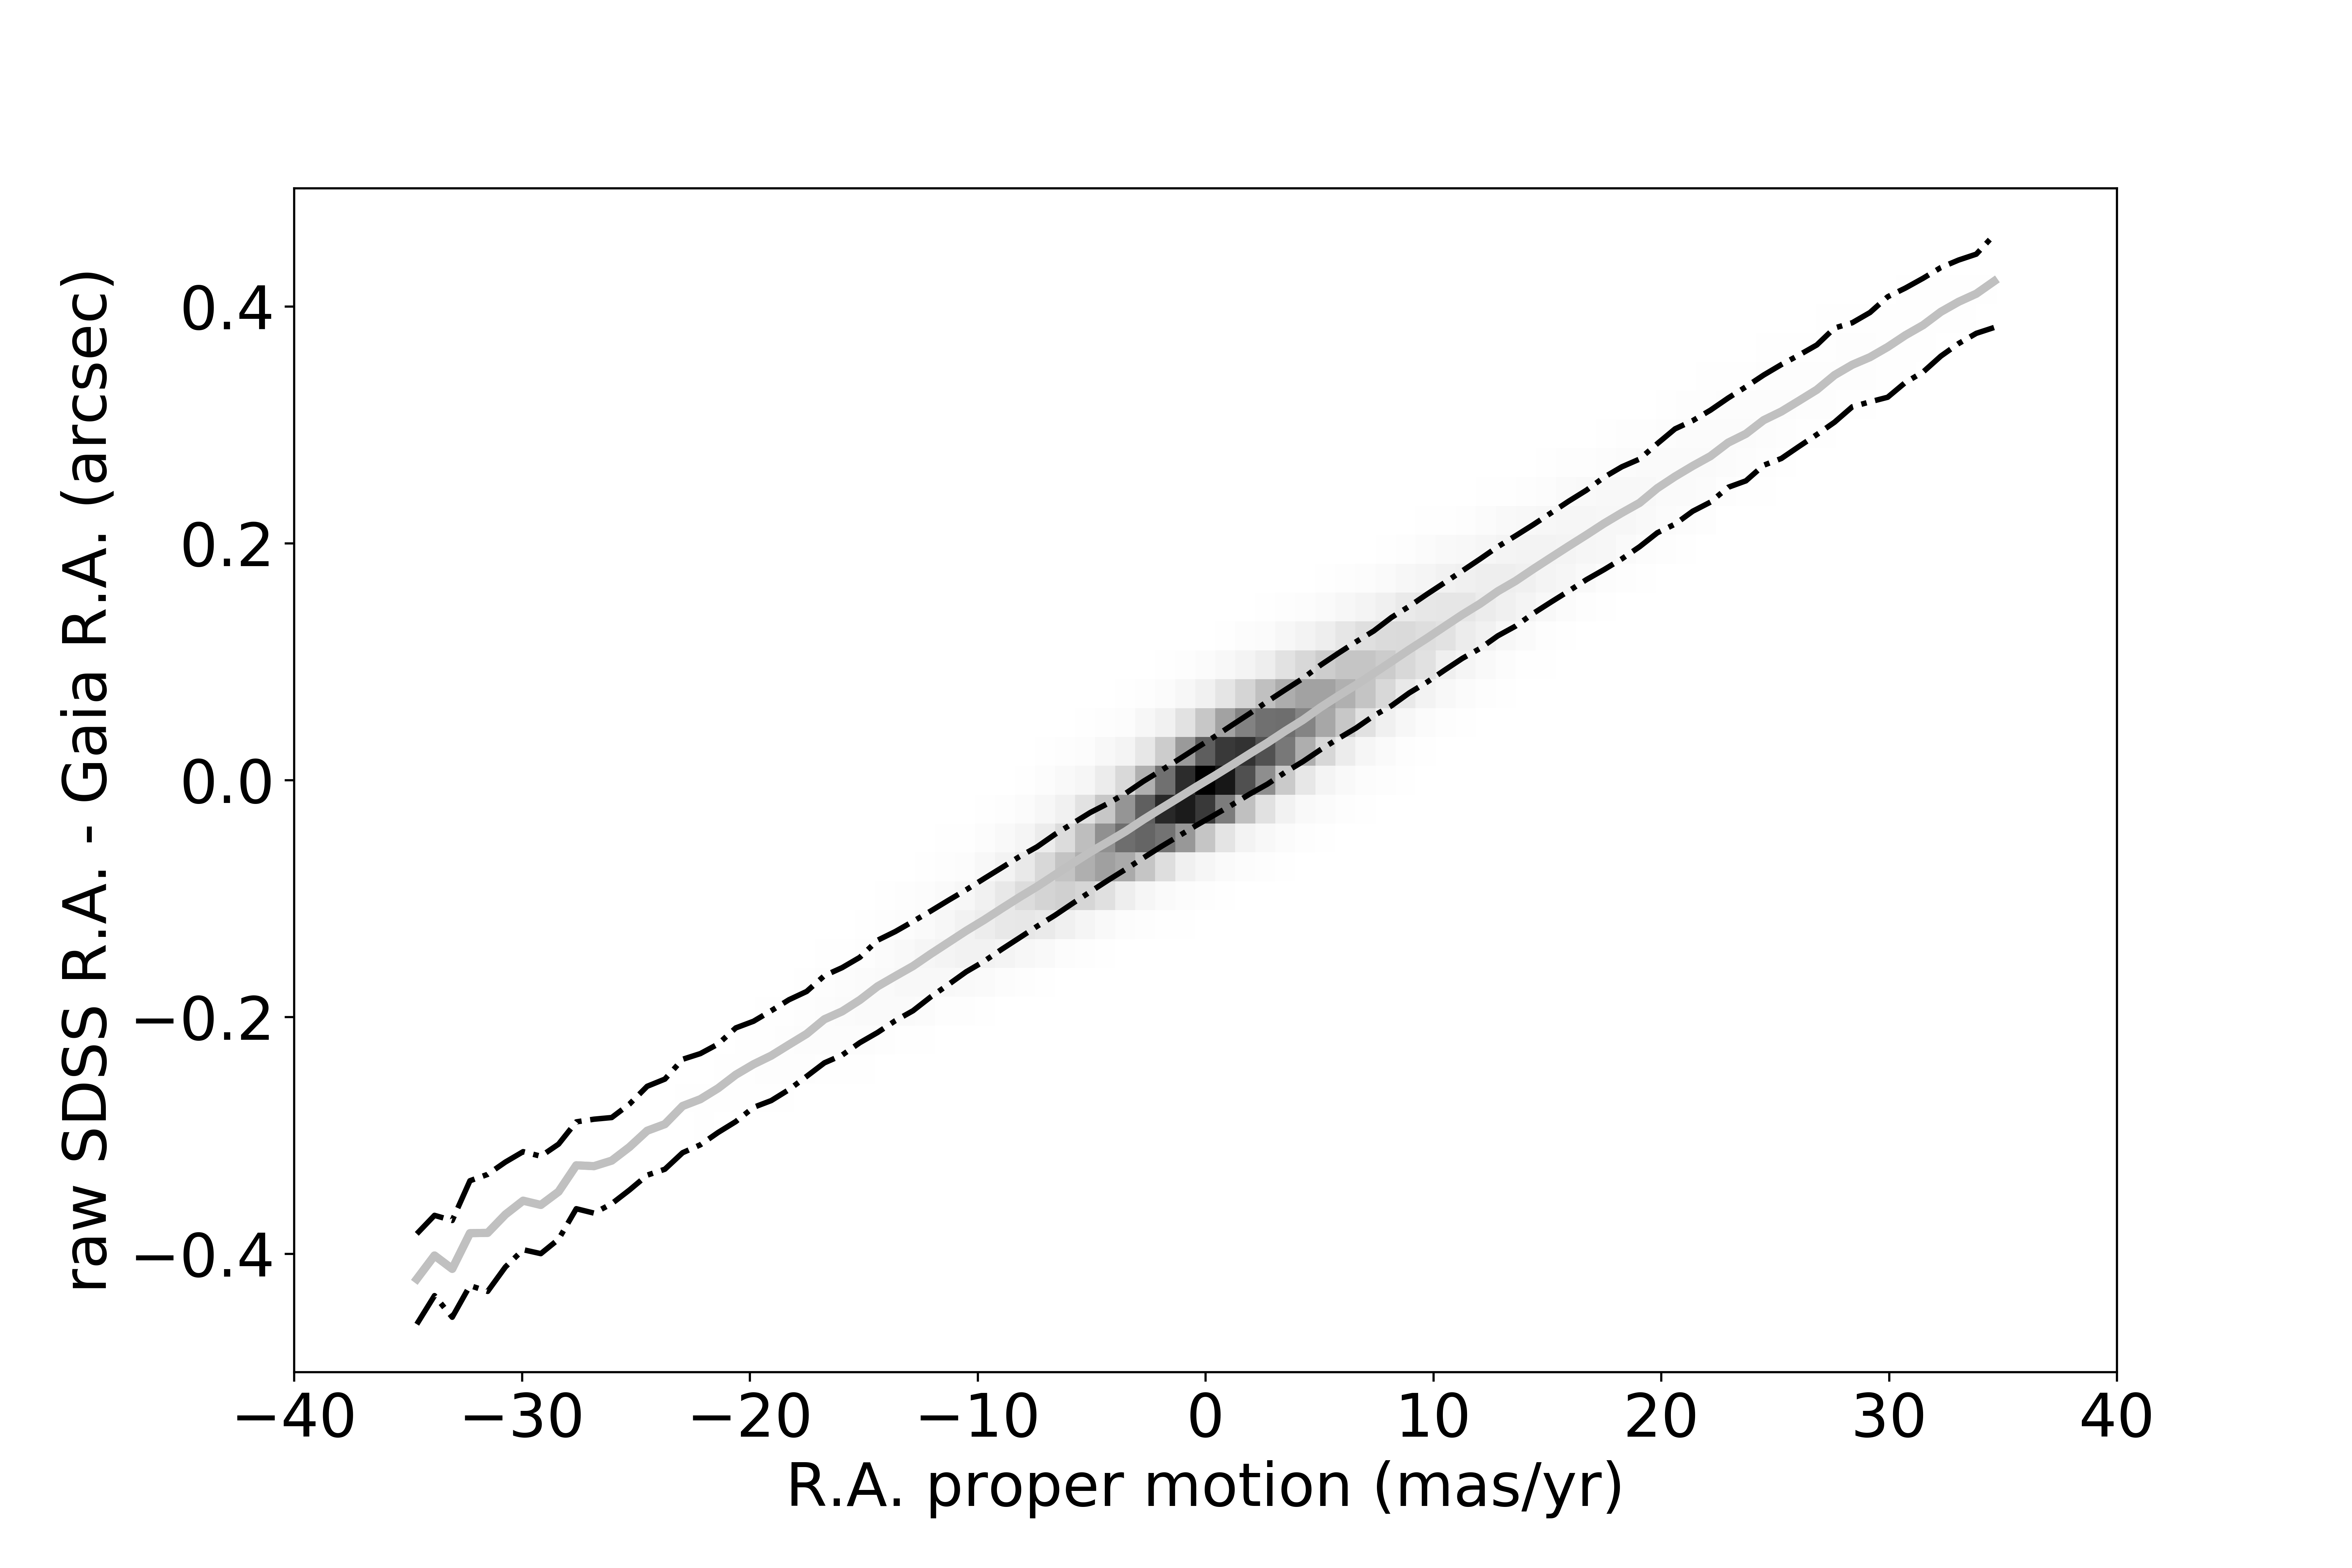
\includegraphics[width=0.4\textwidth, keepaspectratio]{figures/astroVSpm_RA_pm.png}
\centering 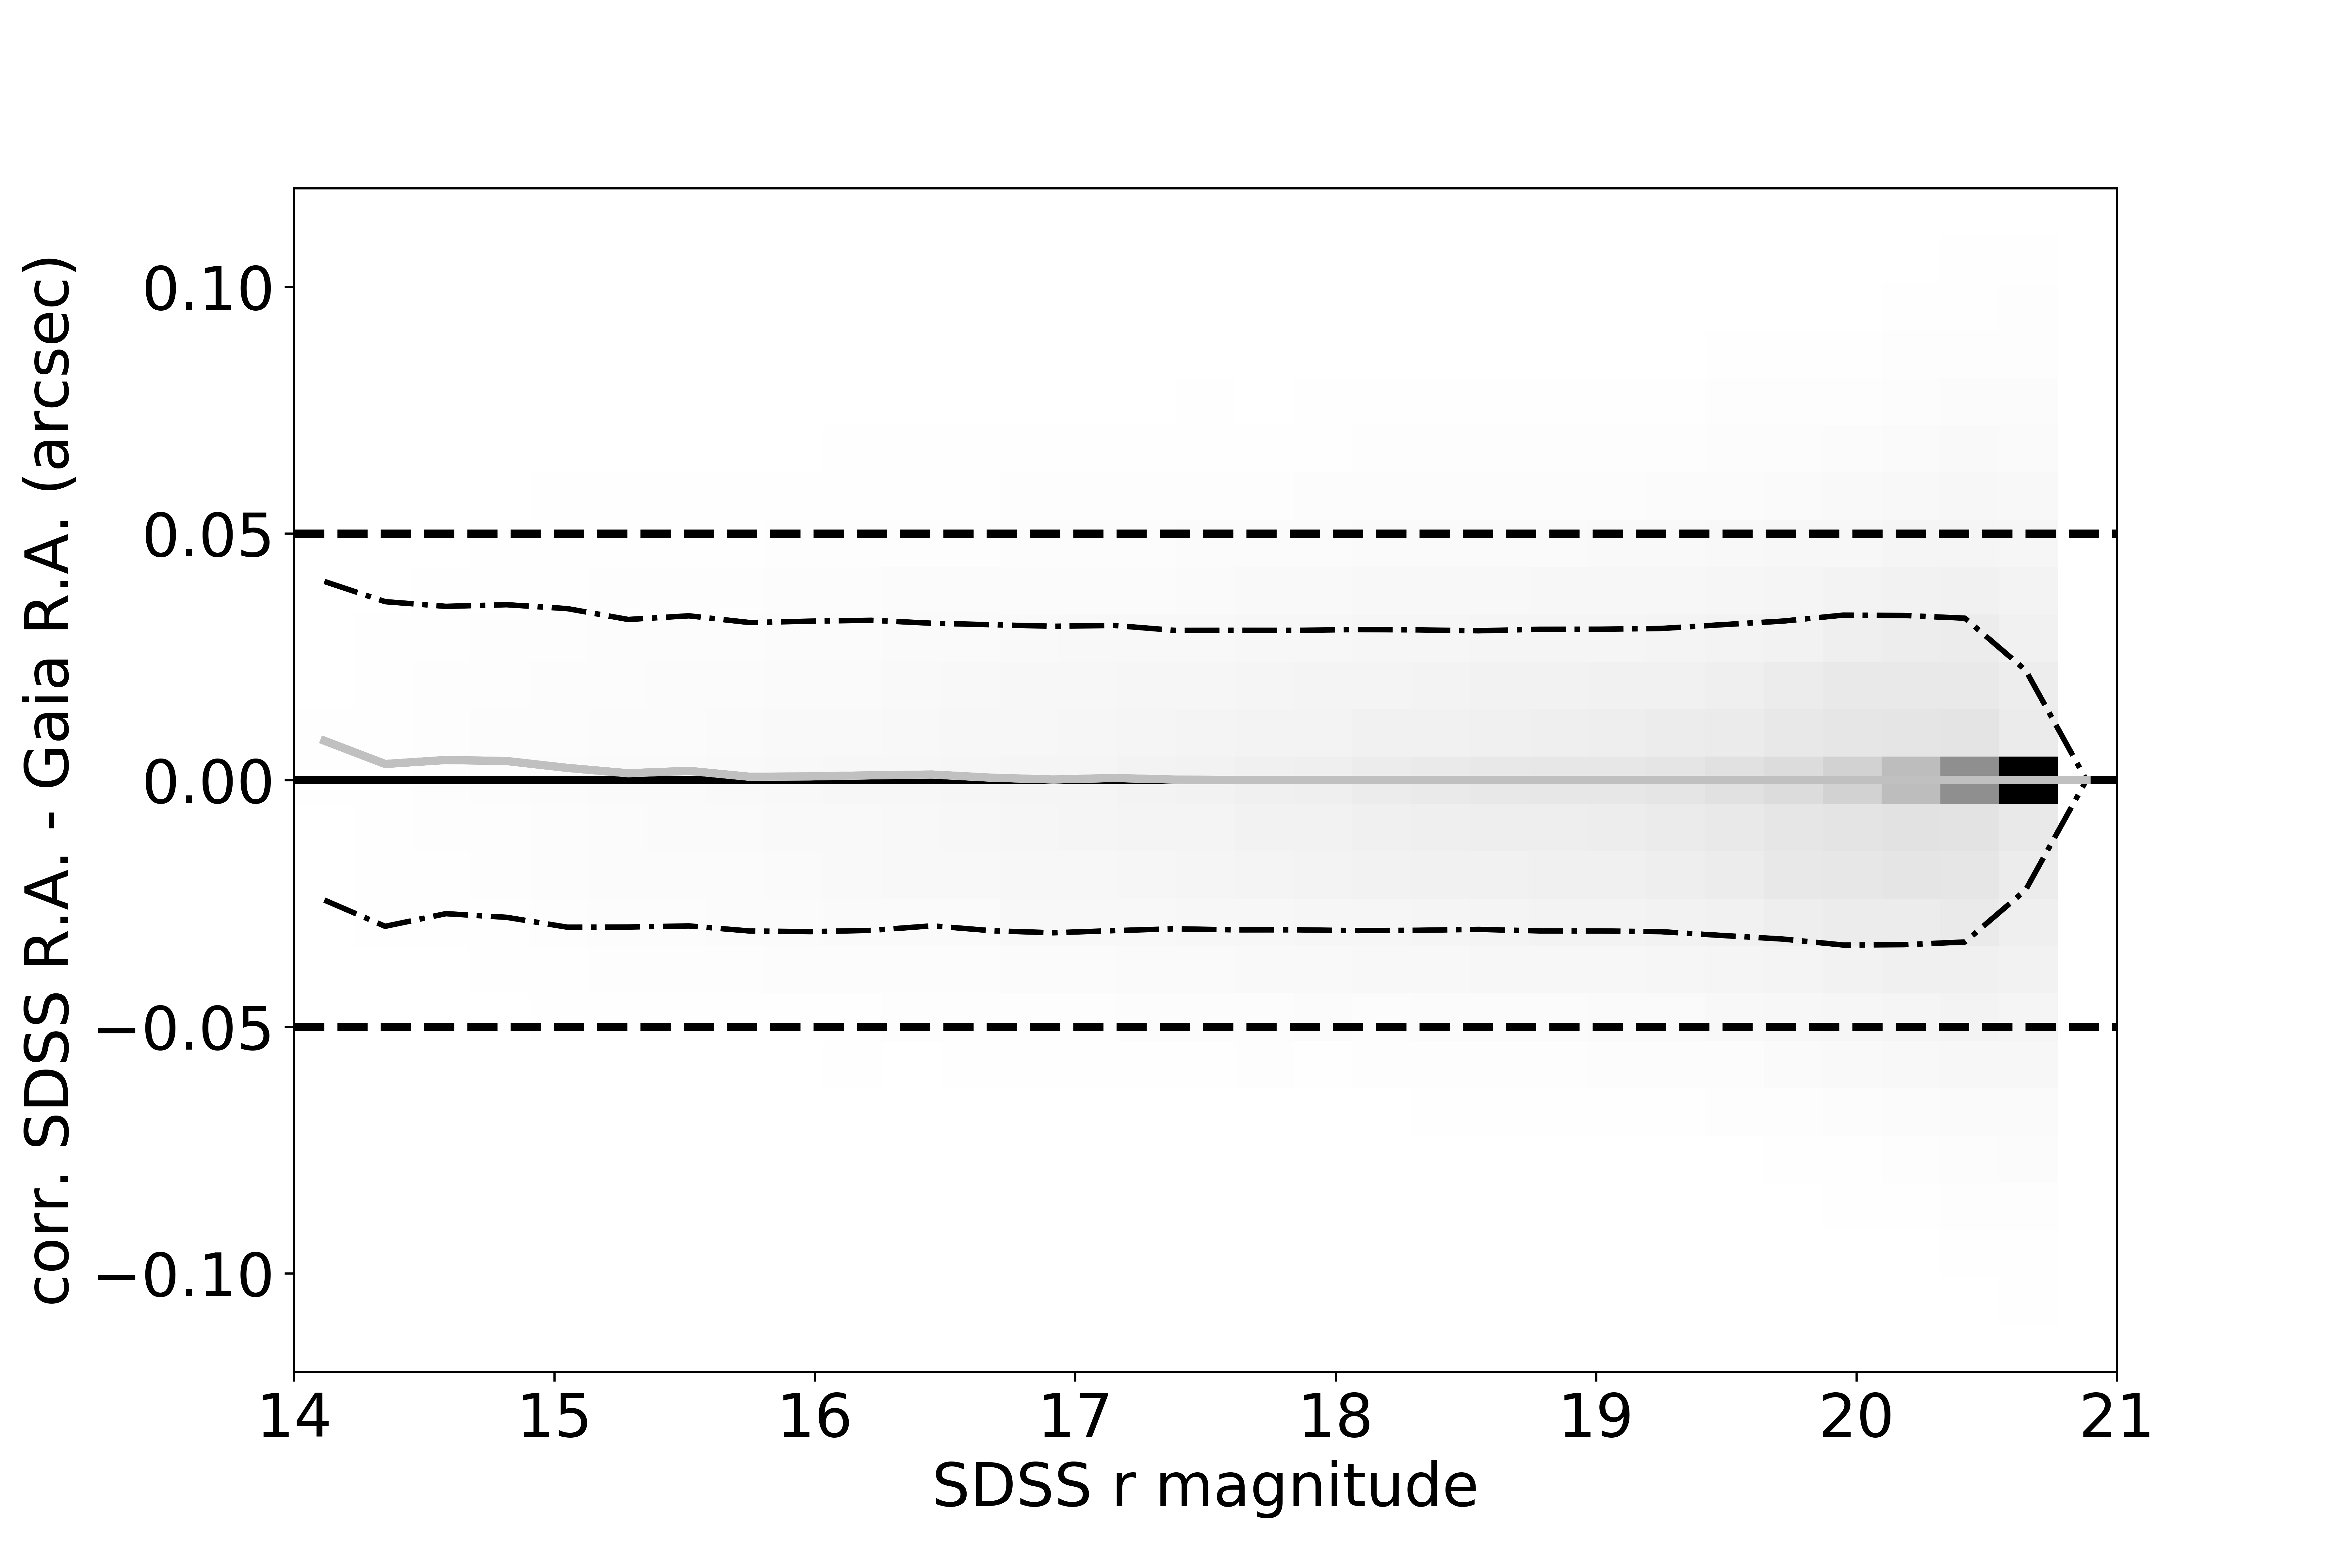
\includegraphics[width=0.4\textwidth, keepaspectratio]{figures/astroVSpm_RA_r.png}

\caption{The left panel shows the R.A. difference between SDSS and Gaia 
vs. R.A. proper motion reported by Gaia DR2. The solid line shows the median difference in bins 
of proper motion and the dashed lines mark the $\pm \sigma_G$ envelope around the medians,
where $\sigma_G$ is the robust standard deviation. The right panel shows the R.A. difference 
after correcting using the best-fit R.A. difference vs. 
proper motion curve, as a function of the SDSS $r$ magnitude. The residual differences are dominated 
by systematic errors in SDSS astrometry at the level of $\sim28$ milliarcsec (note that there is no increase with 
magnitude). Analogous plots for Declination quantities are similar. 
\label{fig:GaiaRApm}}
\end{figure}
  

\subsubsection{Gaia-based photometric zeropoint corrections}

Gaia DR2 reported Gmag magnitudes, which approximately span the SDSS $griz$ bandpasses, 
and BP and RP magnitudes, which approximately correspond to the blue and red halfs of the 
Gmag bandpass. We first used Gmag data to derive ``gray'' zeropoint corrections (applied to
all five SDSS bands), and then use the BP-RP color to derive zeropoint corrections for the 
$ugiz$ bands, relative to the $r$ band. 

The basic idea is simple: use Gaia's Gmag, Gmag$_{GaiaDR2}$, and the SDSS $gri$ magnitudes
to derive synthetic Gmag magnitudes based on SDSS data, Gmag$_{SDSS}$; bin the 
$\Delta$Gmag = (Gmag$_{SDSS}$-Gmag$_{GaiaDR2}$) residuals by R.A. and Dec, and 
use the median residuals per bin as the gray correction for SDSS photometry (as functions
of R.A. and Dec). Similarly, use Gaia's BP-RP color to derive synthetic $u-r$, $g-r$, $r-i$
and $r-z$ colors, and used the median residuals per bin as zeropoint corrections for 
the $ugiz$ bands. 

Given a large number of matched stars ($\sim 400,000$), and a large number of color combinations,
we do not attempt to derive analytic fits for synethtic magnitudes and colors but instead
use 0.05 mag narrow color bins and linear interpolation between the bins. We have verified
that even sixth-order polynomial fits do not provide better results than this simple 
numerical approach. An example of such a transformation is shown in Figure~\ref{fig:GrVSgi}. 


\begin{figure}[th!]
  \centering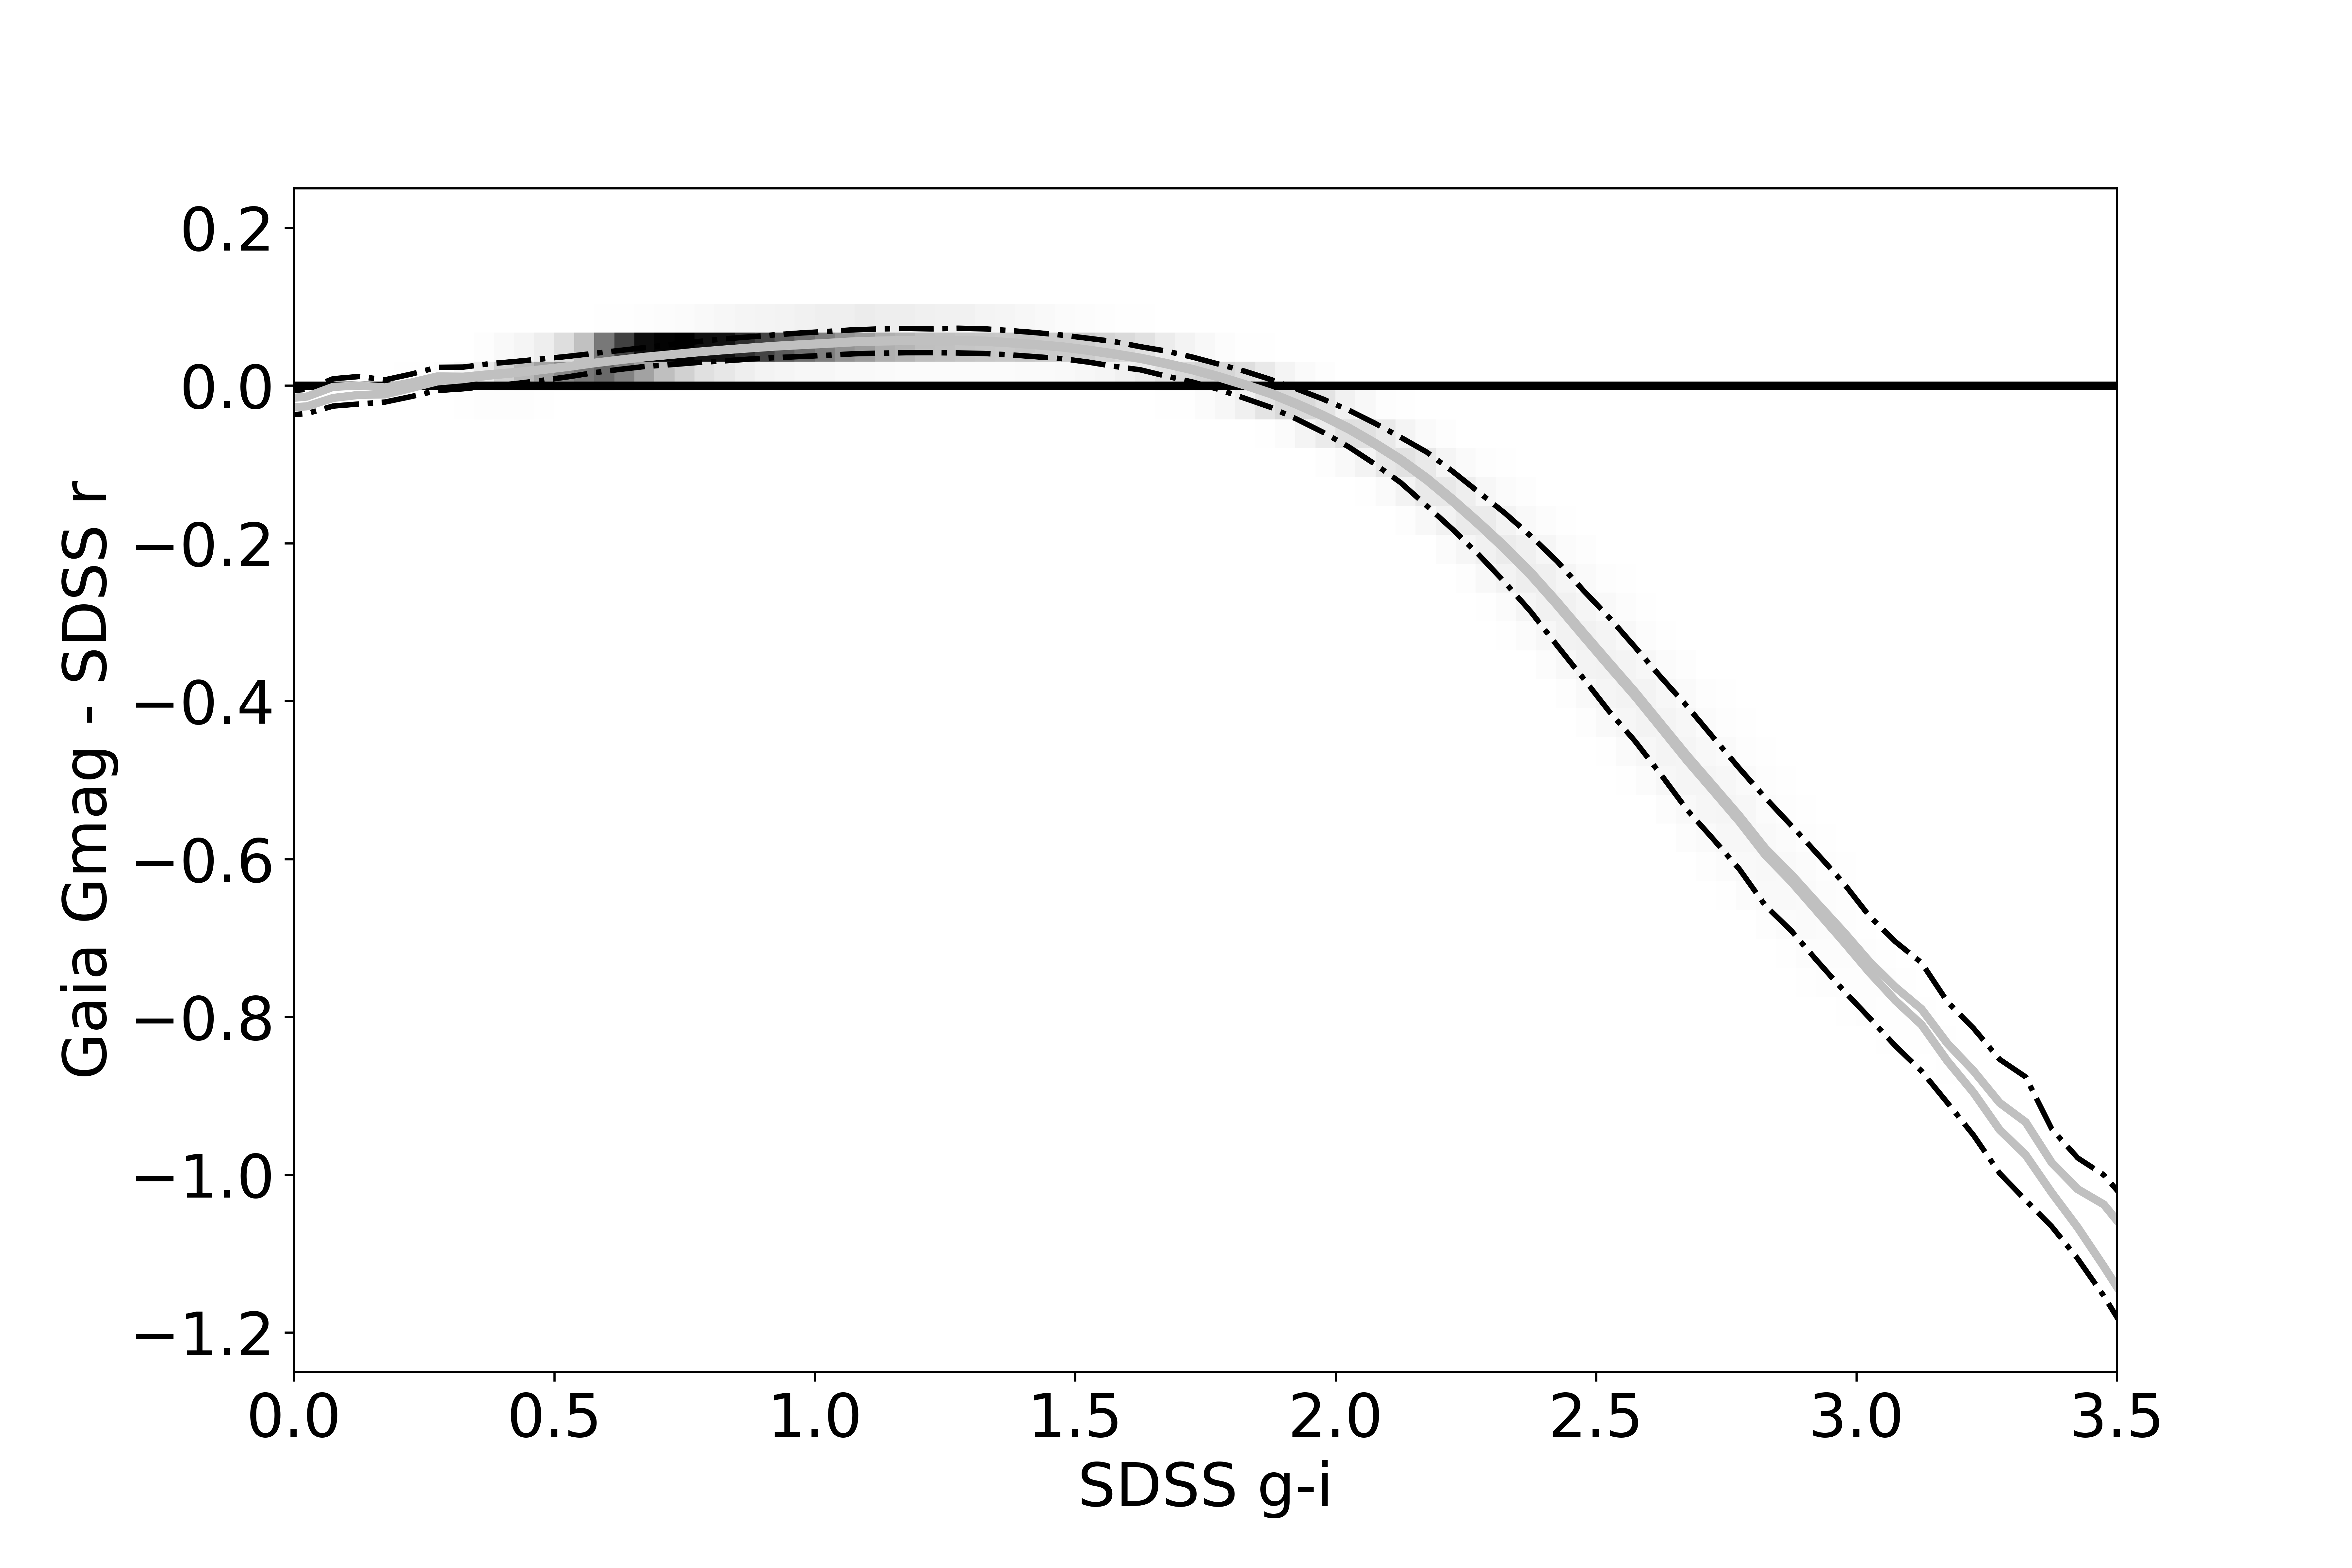
\includegraphics[width=8cm]{figures/GrVSgi.png} 
\caption{The variation of the difference between Gaia's Gmag magnitude from Data Release 2
and SDSS $r$ magnitude with the SDSS $g-i$ color.
The  color map illustrates the distribution of $\sim 393,000$ matched stars with 
$16<$Gmag$<19.5$. The two (barely distinguishable) solid lines represent the median 
values $\pm$ uncertainty of the median for 0.05 mag wide $g-i$ bins. The short-dashed 
lines show the median values $\pm$ the robust standard deviation for 
each bin. The horizontal solid line at zero is added to guide the eye. The mean of 
the two solid lines is used to derive the gray zeropoint correction, as a function of R.A.
and Declination.}
\label{fig:GrVSgi}
\end{figure}


The variation of Gmag residuals with Gmag (see Figure~\ref{fig:gaiaJump}) shows two 
interesting features. First, there is a sharp
``jump'' by about 3 millimag at Gmag$\sim$16.  This jump was a known (and 
larger problem) in Gaia Data Release 1, but appears not entirely fixed in DR2. The 
second ``feature'' is a large ($\sim0.01-0.02$ mag) discrepancy at the faint end:
about $\sim$10 millimag at Gmag=19.5 and $\sim$20 millimag at Gmag=20.5. 
A comparison of the SDSS catalog with Pan-STARRS and DES catalogs (see 
Section~\ref{sec:DESPS1} and Figure~\ref{fig:drVSr}) strongly suggests that the
origin of this discrepancy is a bias in Gaia's Gmag photometry at the faint end, rather 
than a problem with SDSS catalog (offsets between the SDSS and DES
photometry are $<1-2$ millimag at Gmag$\sim$20.5). 
 

\begin{figure}[th!]
    \centering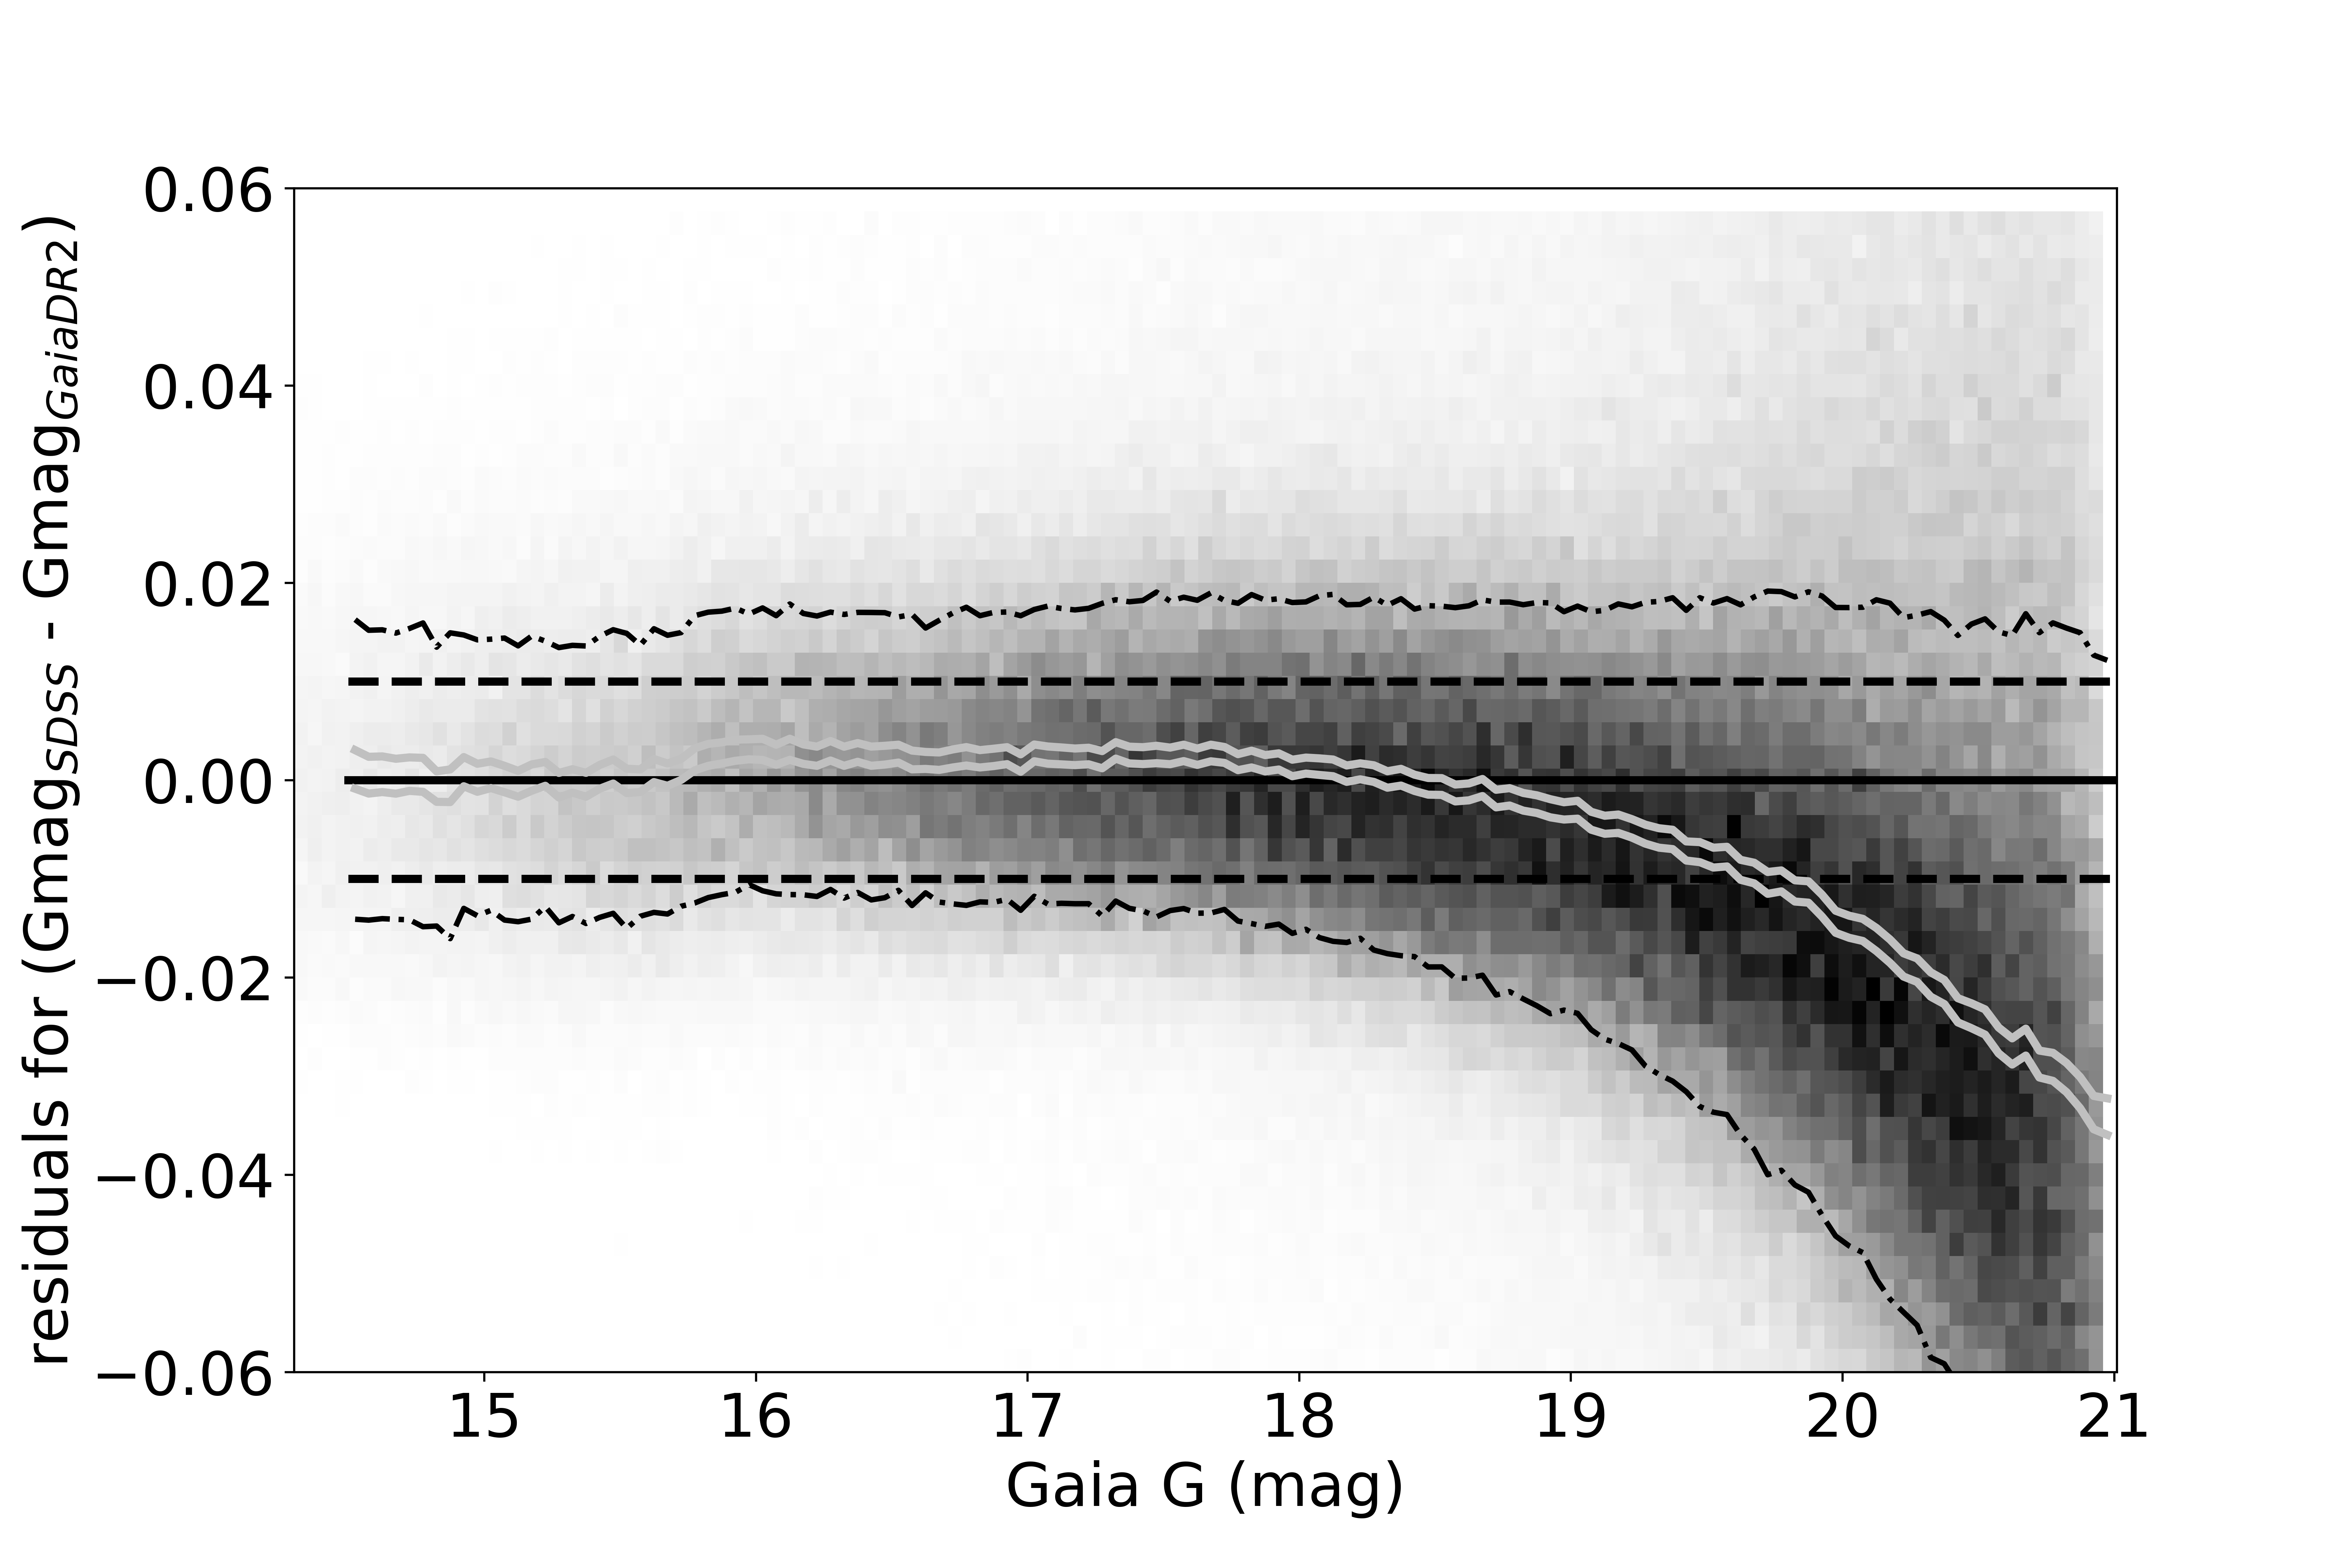
\includegraphics[width=9cm]{figures/GmagCorrectionTest_Gmag_Hess.png} 
\caption{The variation of the residuals between Gaia's Gmag from Data Release 2
and synthetic Gmag values generated using SDSS $gri$ photometry. The two solid 
lines represent the median values $\pm$ uncertainty of the median for each
0.05 mag wide Gmag bin. The short-dashed lines show the median values $\pm$ 
the robust standard deviation for each bin. The horizontal solid and long-dashed 
lines at zero and $\pm$0.01 mag, respectively, are added to guide the eye.
Note the jump by about 3 millimag at Gmag$\sim$16 -- this jump was a known and 
larger problem in Gaia Data Release 1, and apparently not entirely fixed in DR2. 
Note also large ($\sim0.01-0.02$ mag) discrepancy at the faint end -- a comparison 
of the SDSS catalog with Pan-STARRS and DES catalogs (see Figure~\ref{fig:drVSr}) 
suggests that its origin is a bias in Gaia's photometry at the faint end, rather than 
a problem with SDSS photometry.}
\label{fig:gaiaJump}
\end{figure}


Given these two features, we limit the calibration sample to the $16<$Gmag$<19.5$
magnitude range. We further restrict calibration stars to the $0.4 < g-i < 3.0$ color 
range (approximately A0 to M5 spectral range), yielding a sample of $\sim372,000$ stars. 
The behavior of median Gmag residuals per R.A. and Declination bin is shown in 
Figures~\ref{fig:graycorrRA} and \ref{fig:graycorrDec}. 


\begin{figure}[th!]
  \centering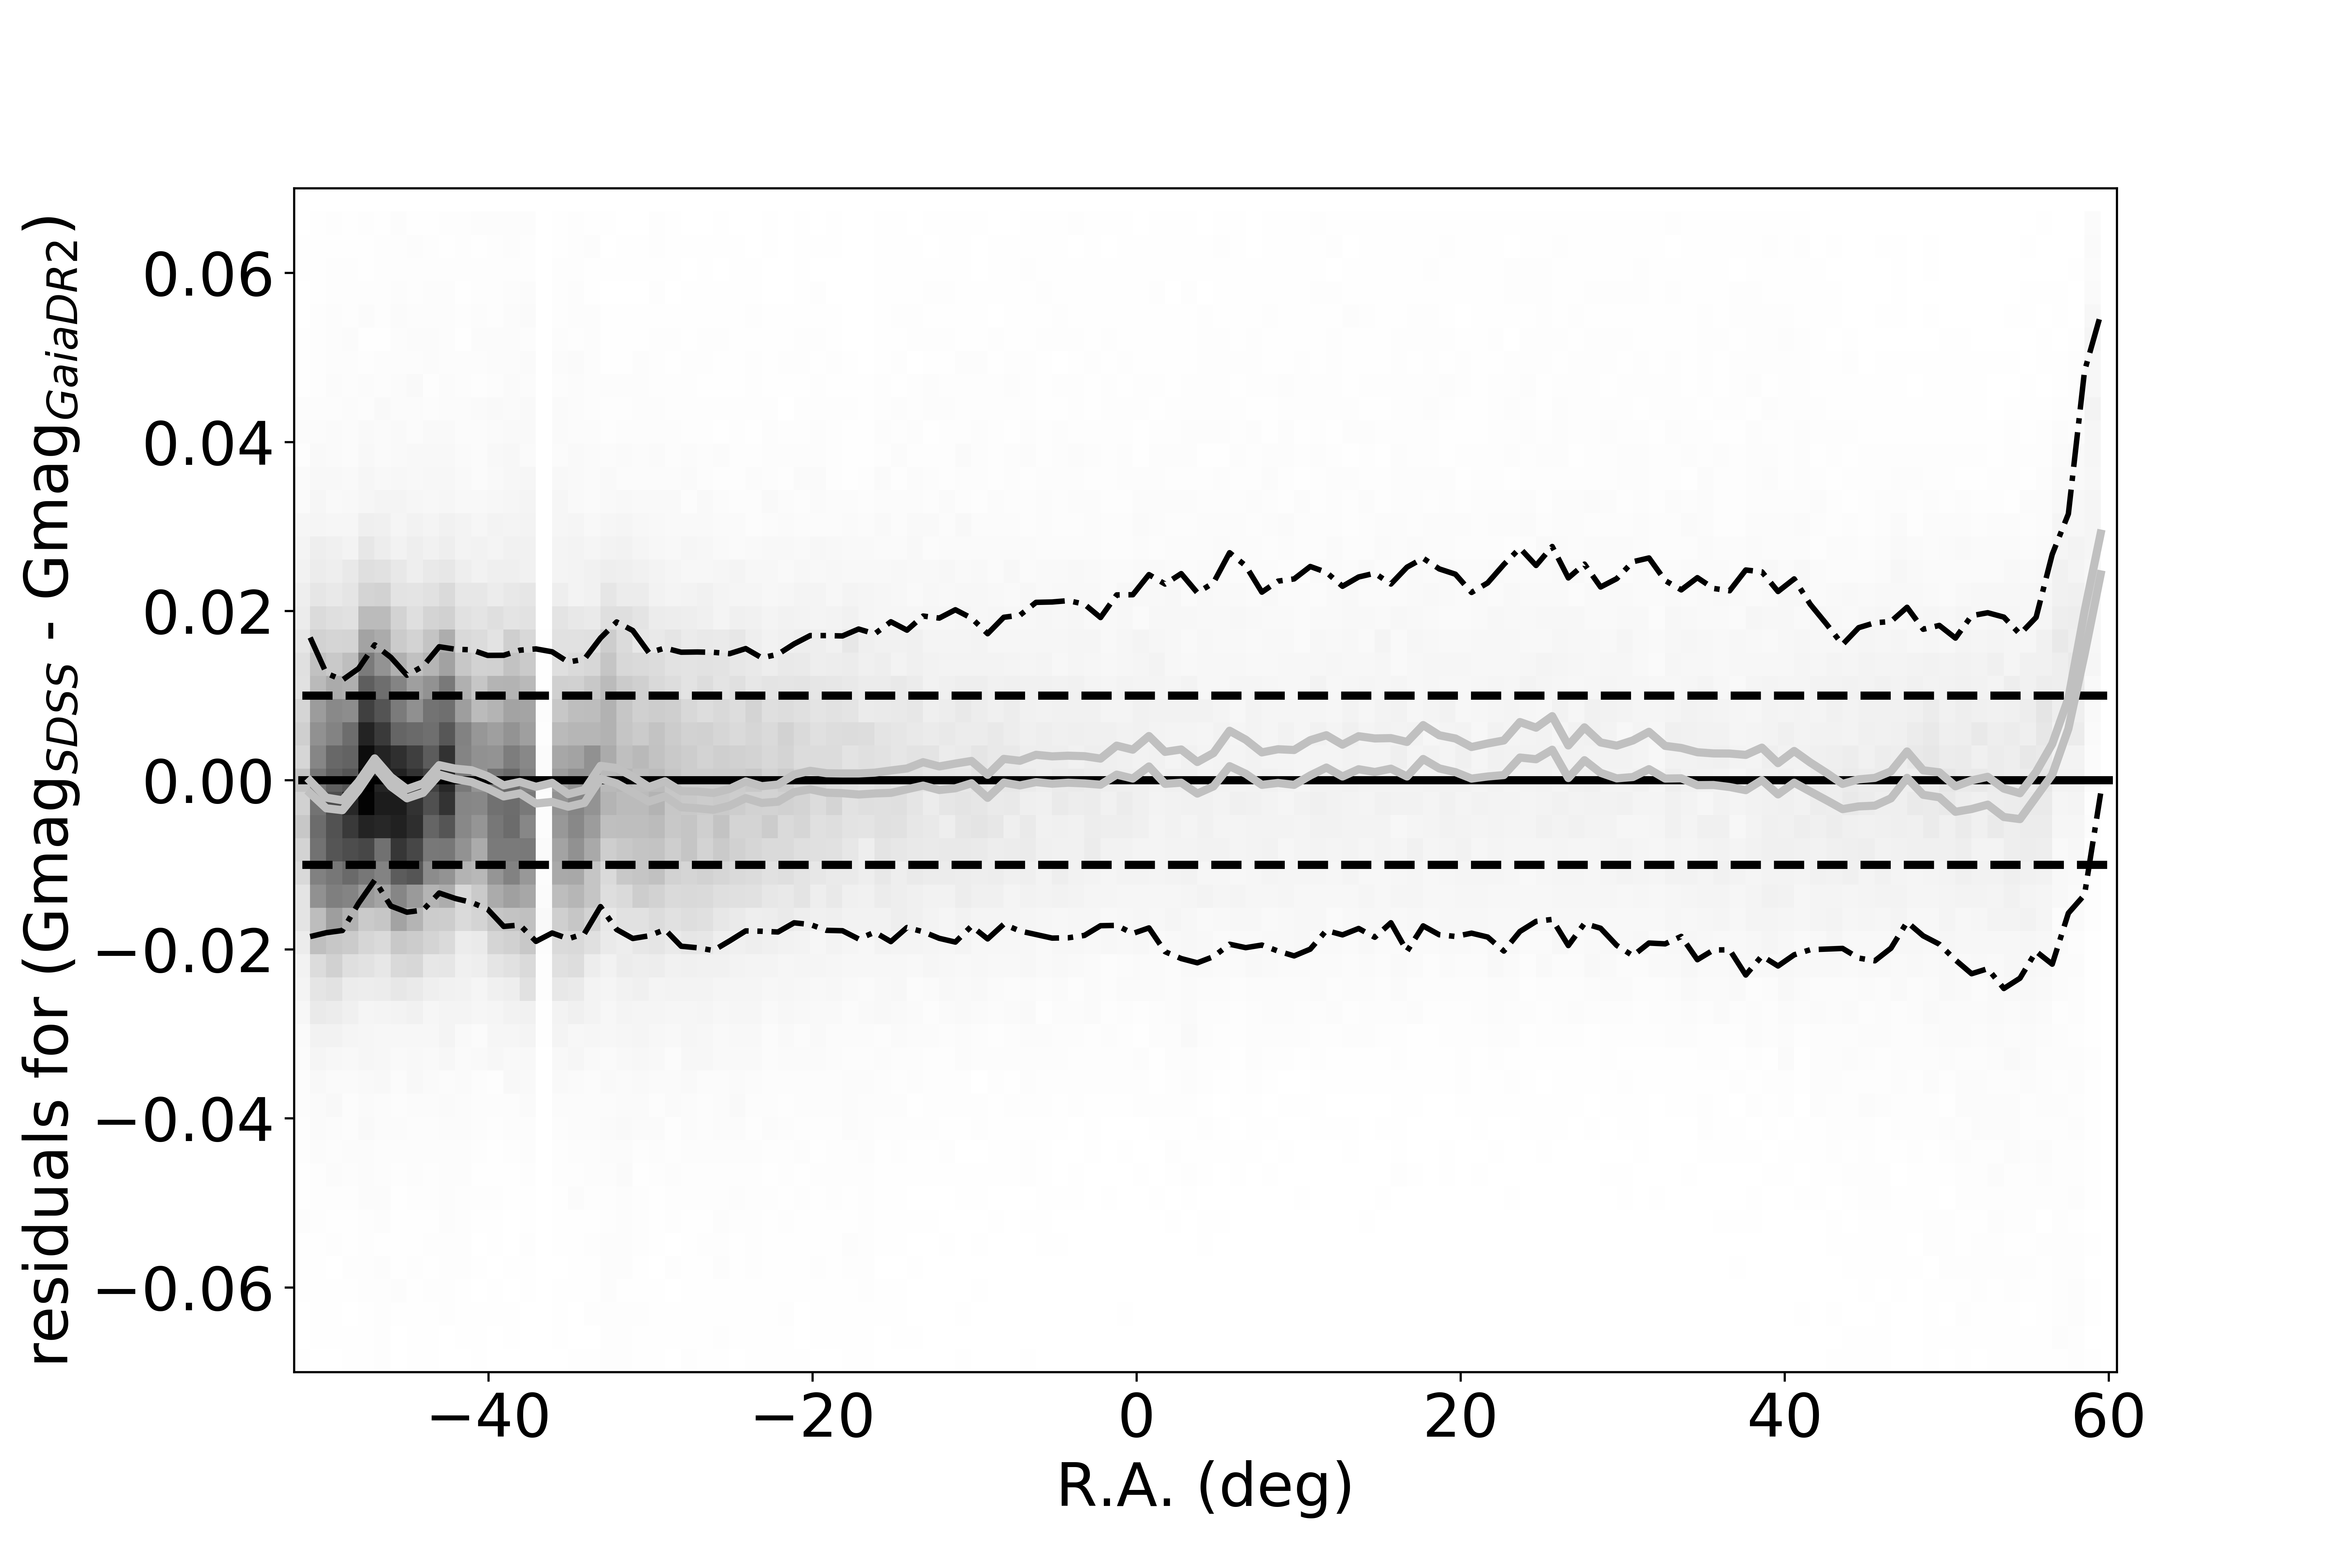
\includegraphics[width=8cm]{figures/GmagCorrection_RA_Hess.png} 
\caption{The R.A. variation of the residuals between Gaia's Gmag from DR2
and synthetic Gmag values generated using SDSS $gri$ photometry. The 
color map illustrates the distribution of $\sim 372,000$ matched stars with 
$16<$Gmag$<19.5$ and $0.4 < g-i < 3.0$. The two solid lines represent the 
median values $\pm$ uncertainty of the median for 1 degree wide R.A. bins. 
The short-dashed lines show the median values $\pm$ the robust standard 
deviation for each bin. The horizontal solid and long-dashed lines at zero and 
$\pm$0.01 mag, respectively, are added to guide the eye. The mean of the two 
solid lines is the gray correction, as a function of R.A., applied to the SDSS 
$ugriz$ magnitudes. The standard deviation for the applied correction is 3.5 millimag.}
\label{fig:graycorrRA}
\end{figure}

\begin{figure}[th!]
    \centering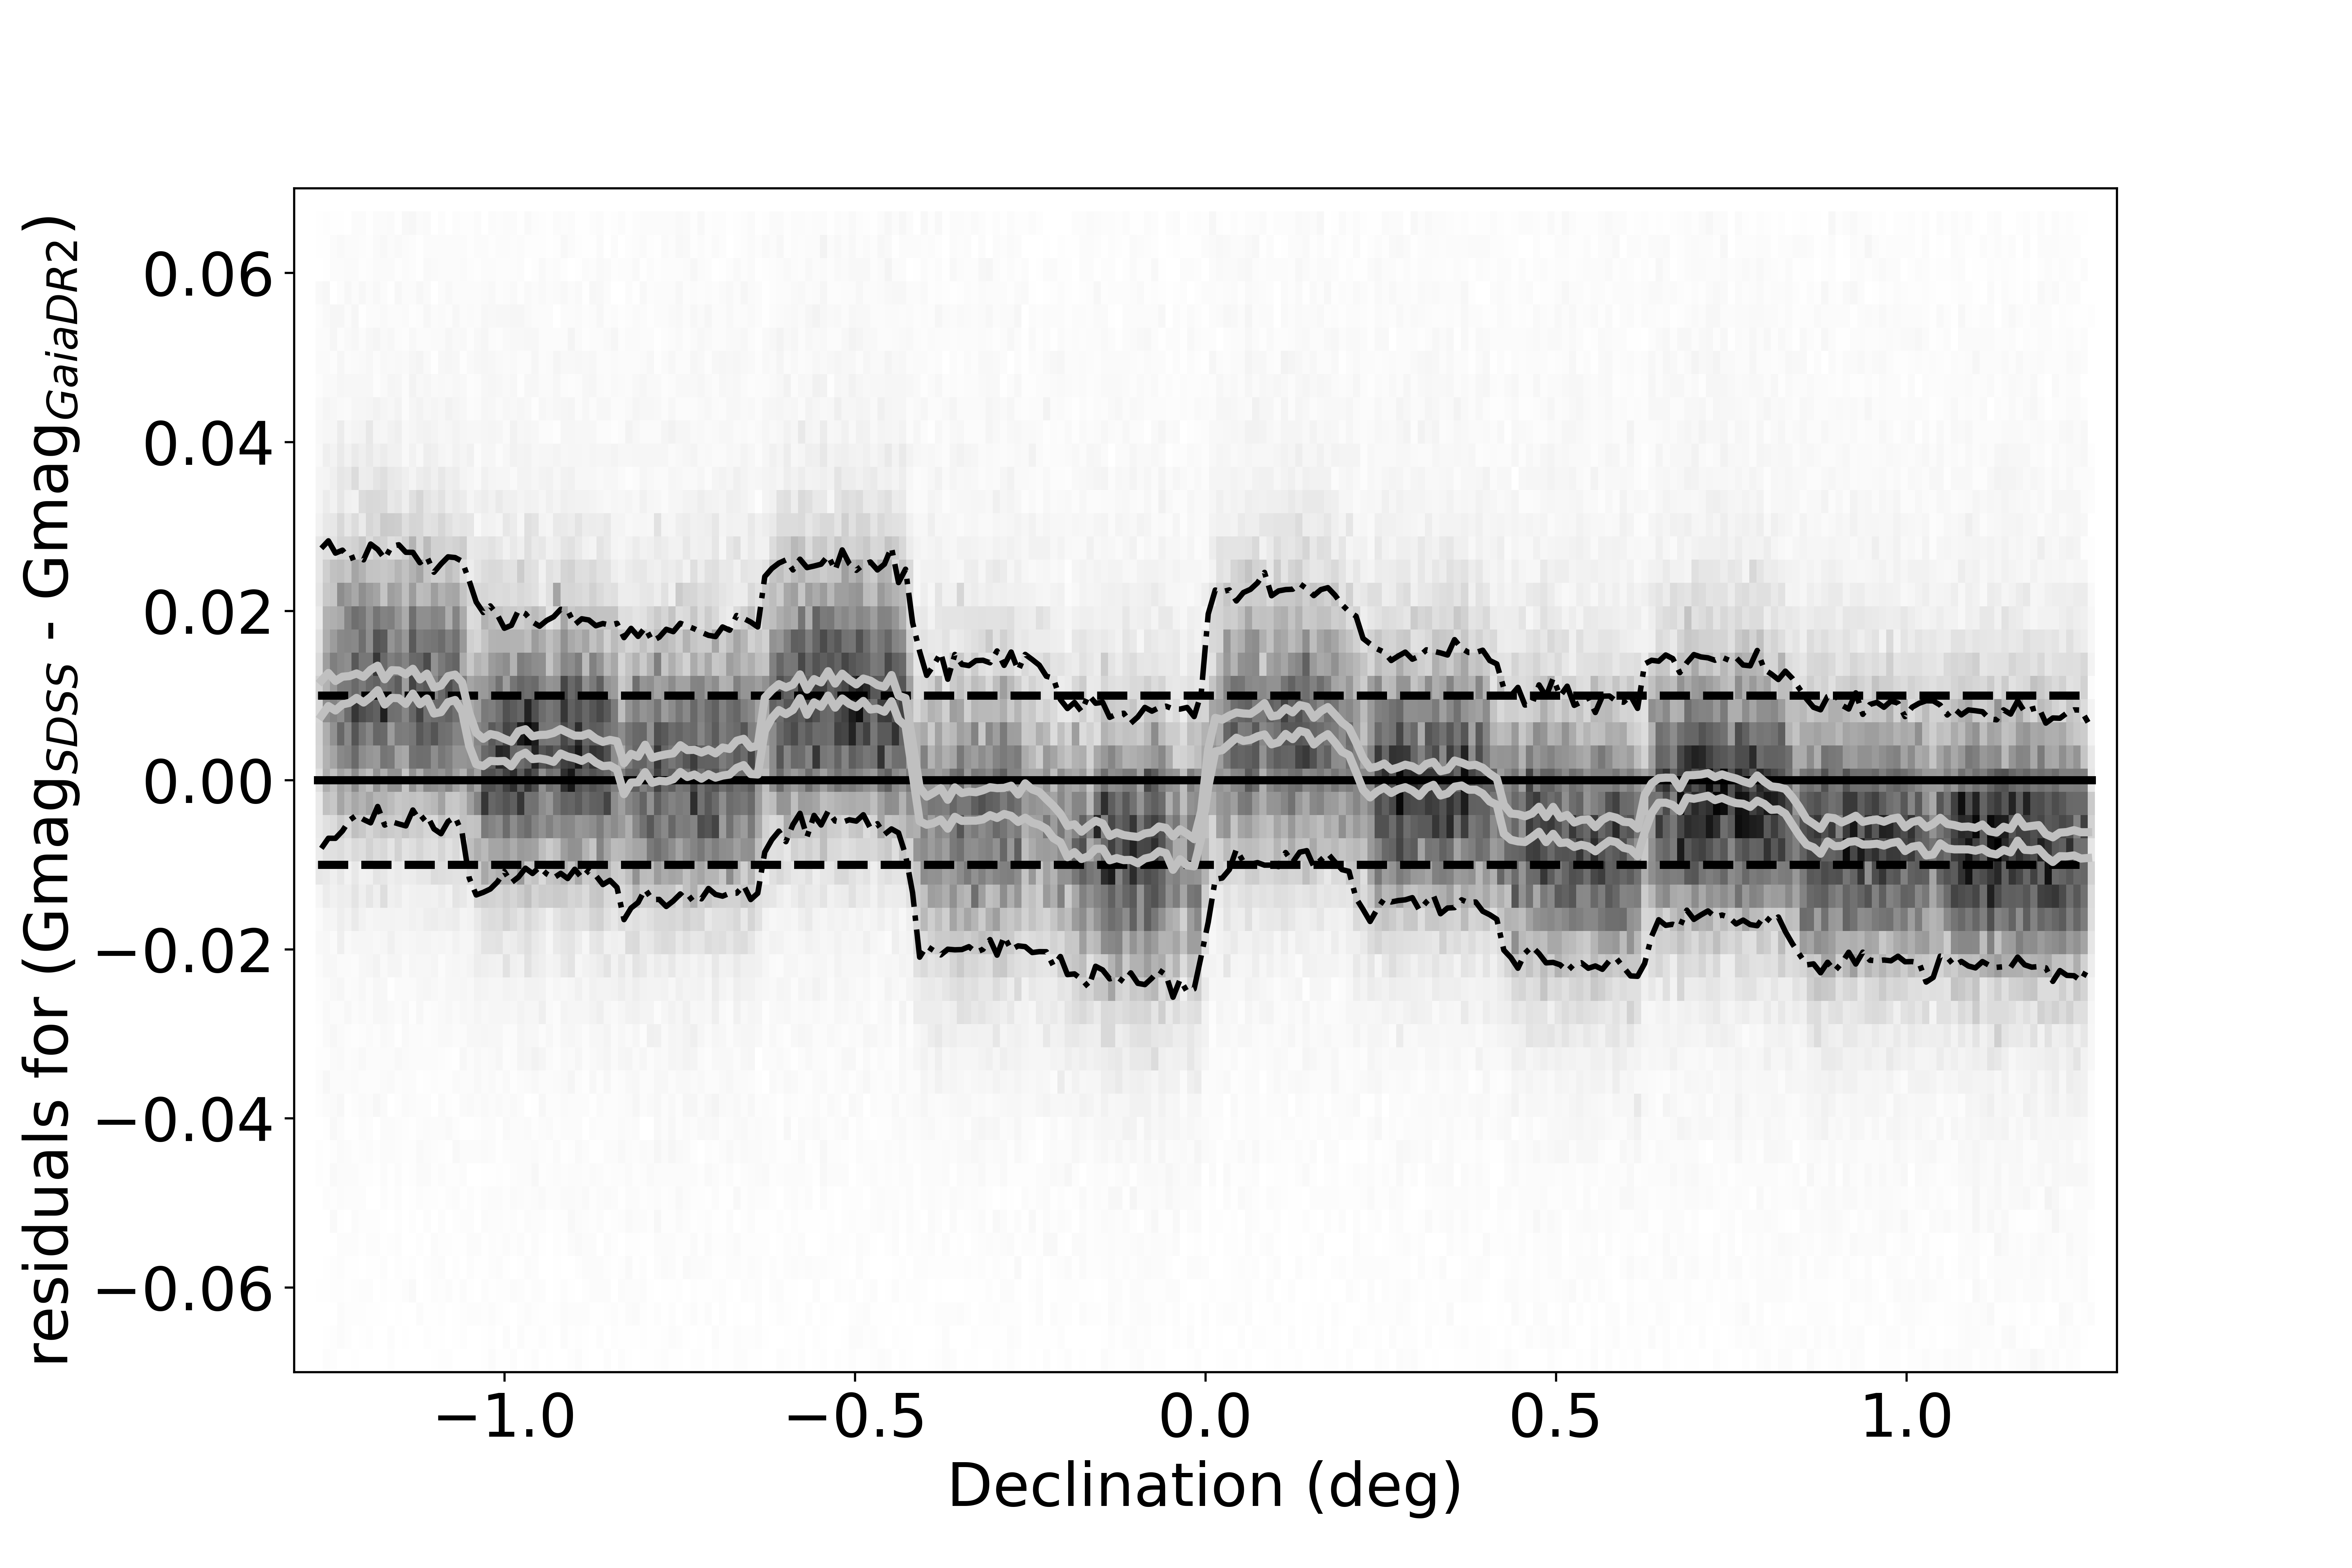
\includegraphics[width=9cm]{figures/GmagCorrection_Dec_Hess.png} 
\caption{Analogous to Figure~\ref{fig:graycorrRA}, except that here results are shown for
0.01 degree wide Declination bins. The 12 cleary visible regions correspond to
two SDSS scans (in R.A. direction) and six CCD columns in the SDSS camera. 
The standard deviation for the applied correction is 6.2 millimag, with a maximum
absolute value of $\sim0.01$ mag.}
\label{fig:graycorrDec}
\end{figure}


Except for a few degrees long region at the edge of Stripe 82 (R.A.$>$55 deg), the
SDSS photometric zeropoints are remarkably stable with respect to R.A.; the scatter
is only 3.5 millimag. On the other hand, there are clear deviations in Declination 
direction, which clearly map to the 12 scanning strips that fill Stripe 82. We note
that discrepancies never exceed 0.01 mag (with a scatter of 6.2 millimag), which was 
the claimed accuracy of the \pOc. Thanks to a large number of stars in the sample,
and well calibrated Gaia's photometric zeropoints across the sky, we can now 
constrain SDSS zeropoints with a precision of about 1 millimag per 0.01 degree
wide Declination bin. 

The residuals shown in Figures~\ref{fig:graycorrRA} and \ref{fig:graycorrDec} are
applied as ``gray'' zeropoint corrections to $ugriz$ magnitudes, as functions of 
R.A. and Declination, to all 991,472 stars in the catalog. This catalog version was
labeled v3.1, and it is publicly available\footnote{See http://faculty.washington.edu/ivezic/sdss/catalogs/stripe82.html}. 

In the next re-calibration step, we derive synthetic $u-r$, $g-r$, $r-i$ and $r-z$ colors
from Gaia's BP-RP color, using the same binning procedure as we used above for 
Gmag$-r$ vs. $g-i$ variation (see Figure~\ref{fig:GrVSgi}). An example of color residuals 
is shown in Figure~\ref{fig:riresid}.  The median residuals per R.A. and Declination bins 
are then used as zeropoint corrections for the $ugiz$ bands. We required that the median
offsets for all stars are vanishing and thus photometry in the new catalog is on the 
same AB scale as the old catalog (for related discussion, see Section~\ref{sec:AB}). 
The robust standard deviation for all zeropoint corrections is listed in Table~\ref{tab:GaiaRMS}. 

\begin{deluxetable}{l|c|c}[ht!]
\tablecaption{The robust standard deviation for binned SDSS-based vs. Gaia-based color residuals$^a$. \label{tab:GaiaRMS}}
\tablehead{
\colhead{Color } & \colhead{rms for R.A.} & \colhead{rms for Dec}
}
\startdata
 gray (Gmag) &    3.5         &    6.2   \\
    $u-r$        &   0.0$^b$  &   20.4   \\     
    $g-r$        &   4.0         &    4.2    \\
    $r-i$         &   4.1         &    3.2    \\ 
    $r-z$        &   7.4         &    2.9    \\ 
\enddata
\tablenotetext{a}{The standard deviation for applied Gaia-based zeropoint corrections. The robust standard deviation 
is estimated using interquartile range. The units are millimag.} 
\tablenotetext{b}{For the $u$ band, we could not confirm the R.A. behavior of Gaia-based zeropoint correction 
with the CFIS data and didn't apply it. The large $u$ band correction as a function of Declination was validated 
with the CFIS data (see Section~\ref{sec:CFIStest}).} 
\end{deluxetable}
 

\begin{figure}[th!]
    \centering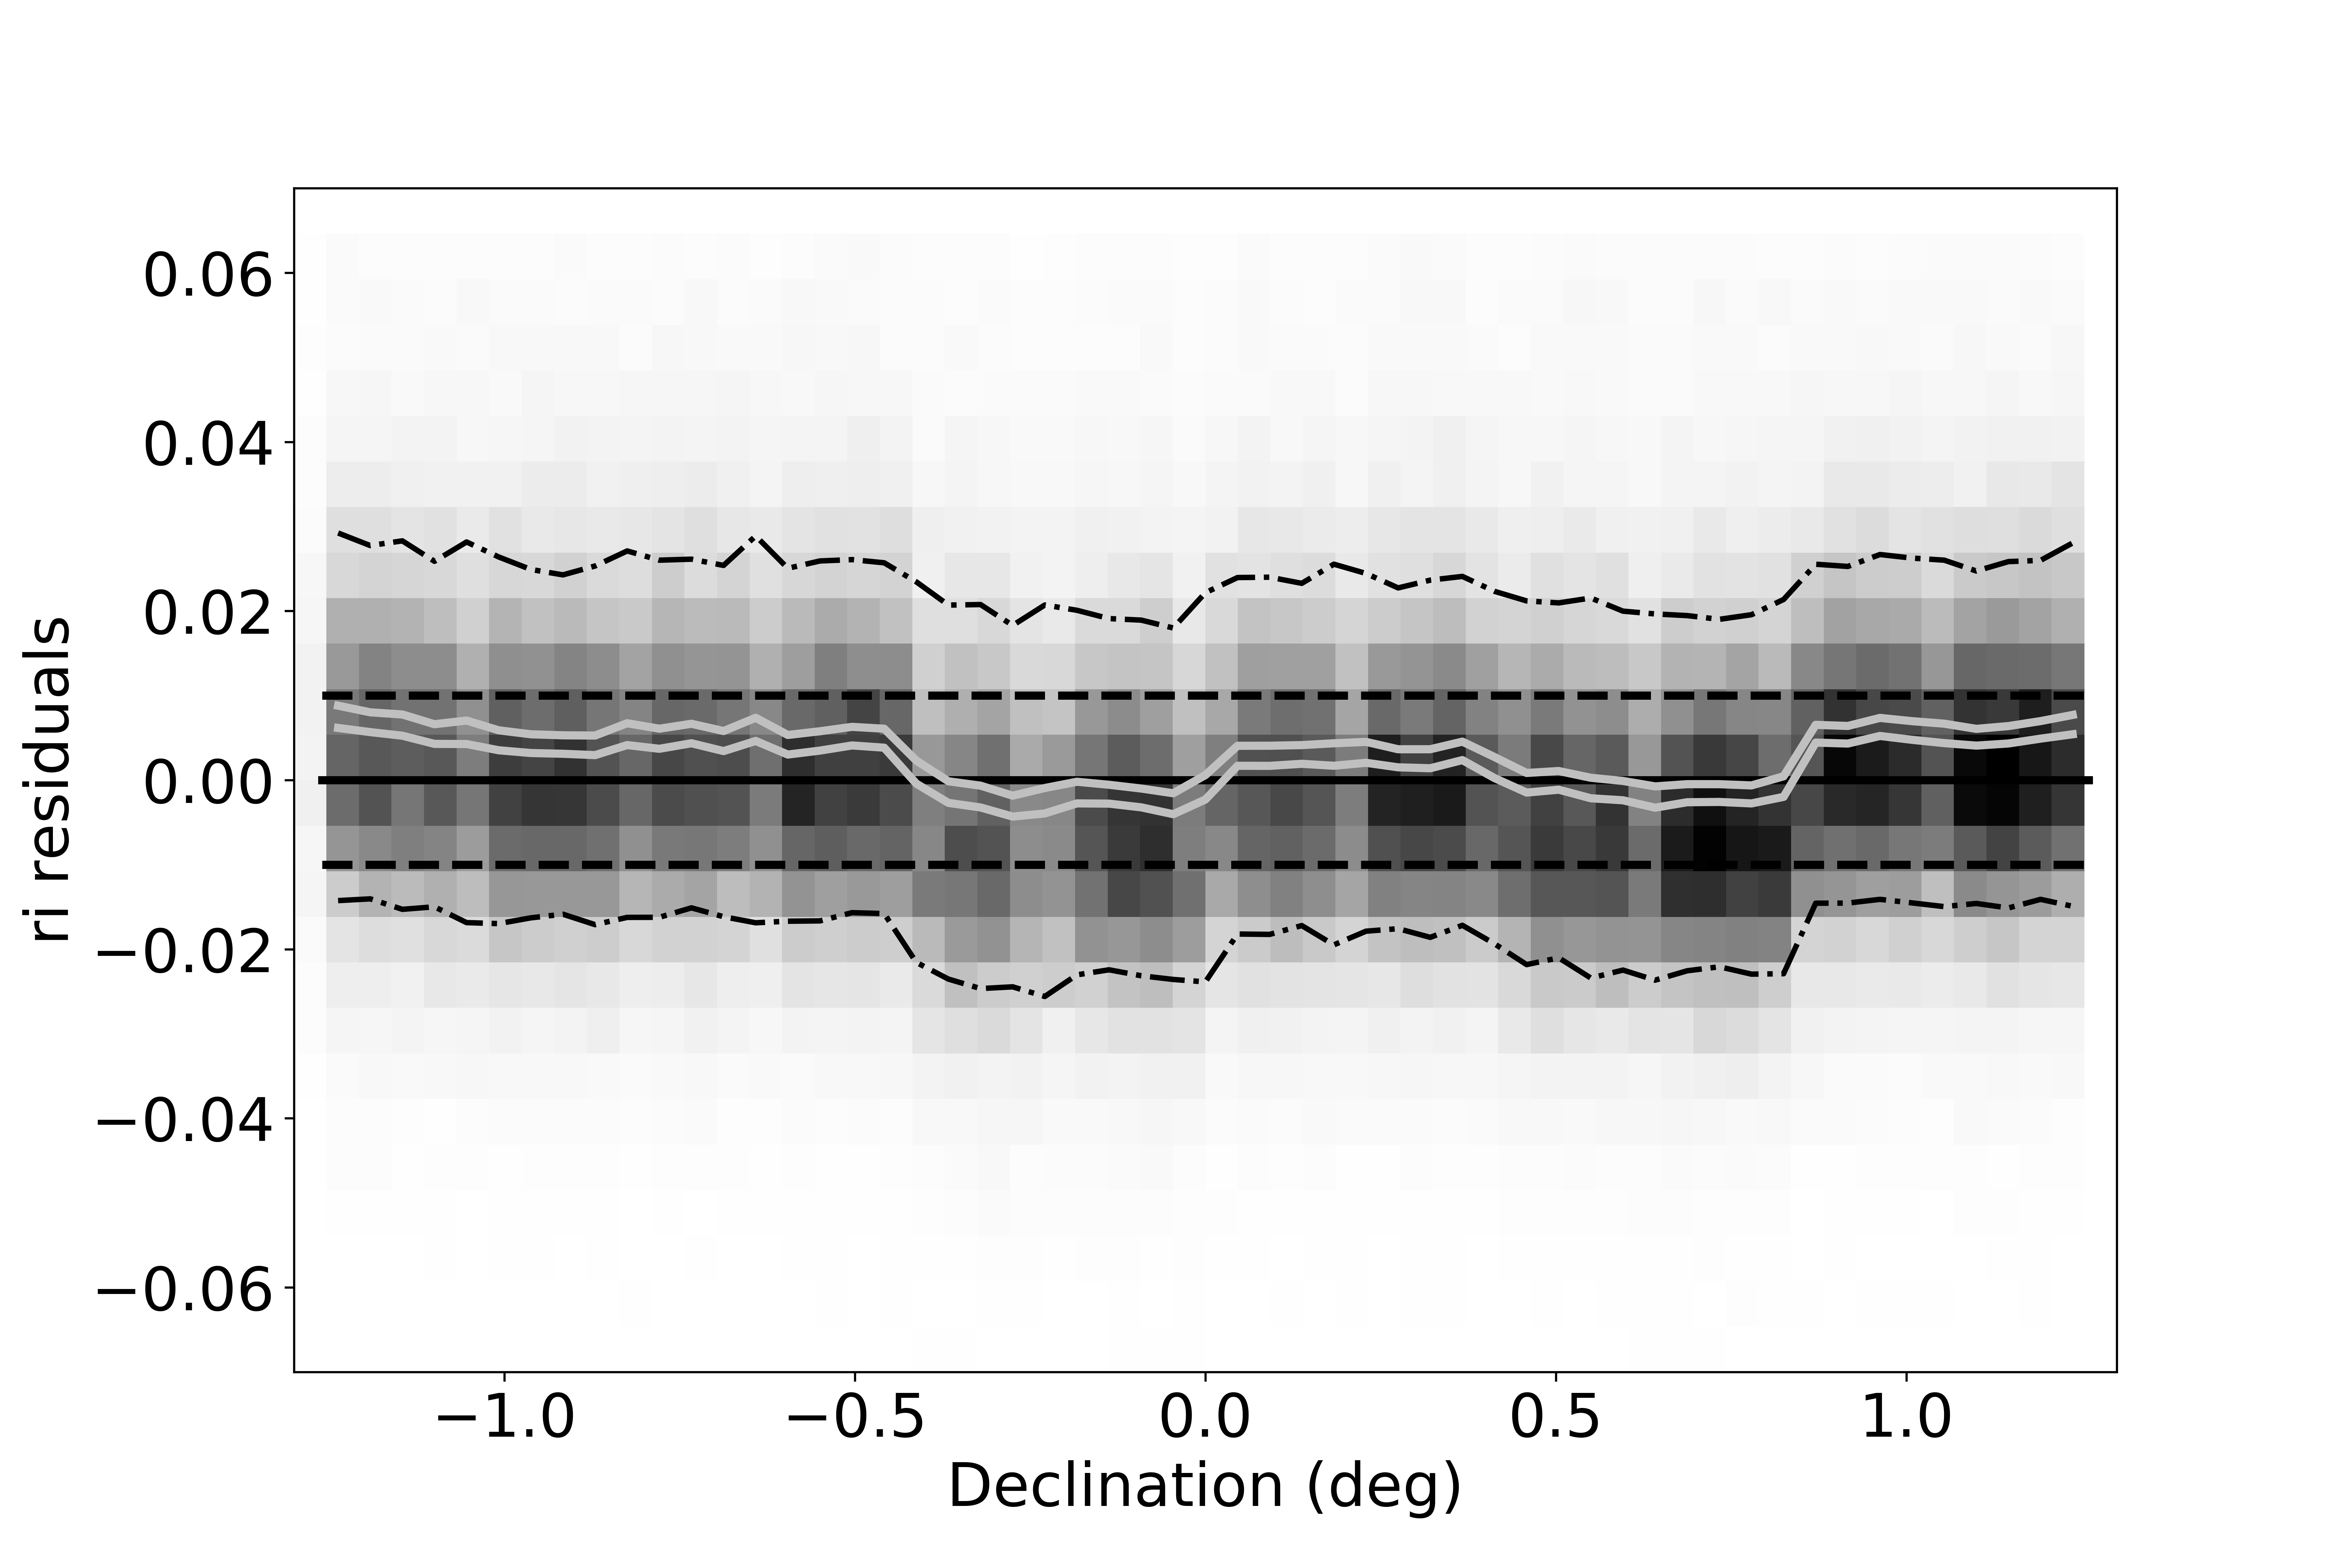
\includegraphics[width=9cm]{figures/colorResidGaiaColorsB_ri_Dec_Hess.png} 
\caption{Analogous to Figure~\ref{fig:graycorrDec}, except that here residuals 
correspond to differences between the SDSS $r-i$ color and a synthetic $r-i$ color
generated using Gaia's $BP-RP$ color. Note the signature of SDSS camera columns
at the level of a few millimags. The standard deviation for the binned medians is 
3.2 millimag (for other bands, please see Table~\ref{tab:GaiaRMS}.}
\label{fig:riresid}
\end{figure}


The largest corrections were derived for the $u$ band. Given that Gaia's BP-RP
color does not strongly constrain the $u$ band flux, we used the CFIS catalog 
(see Section~\ref{ssec:cfis}) as an independent verification test. We verified that
zeropoint errors in the SDSS catalog implied by Gaia's and CFIS data agree at the
level a few millimags in Declination direction, but found $\sim$0.01-0.02 mag
large inconsistencies for R.A. bins. For this reason, we only applied $u$ band 
correction in Declination direction. The plausible $u$ band zeropoint errors in 
the new catalog are further discussed in Section~\ref{sec:CFIStest}. This final 
catalog version was labeled v3.4, and it is also publicly available. 



\subsubsection{Validation of recalibration  \label{sec:SSCvsGaia}} 
  
By construction, the new v3.4 catalog should not show appreciable zeropoint residuals when 
binned by R.A. and Declination. We have verified this expectation for all colors used in 
recalibration. For illustration, Figure~\ref{fig:grVSgaiaRADec} shows such a test for the $g-r$ 
color, with binned median scatter of the order 1 millimag. 

\begin{figure}[th!]
    \centering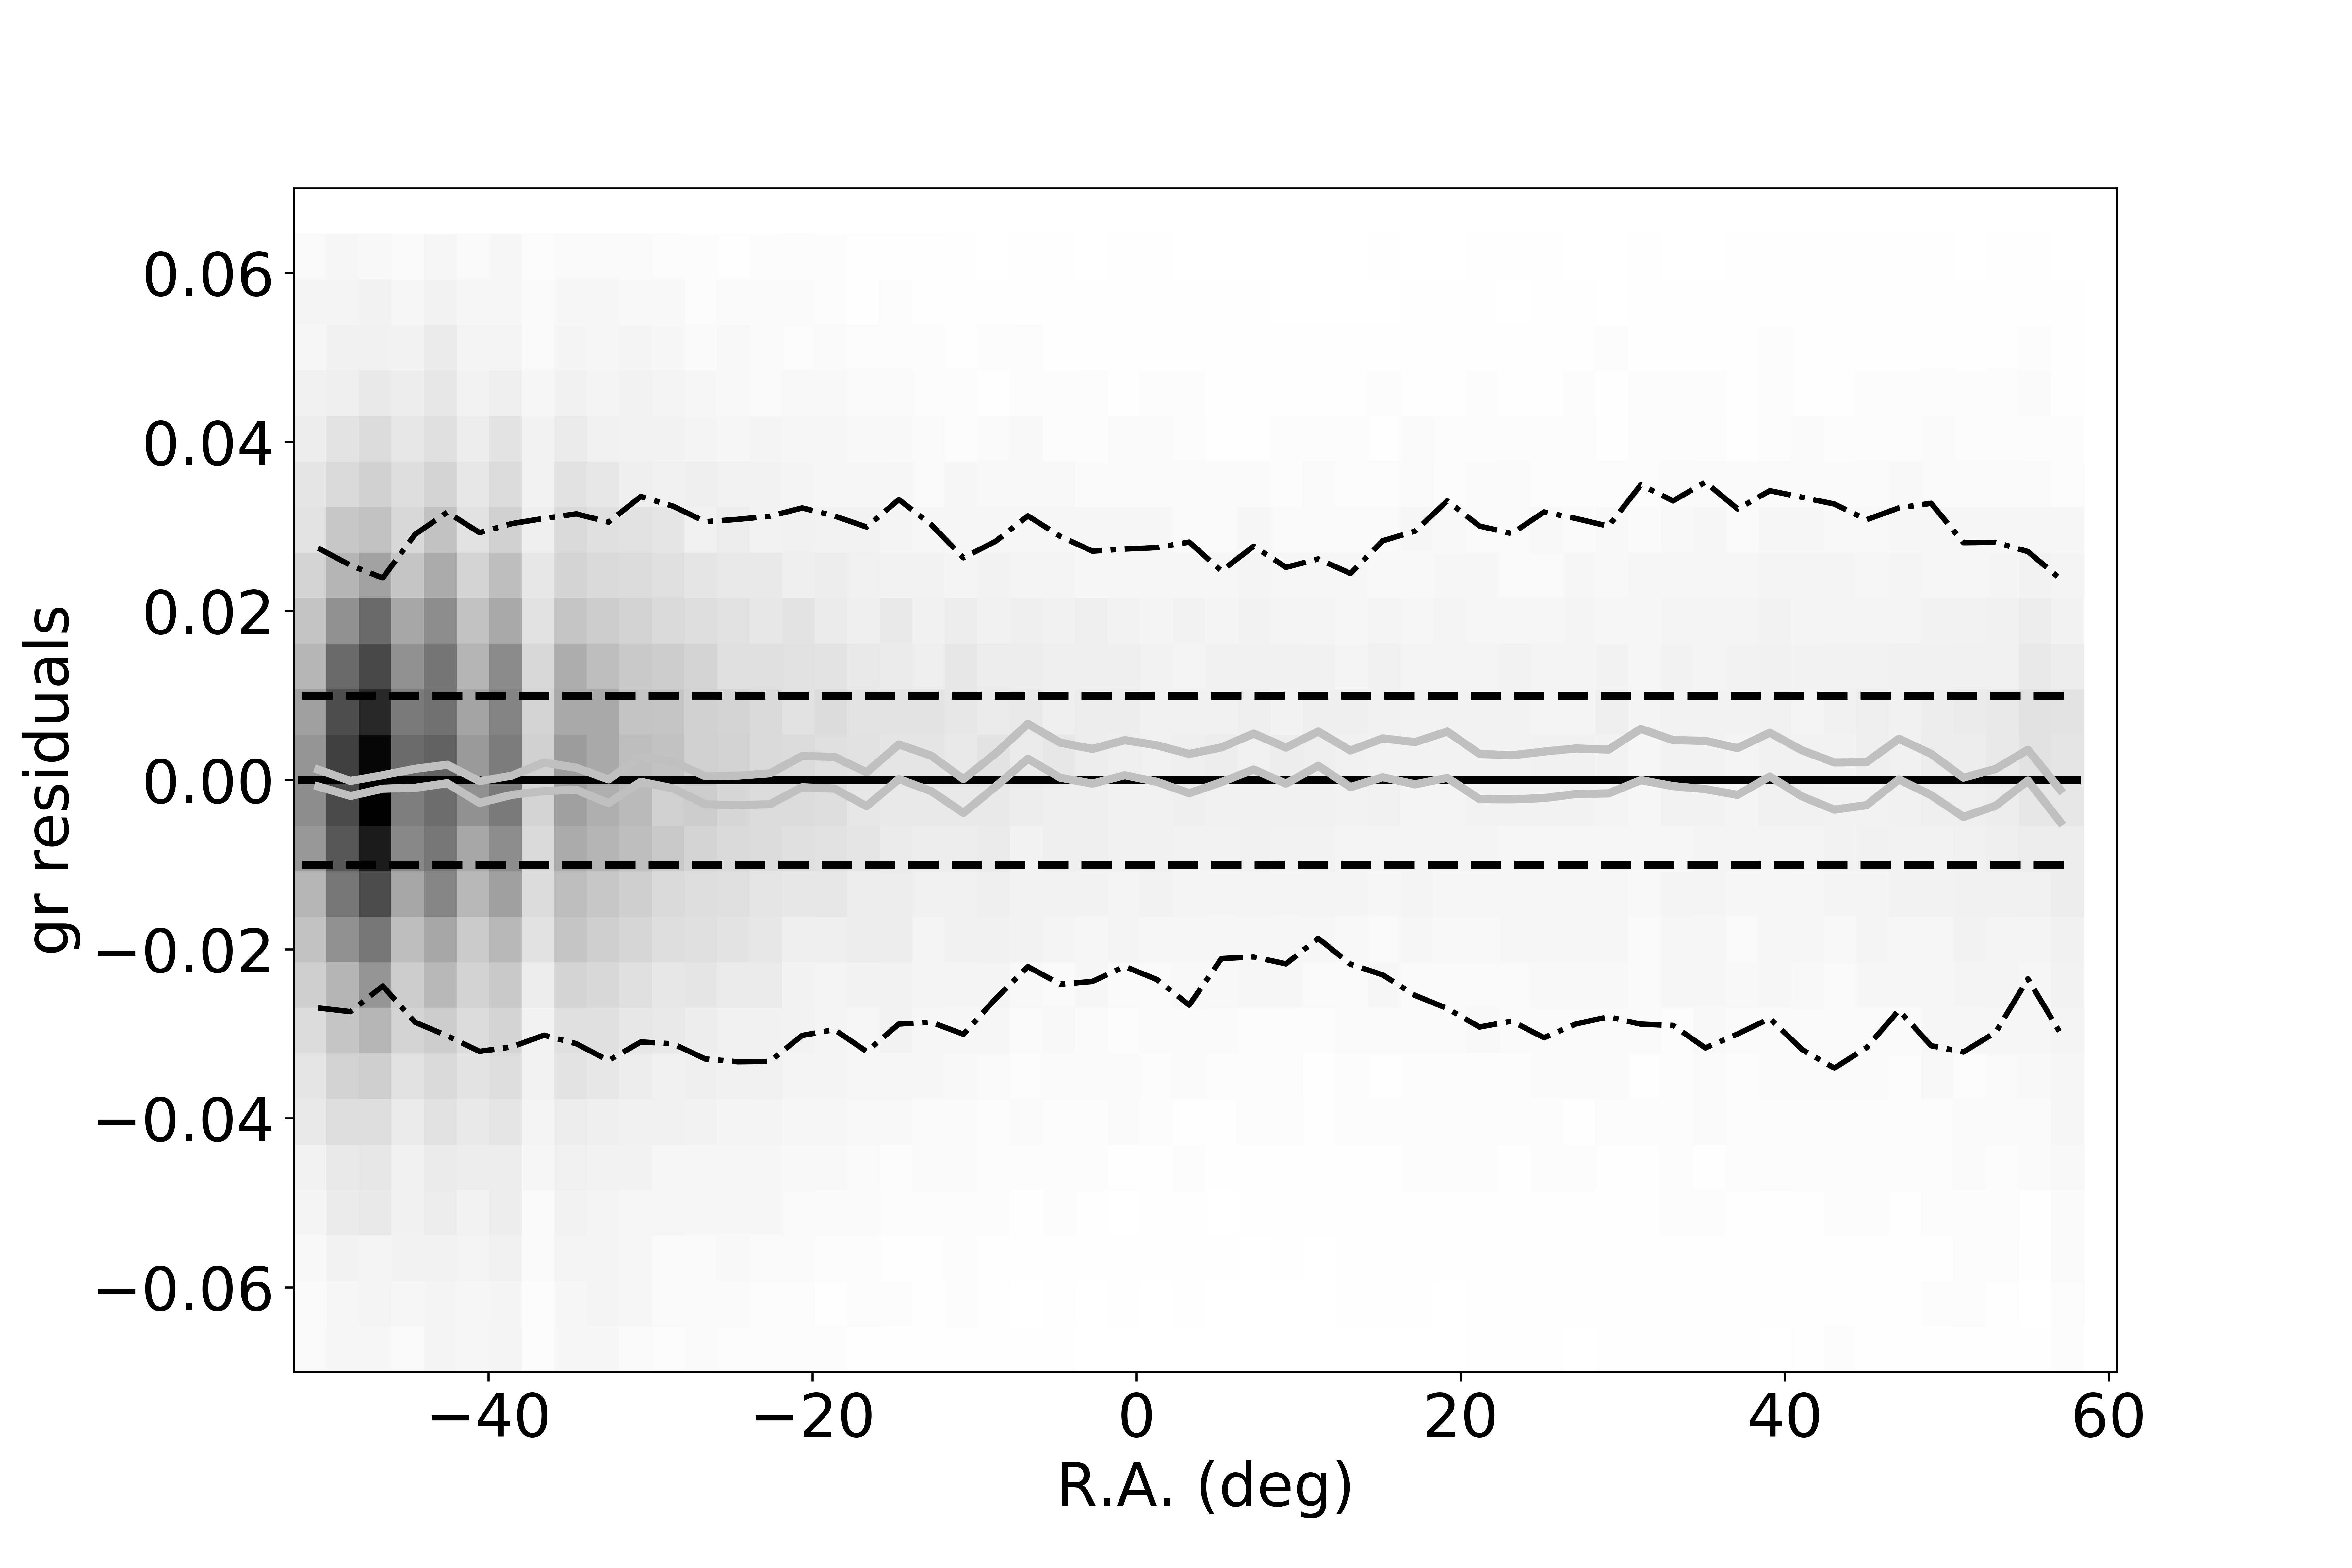
\includegraphics[width=7cm]{figures/colorResidGaiaColors_gr_RA_Hess.png} 
    \centering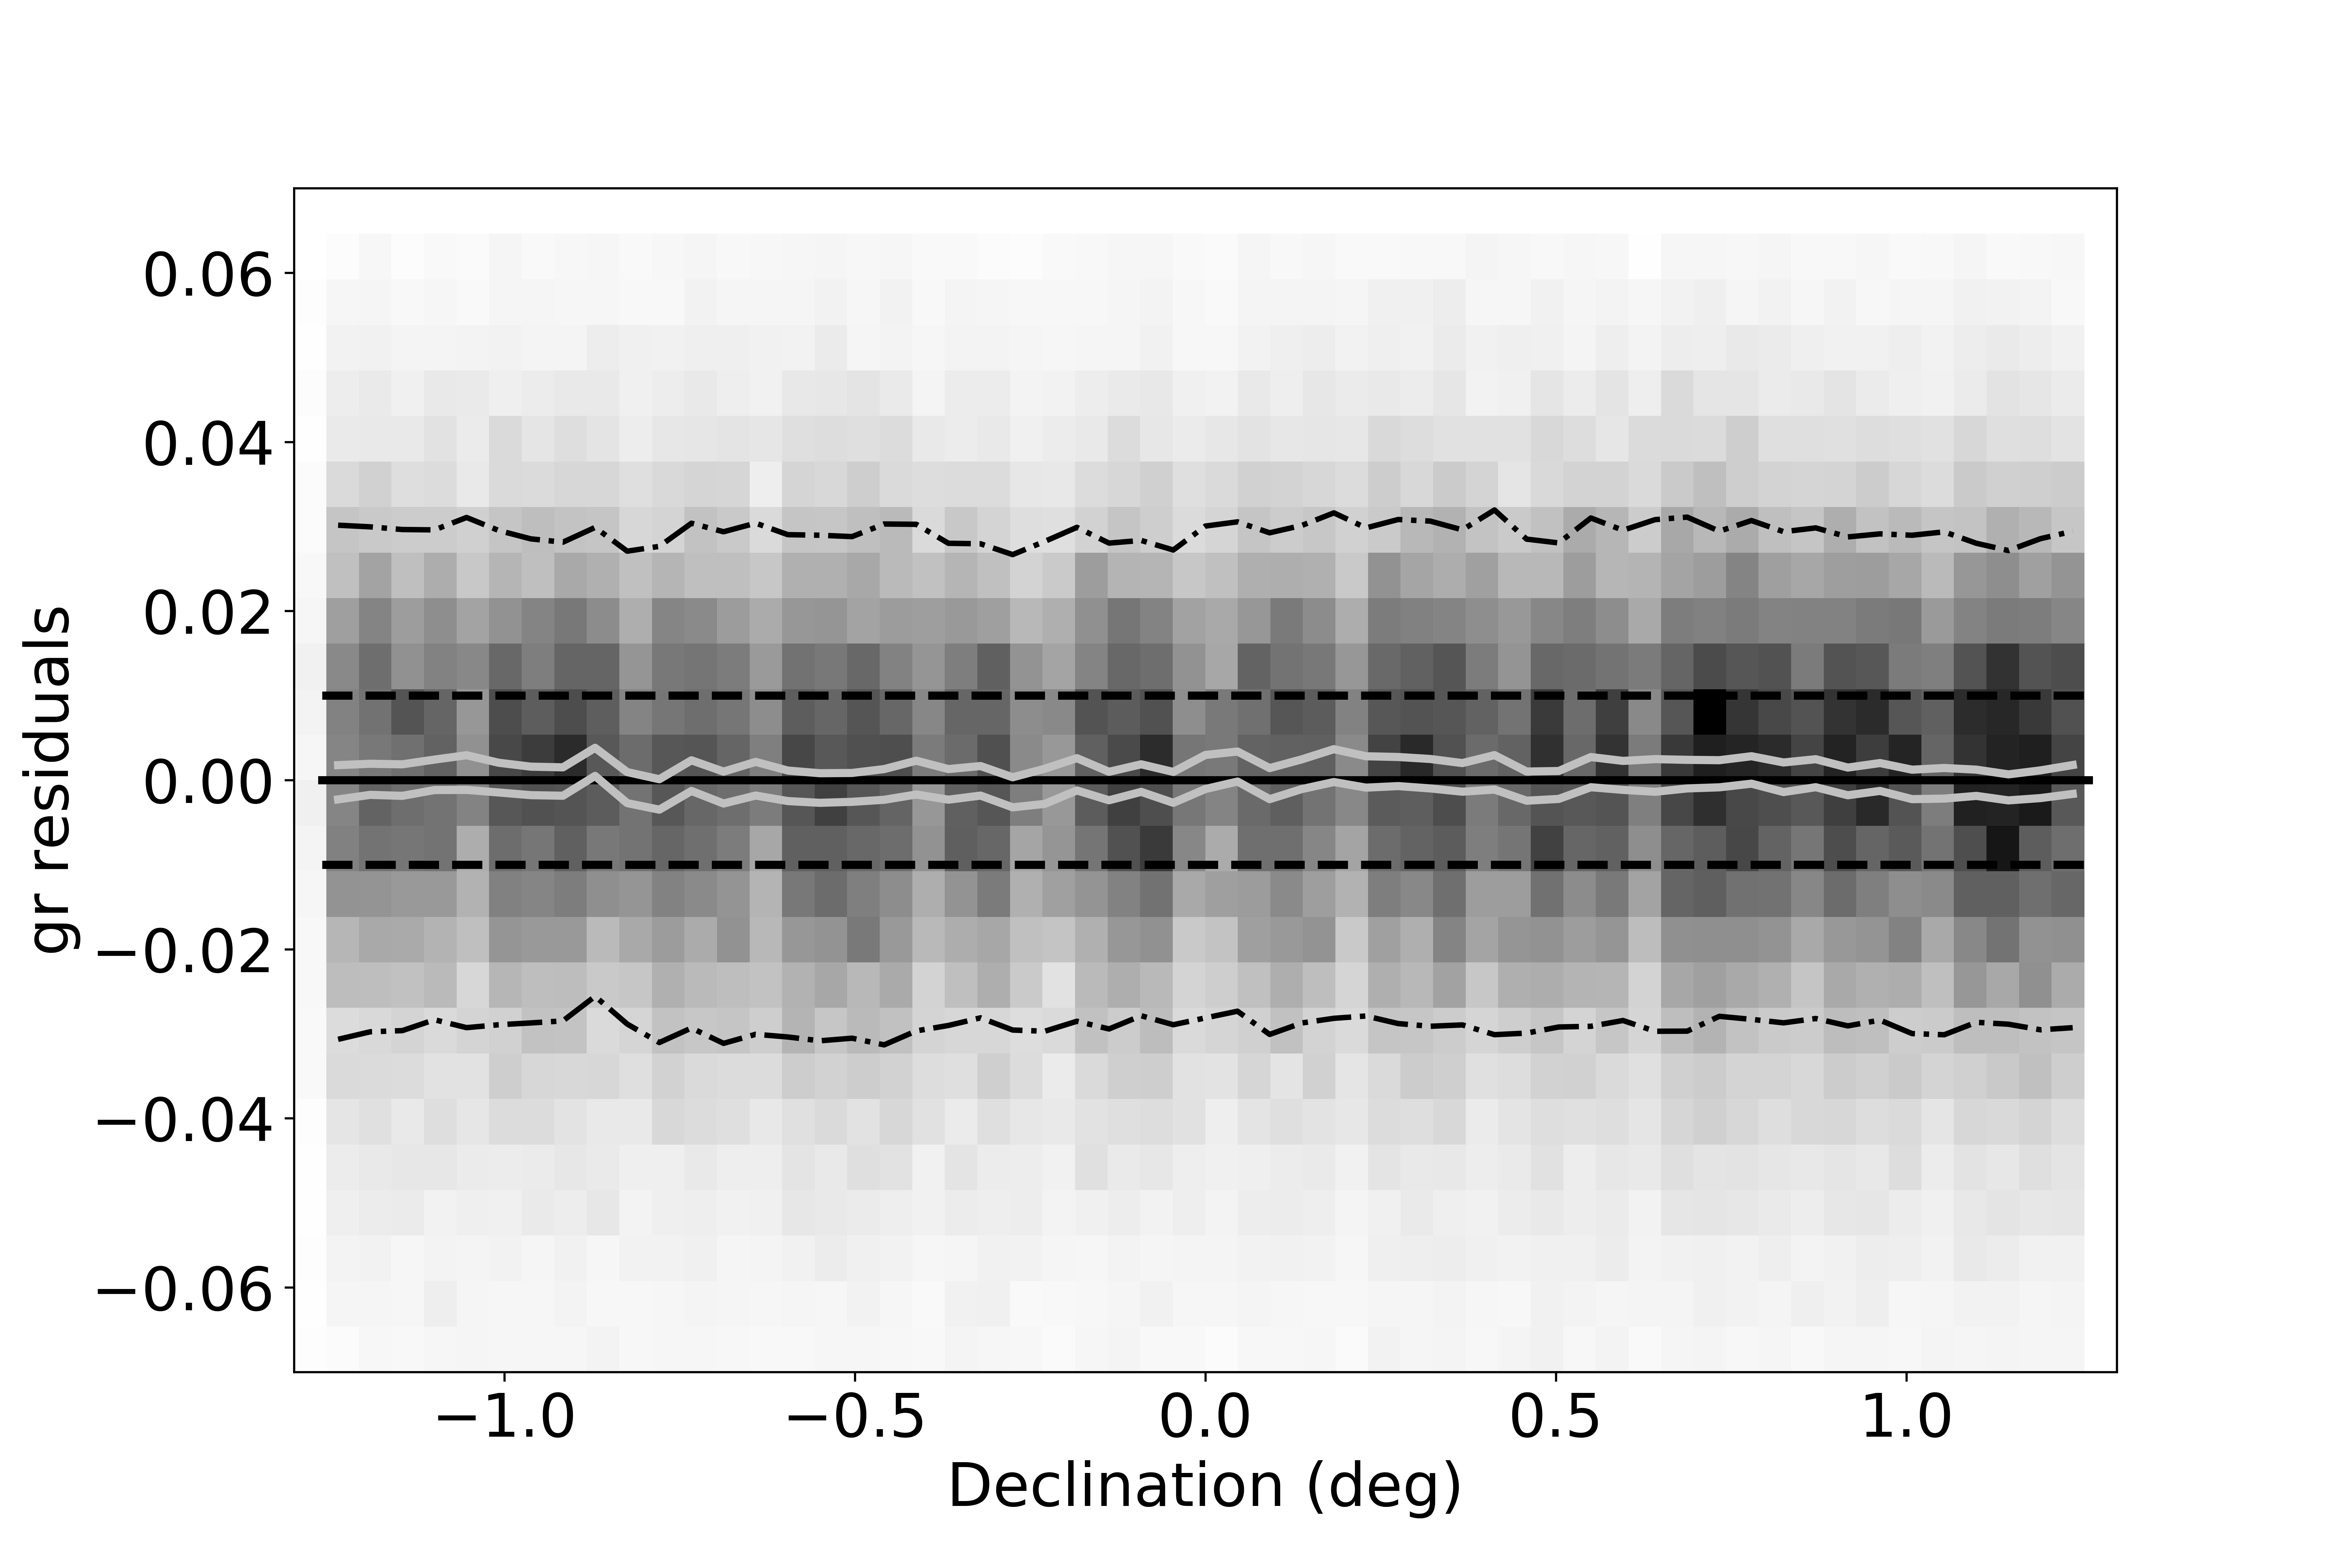
\includegraphics[width=7cm]{figures/colorResidGaiaColors_gr_Dec_Hess.png} 
\caption{Left: analogous to Figure~\ref{fig:graycorrRA}, except that here residuals between
the SDSS $g-r$ color from the v3.4 catalog and a synthetic $g-r$ color generated using 
Gaia's $BP-RP$ color are shown. The binned median scatter is 1.6 millimag. Right: the 
$g-r$ residuals are shown as a function of Declination. The binned median scatter is 
0.8 millimag.}
\label{fig:grVSgaiaRADec}
\end{figure}
 

\subsection{Comparison of the SDSS v2.6 and v3.4 catalogs \label{sec:v26v34}} 
 
The v2.6 (``old'') SDSS Standard Star Catalog has been extensively used 
\citep[e.g.,][]{2008AJ....135..338F},
and here we briefly analyze differences between the v3.4 (``new'') and v2.6 magnitudes
to inform the future users about catalog consistency. 
In our analysis, we first compare v2.6 and v3.4 magnitudes of individual stars and 
bin the differences by R.A., Declination and magnitude. 

On average, both catalog versions are on the same magnitude scale (the median $ugriz$ 
magnitude differences for all stars are zero by construction). There are no systematic offsets 
when binned by magnitude, as illustrated in Figure~\ref{fig:v26v34drr}. The most obvious 
differences appear when magnitude differences are binned by Declination. An example is 
shown in Figure~\ref{fig:v26v34drDec}, where the periodicity of residuals corresponds to the 
field-of-view size for the SDSS Photometric Telescope \citep{2006AN....327..821T}. 
The standard deviation for median values per bin is 6.8 millimag, with extreme values about 
0.01 mag. It is likely that systematic errors in the calibration star network photometry 
were propagated through ``flat-field corrections'' discussed by \pO\ to the v2.6 catalog.
We note that these errors, now found thanks to Gaia catalogs, are well within the claimed
photemetric accuracy by both \pO\ and \cite{2002AJ....123.2121S}. The standard deviation 
for median values per bin for all bands and both coordinates is listed in Table~\ref{tab:oldnewRMS}. 


\begin{deluxetable}{l|c|c}[ht!]
\tablecaption{The robust standard deviation for magnitude differences between the v2.6 (old)
and v3.4 (new) catalogs. \label{tab:oldnewRMS}}
\tablehead{
\colhead{Band} & \colhead{rms for R.A.} & \colhead{rms for Dec}
}
\startdata
       $u$        &        2.3$^a$    &    25.5      \\
       $g$        &        4.5    &      9.4      \\  
       $r$         &        2.0    &      7.0      \\  
       $i$         &        5.3    &      6.5      \\ 
       $z$        &        8.9    &      8.4      \\ 
\enddata
\tablenotetext{a}{For the $u$ band, the scatter in R.A. direction is due to more observations
in v3.4 than in v2.6, rather than zeropoint correction.} 
\end{deluxetable}
   


\begin{figure}[th!]
    \centering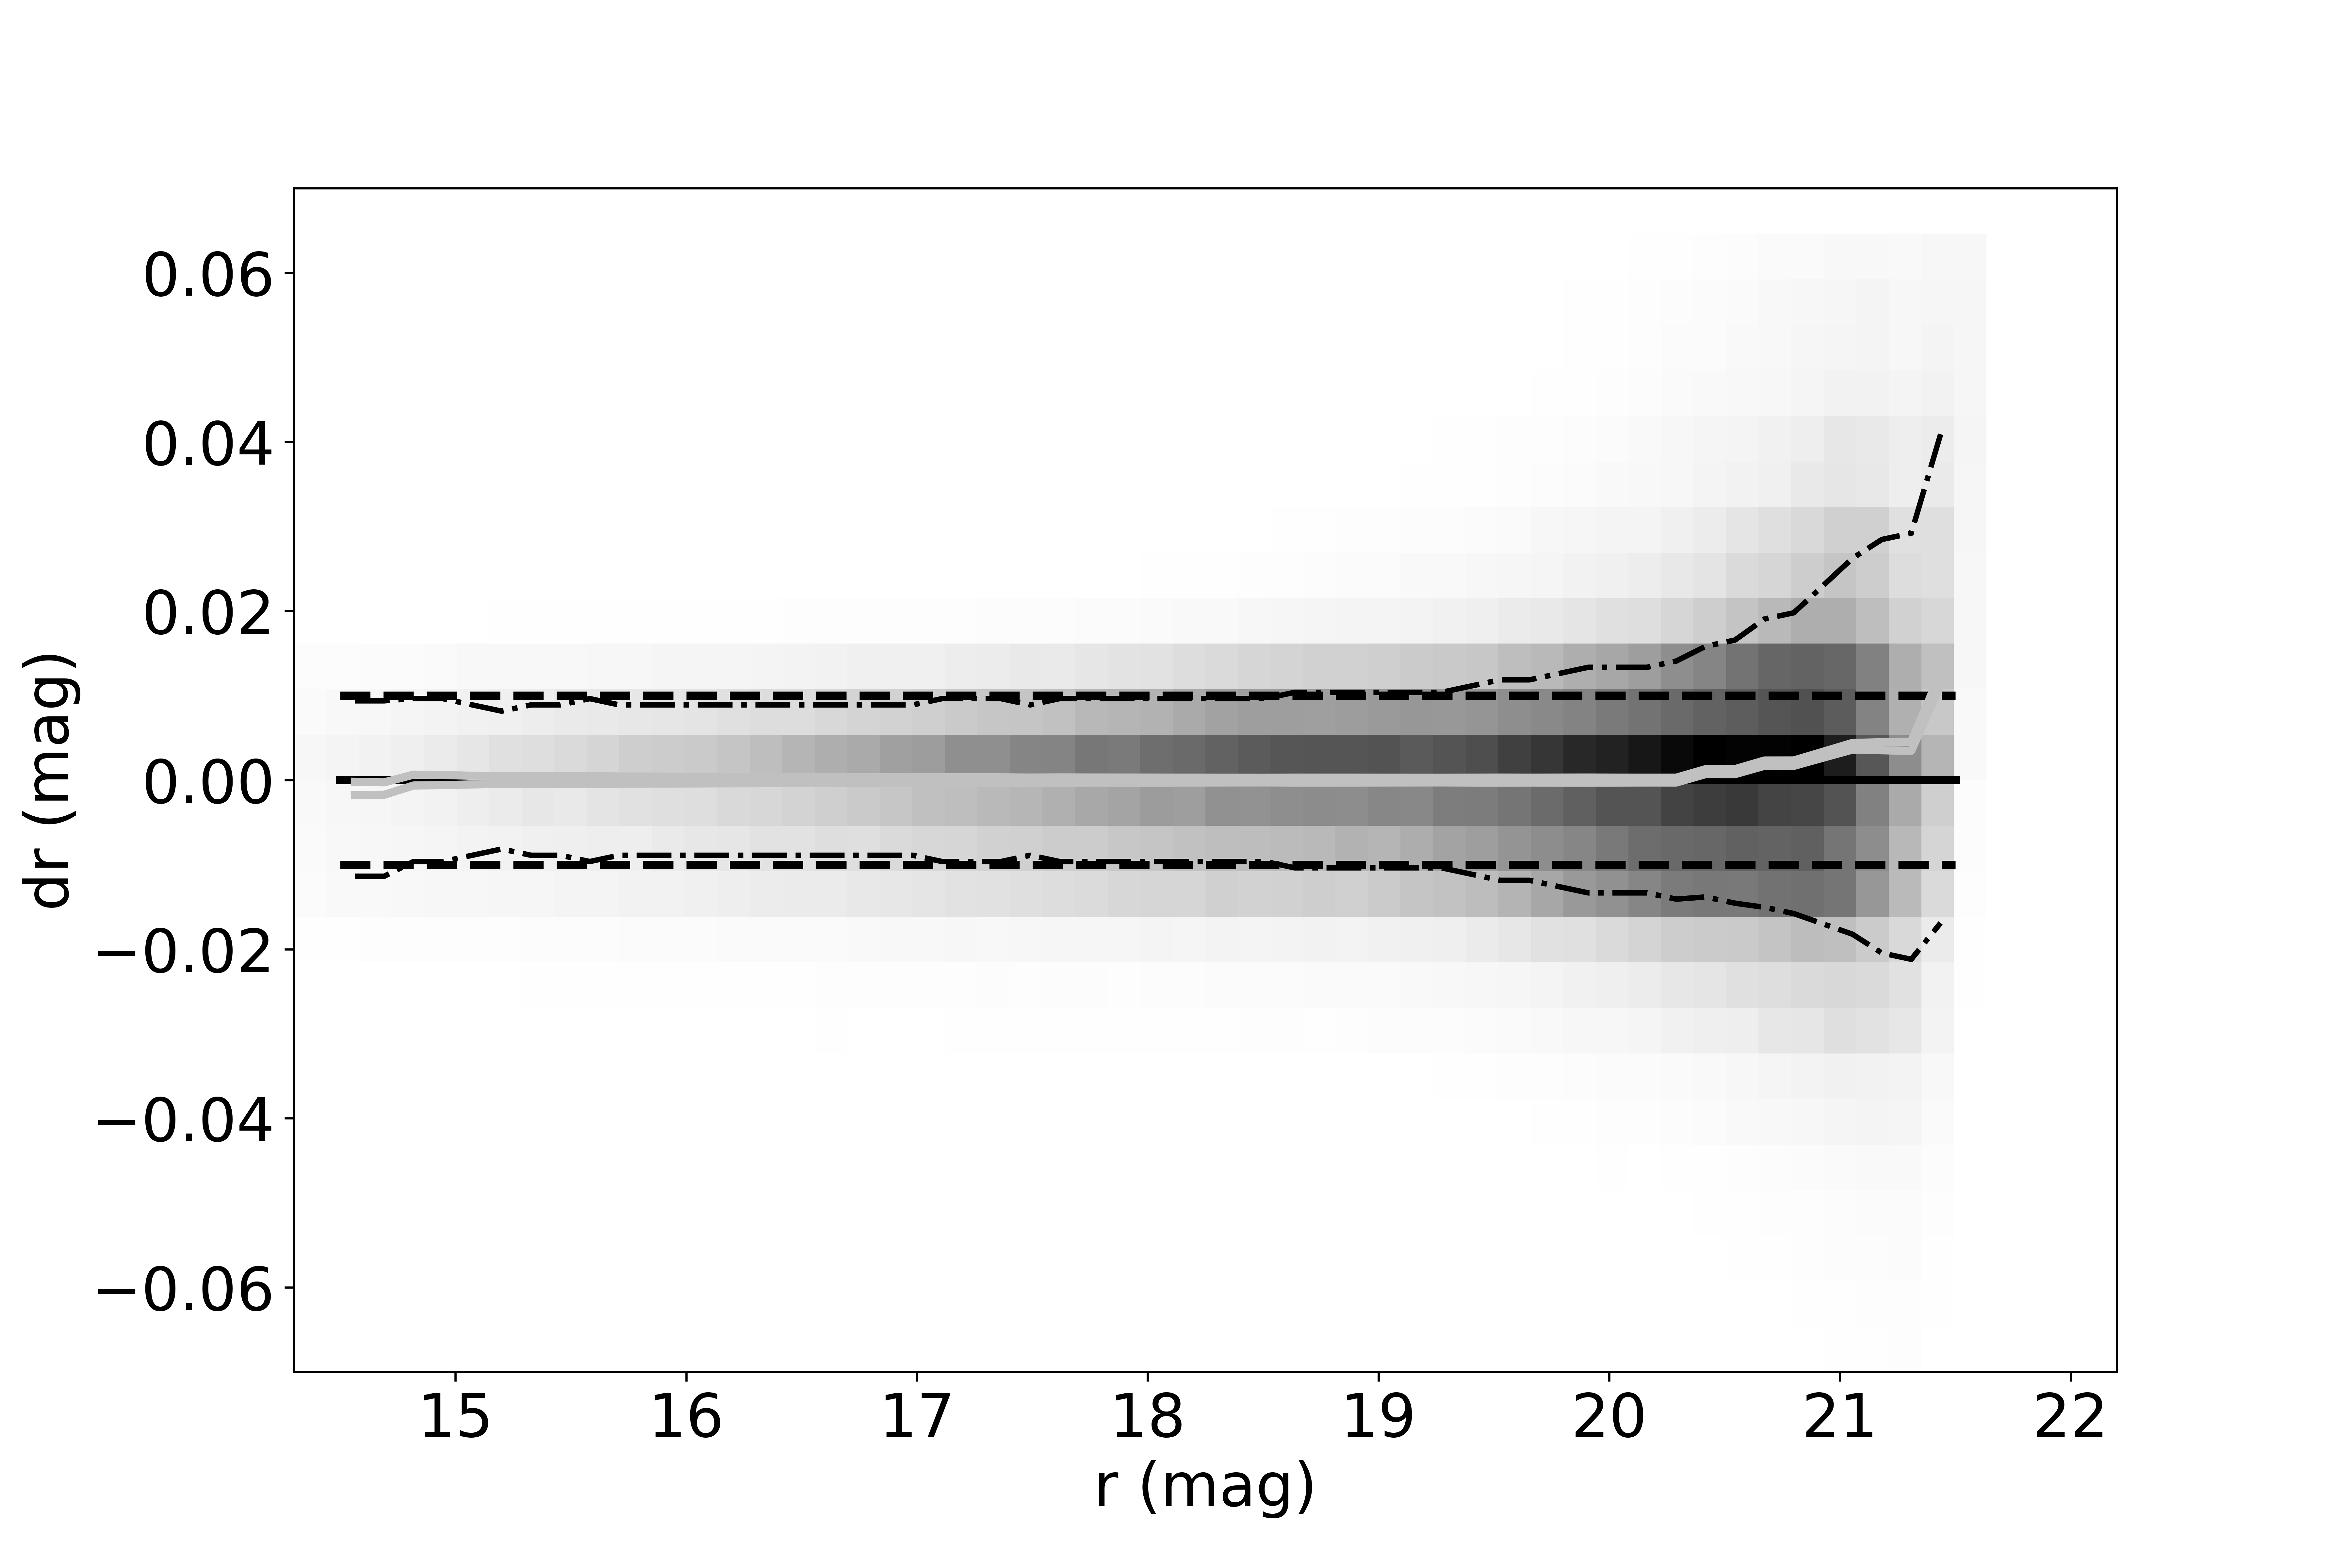
\includegraphics[width=9cm]{figures/testV26vsV33_r_dr_r_mag_Hess.png} 
\caption{Analogous to Figure~\ref{fig:v26v34drDec}, except that here the $r$ band
differences are shown as a function of the $r$ band magnitude. The scatted of median
values per bin is 1.9 millimag. The scatter of individual values is $\sim0.01$ mag
for $r<20$, and it is due to more data in the new catalog.} 
\label{fig:v26v34drr}
\end{figure}


\begin{figure}[th!]
    \centering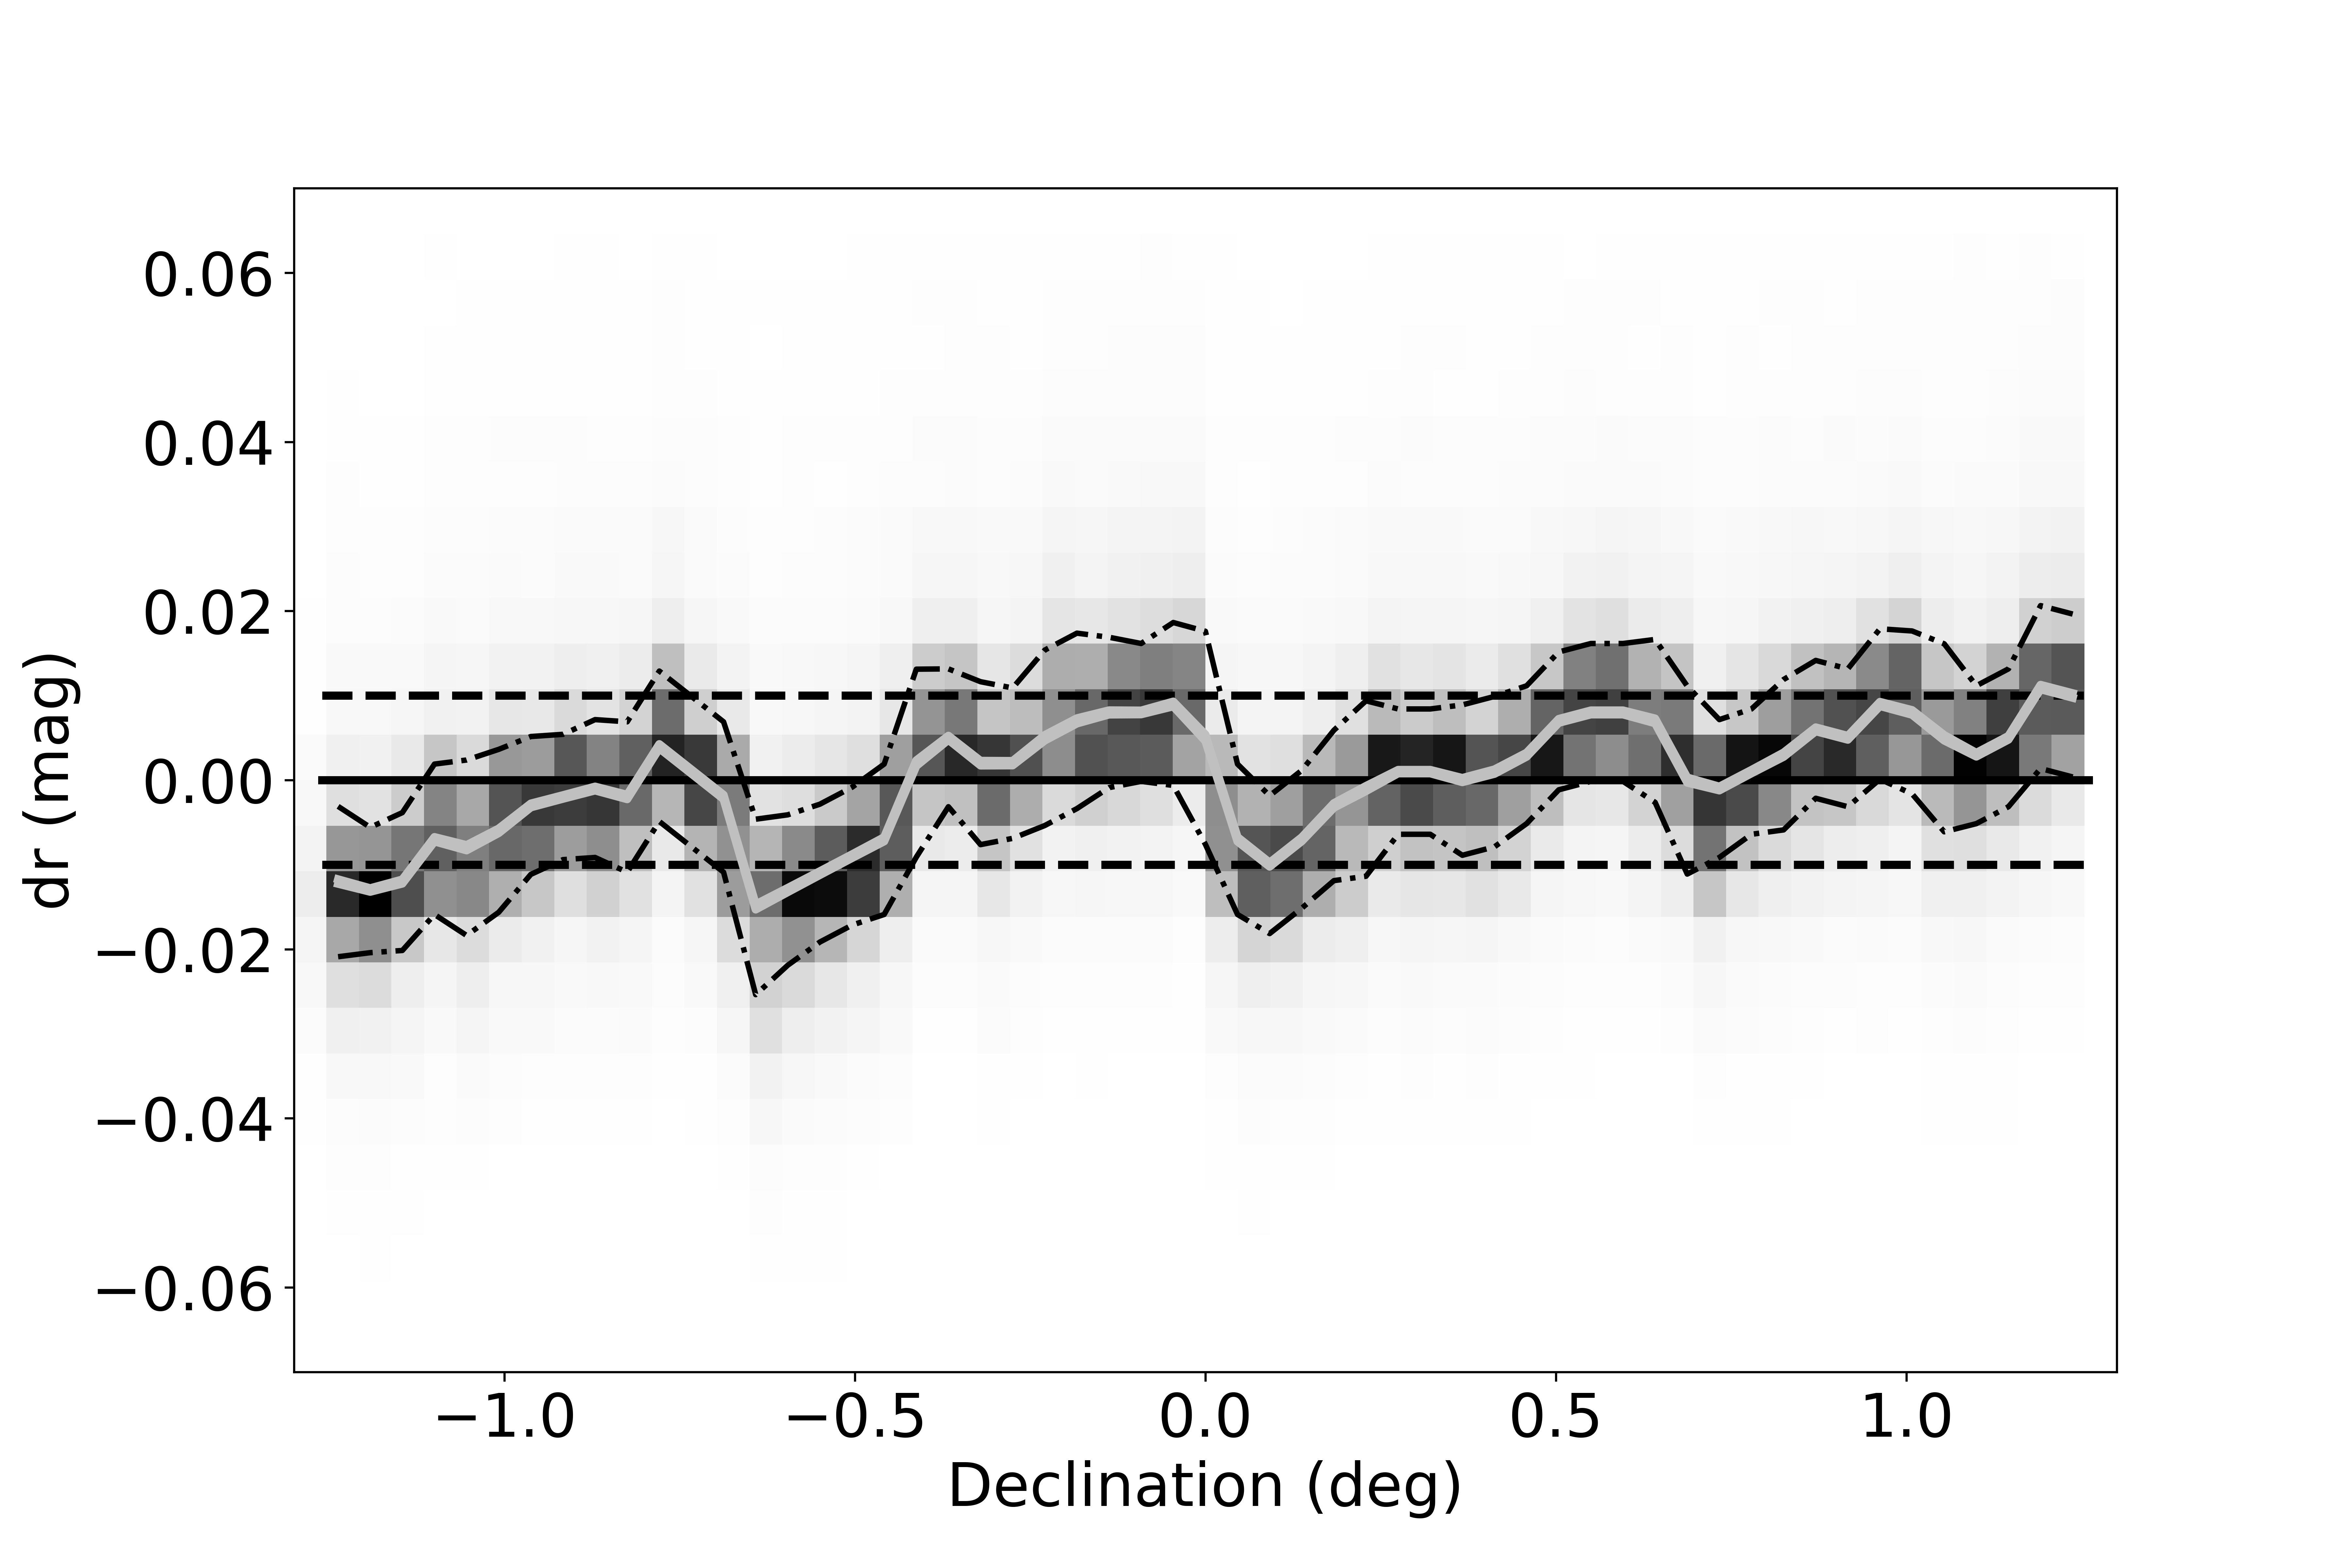
\includegraphics[width=9cm]{figures/testV26vsV33_r_dr_Dec_Hess.png} 
\caption{The differences between $r$ band magnitudes listed in the v2.6 and v3.4 
    SDSS Standard Star catalogs. The size of the four regions corresponds to the
field-of-view size of the SDSS Photometric Telescope. The standard 
deviation for median values per bin is 6.8 millimag, with extreme values about 0.01 mag. 
The scatter of binned medians in R.A. direction is much smaller -- 2.0 millimag. 
For statistics in other bands, please see Table~\ref{tab:oldnewRMS}.}
\label{fig:v26v34drDec}
\end{figure}
 


Given the quality of Gaia photometry, there should be no doubt that SDSS $ugriz$ photometry
reported in the new v.3.4 catalog is superior to the old v2.6 catalog. Nevertheless, we perform
additional tests, based on the position of the stellar locus in the $g-r$ vs. $u-g$, $r-i$ vs. $g-r$ 
and $i-z$ vs. $r-i$ color-color diagrams  \citep{2004AN....325..583I}. The tests are based
on the second principal color for the blue part of the stellar locus, whose median should 
not deviate from zero by construction. Figure~\ref{fig:comparew} compares the behavior
of the $w$ color for the old v2.6 and new v3.4 catalog and demonstrates that the $gri$
photometry is better calibrated in the latter. The behavior of the $s$ and $y$ colors for the 
new catalog is shown in Figure~\ref{fig:comparesy}. {\it Based on these tests, we find that 
the contribution of the zeropoint errors is $<5$ millimag to $gri$ photometry, and 
$<10$ millimag for the $u$ and $z$ bands.} 



\begin{figure}[th!]
    \centering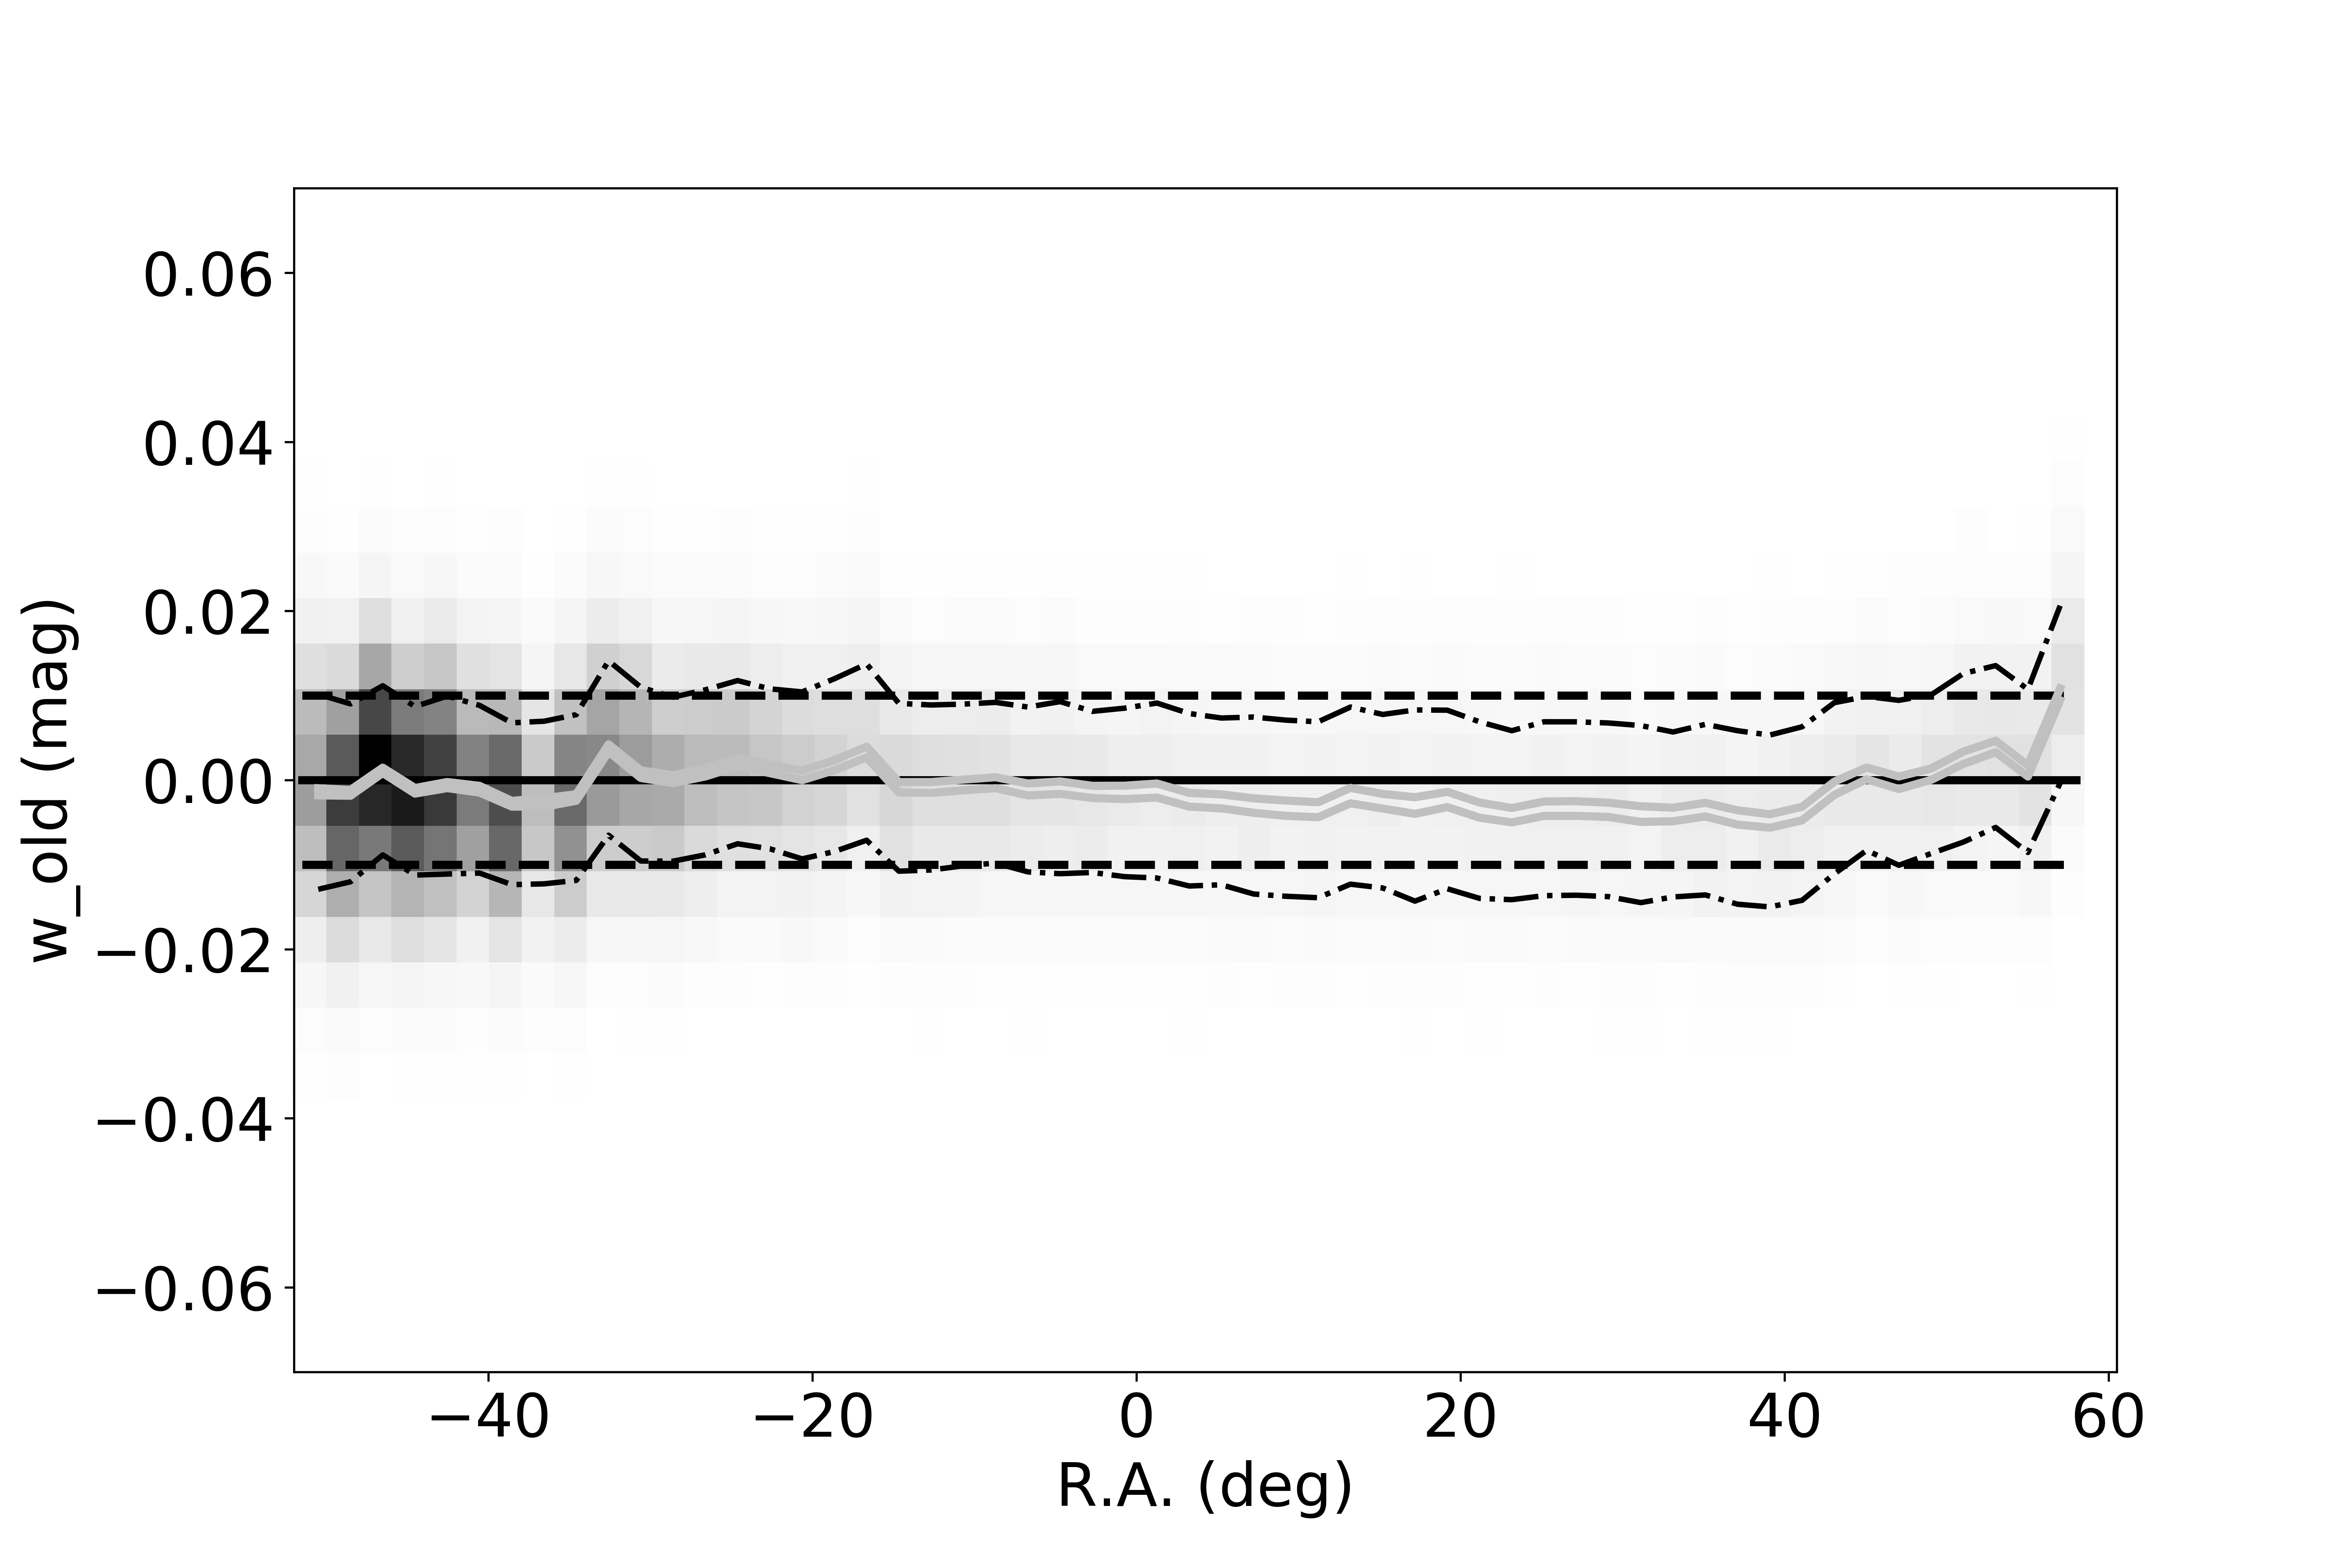
\includegraphics[width=7cm]{figures/testV26vsV33_r_w_old_RA_Hess.png}
    \centering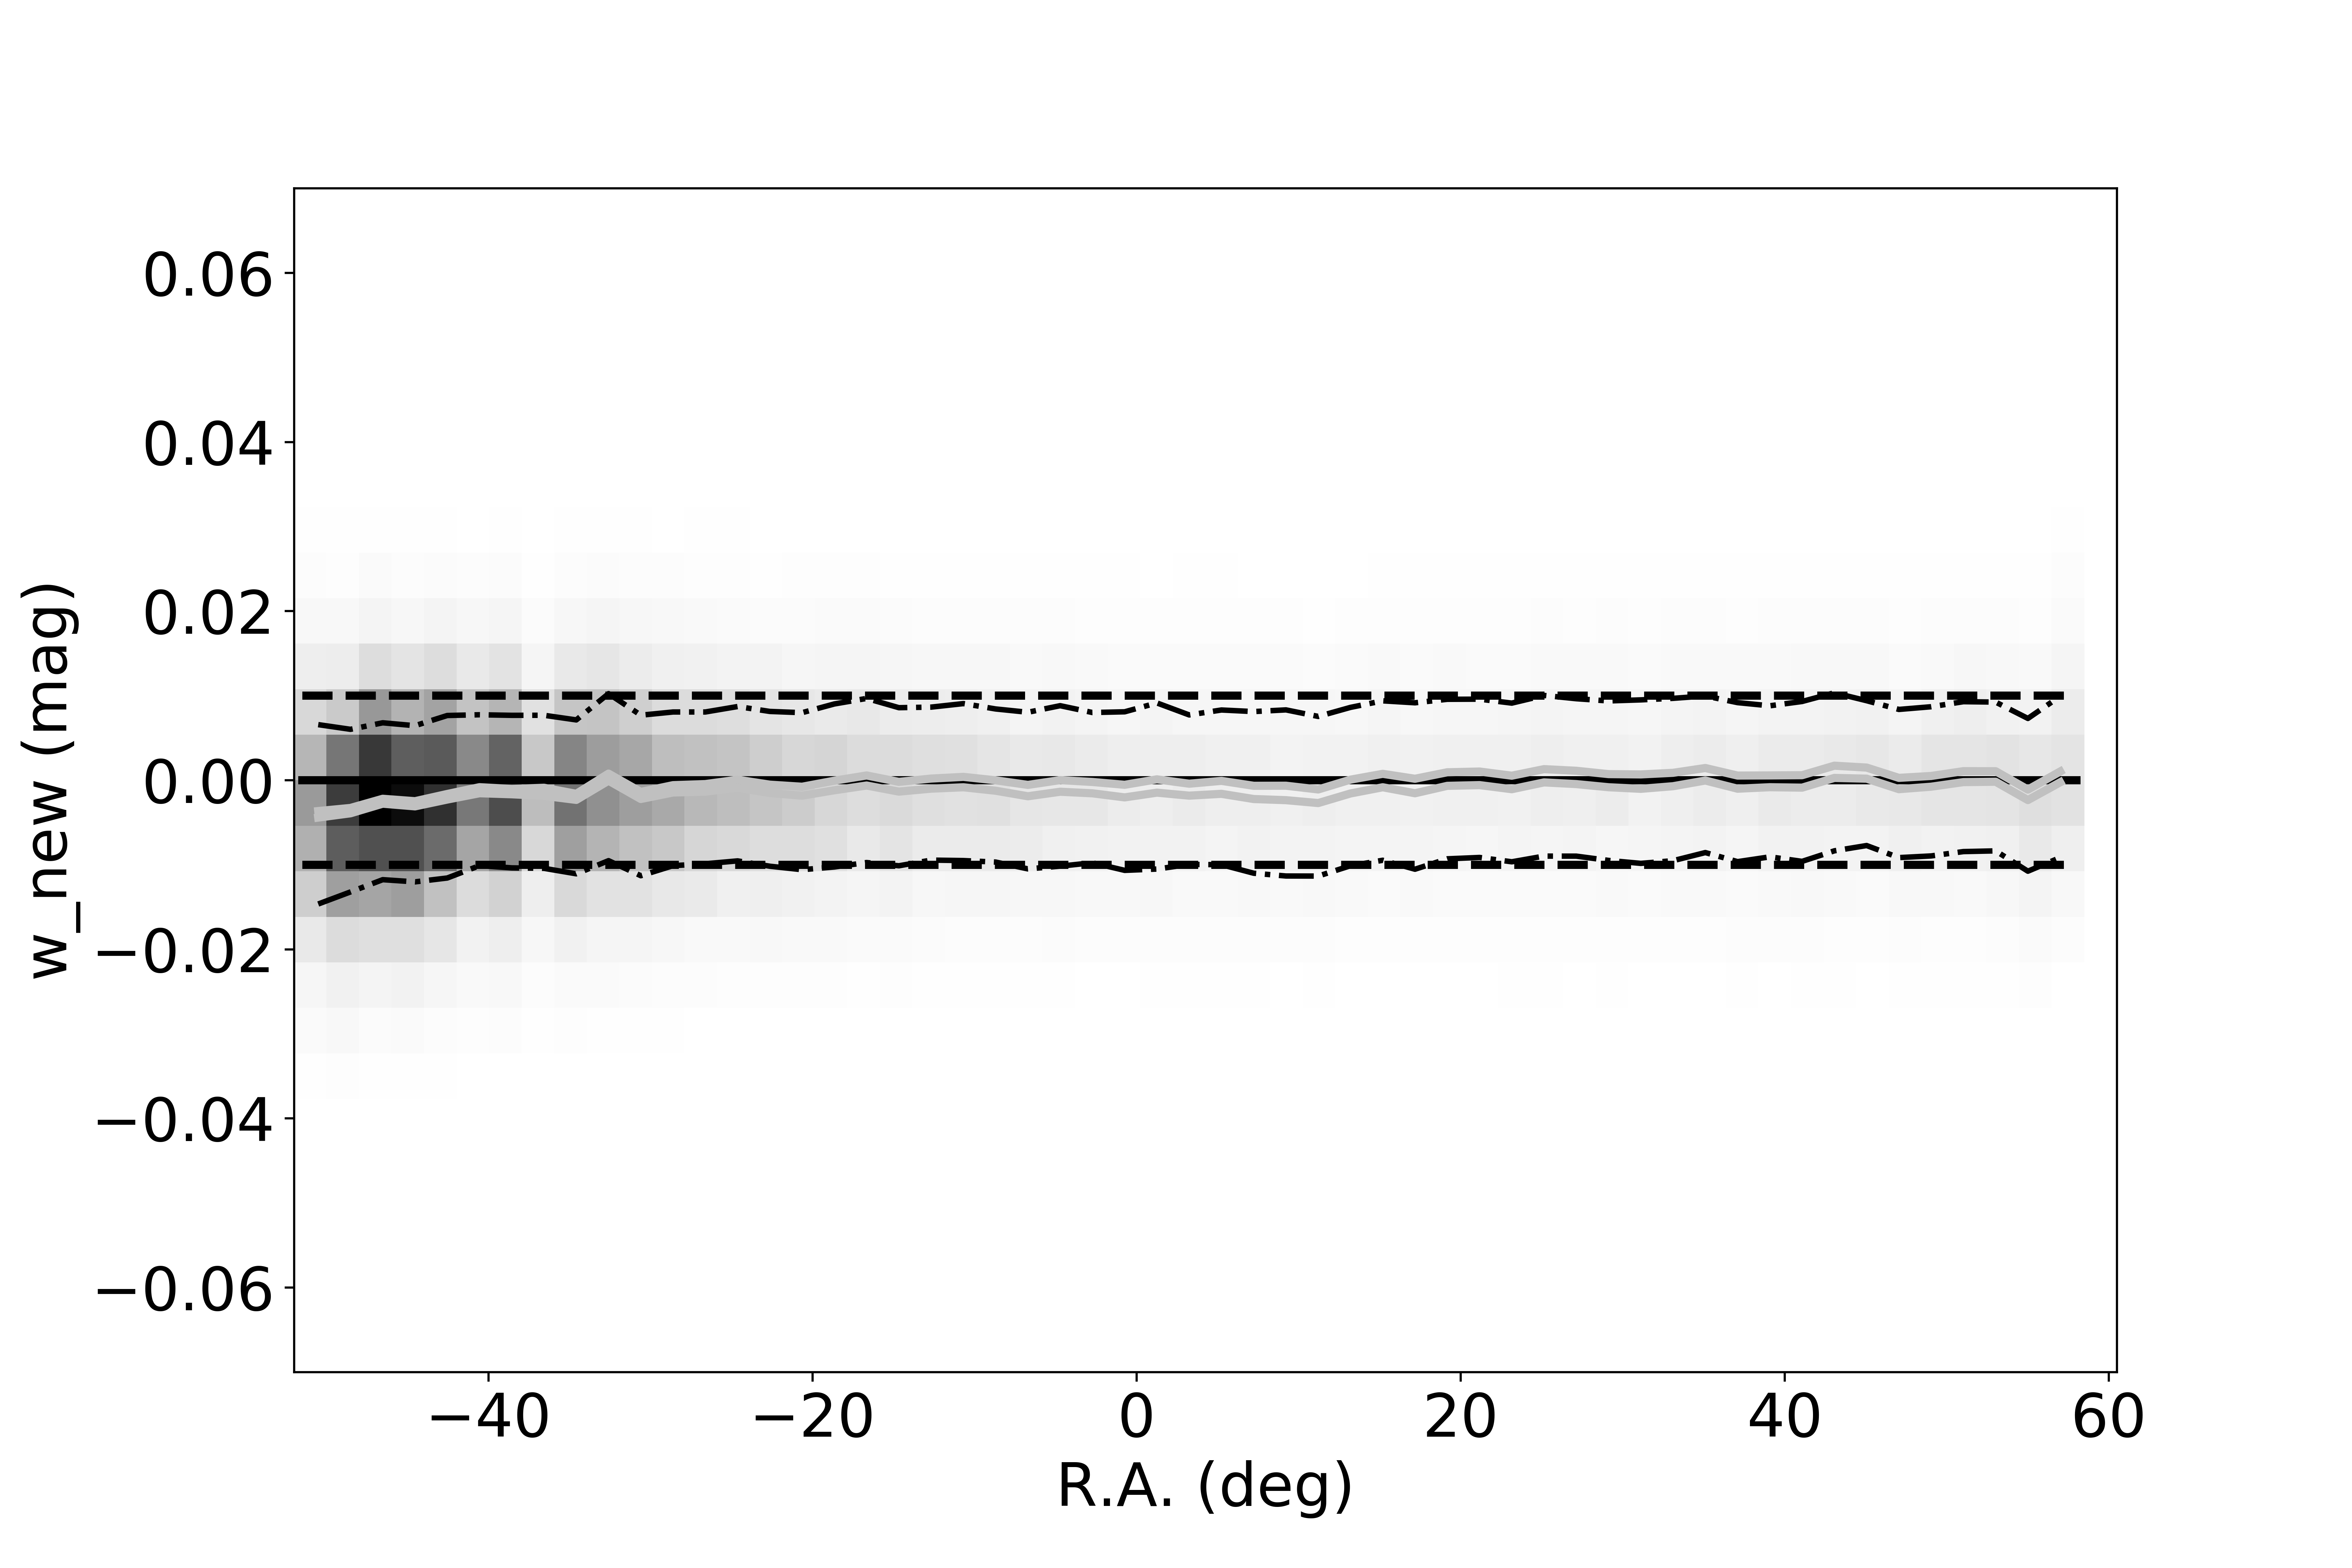
\includegraphics[width=7cm]{figures/testV26vsV33_r_w_new_RA_Hess.png}
    \centering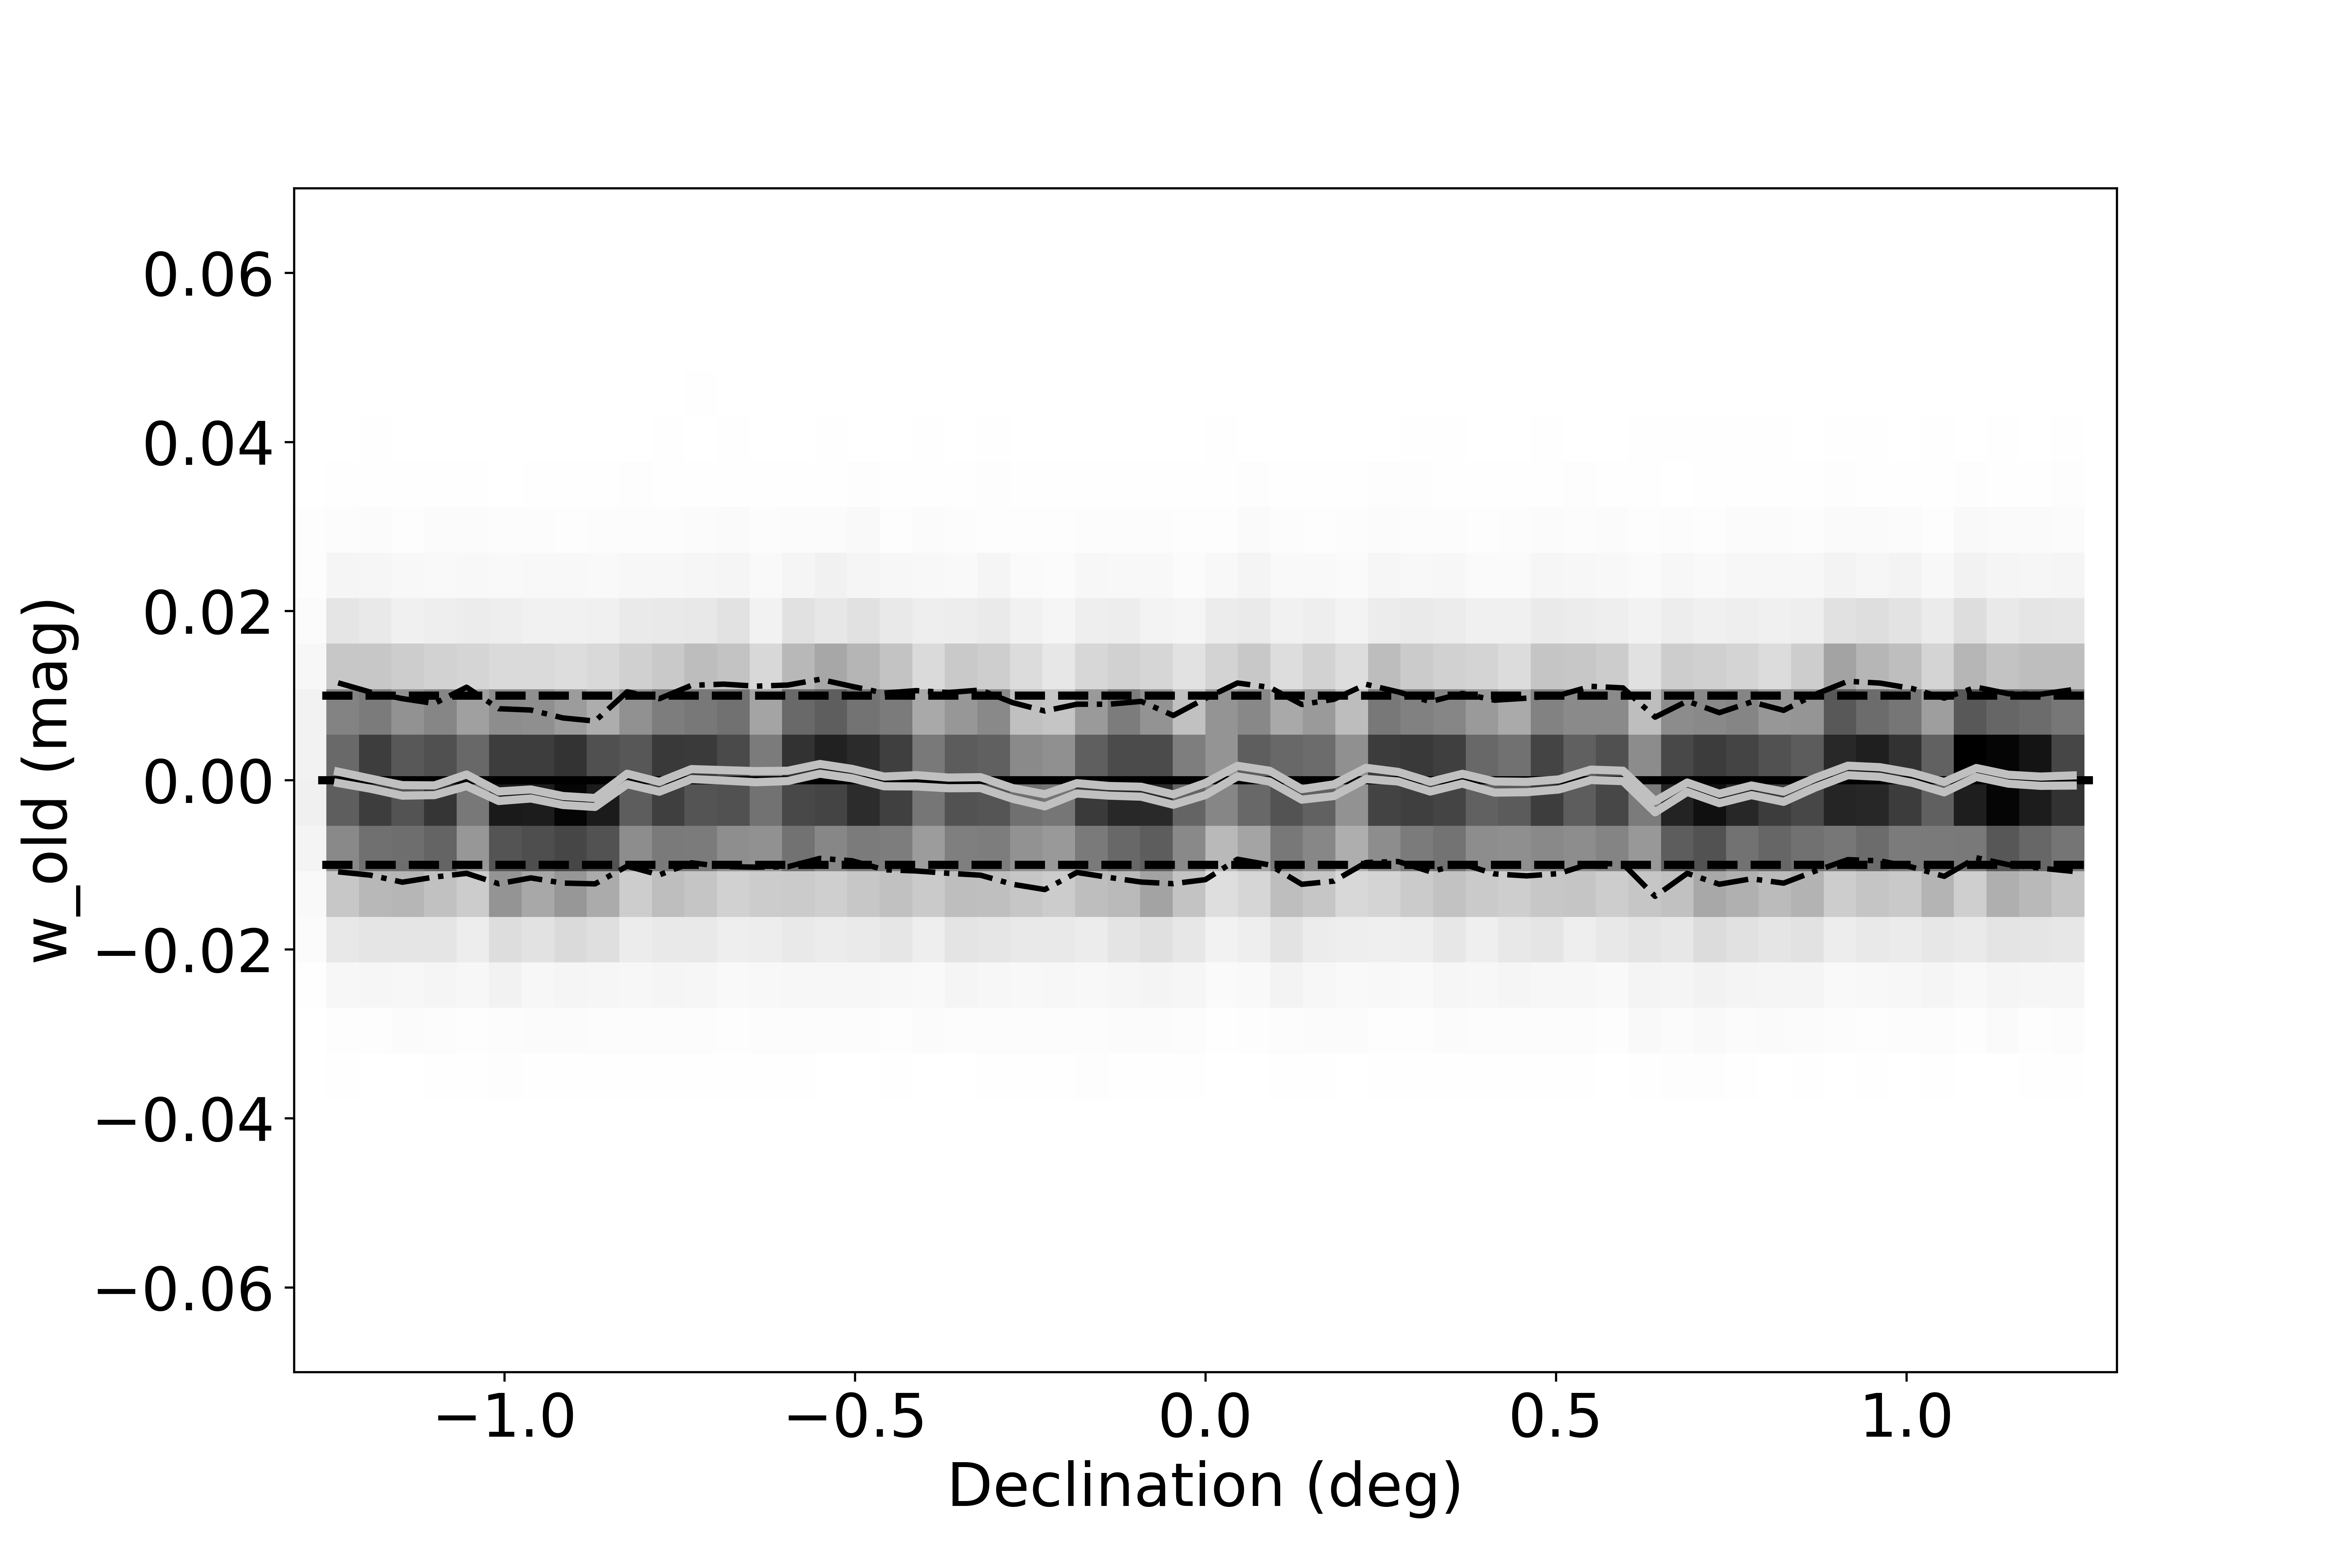
\includegraphics[width=7cm]{figures/testV26vsV33_r_w_old_Dec_Hess.png}
    \centering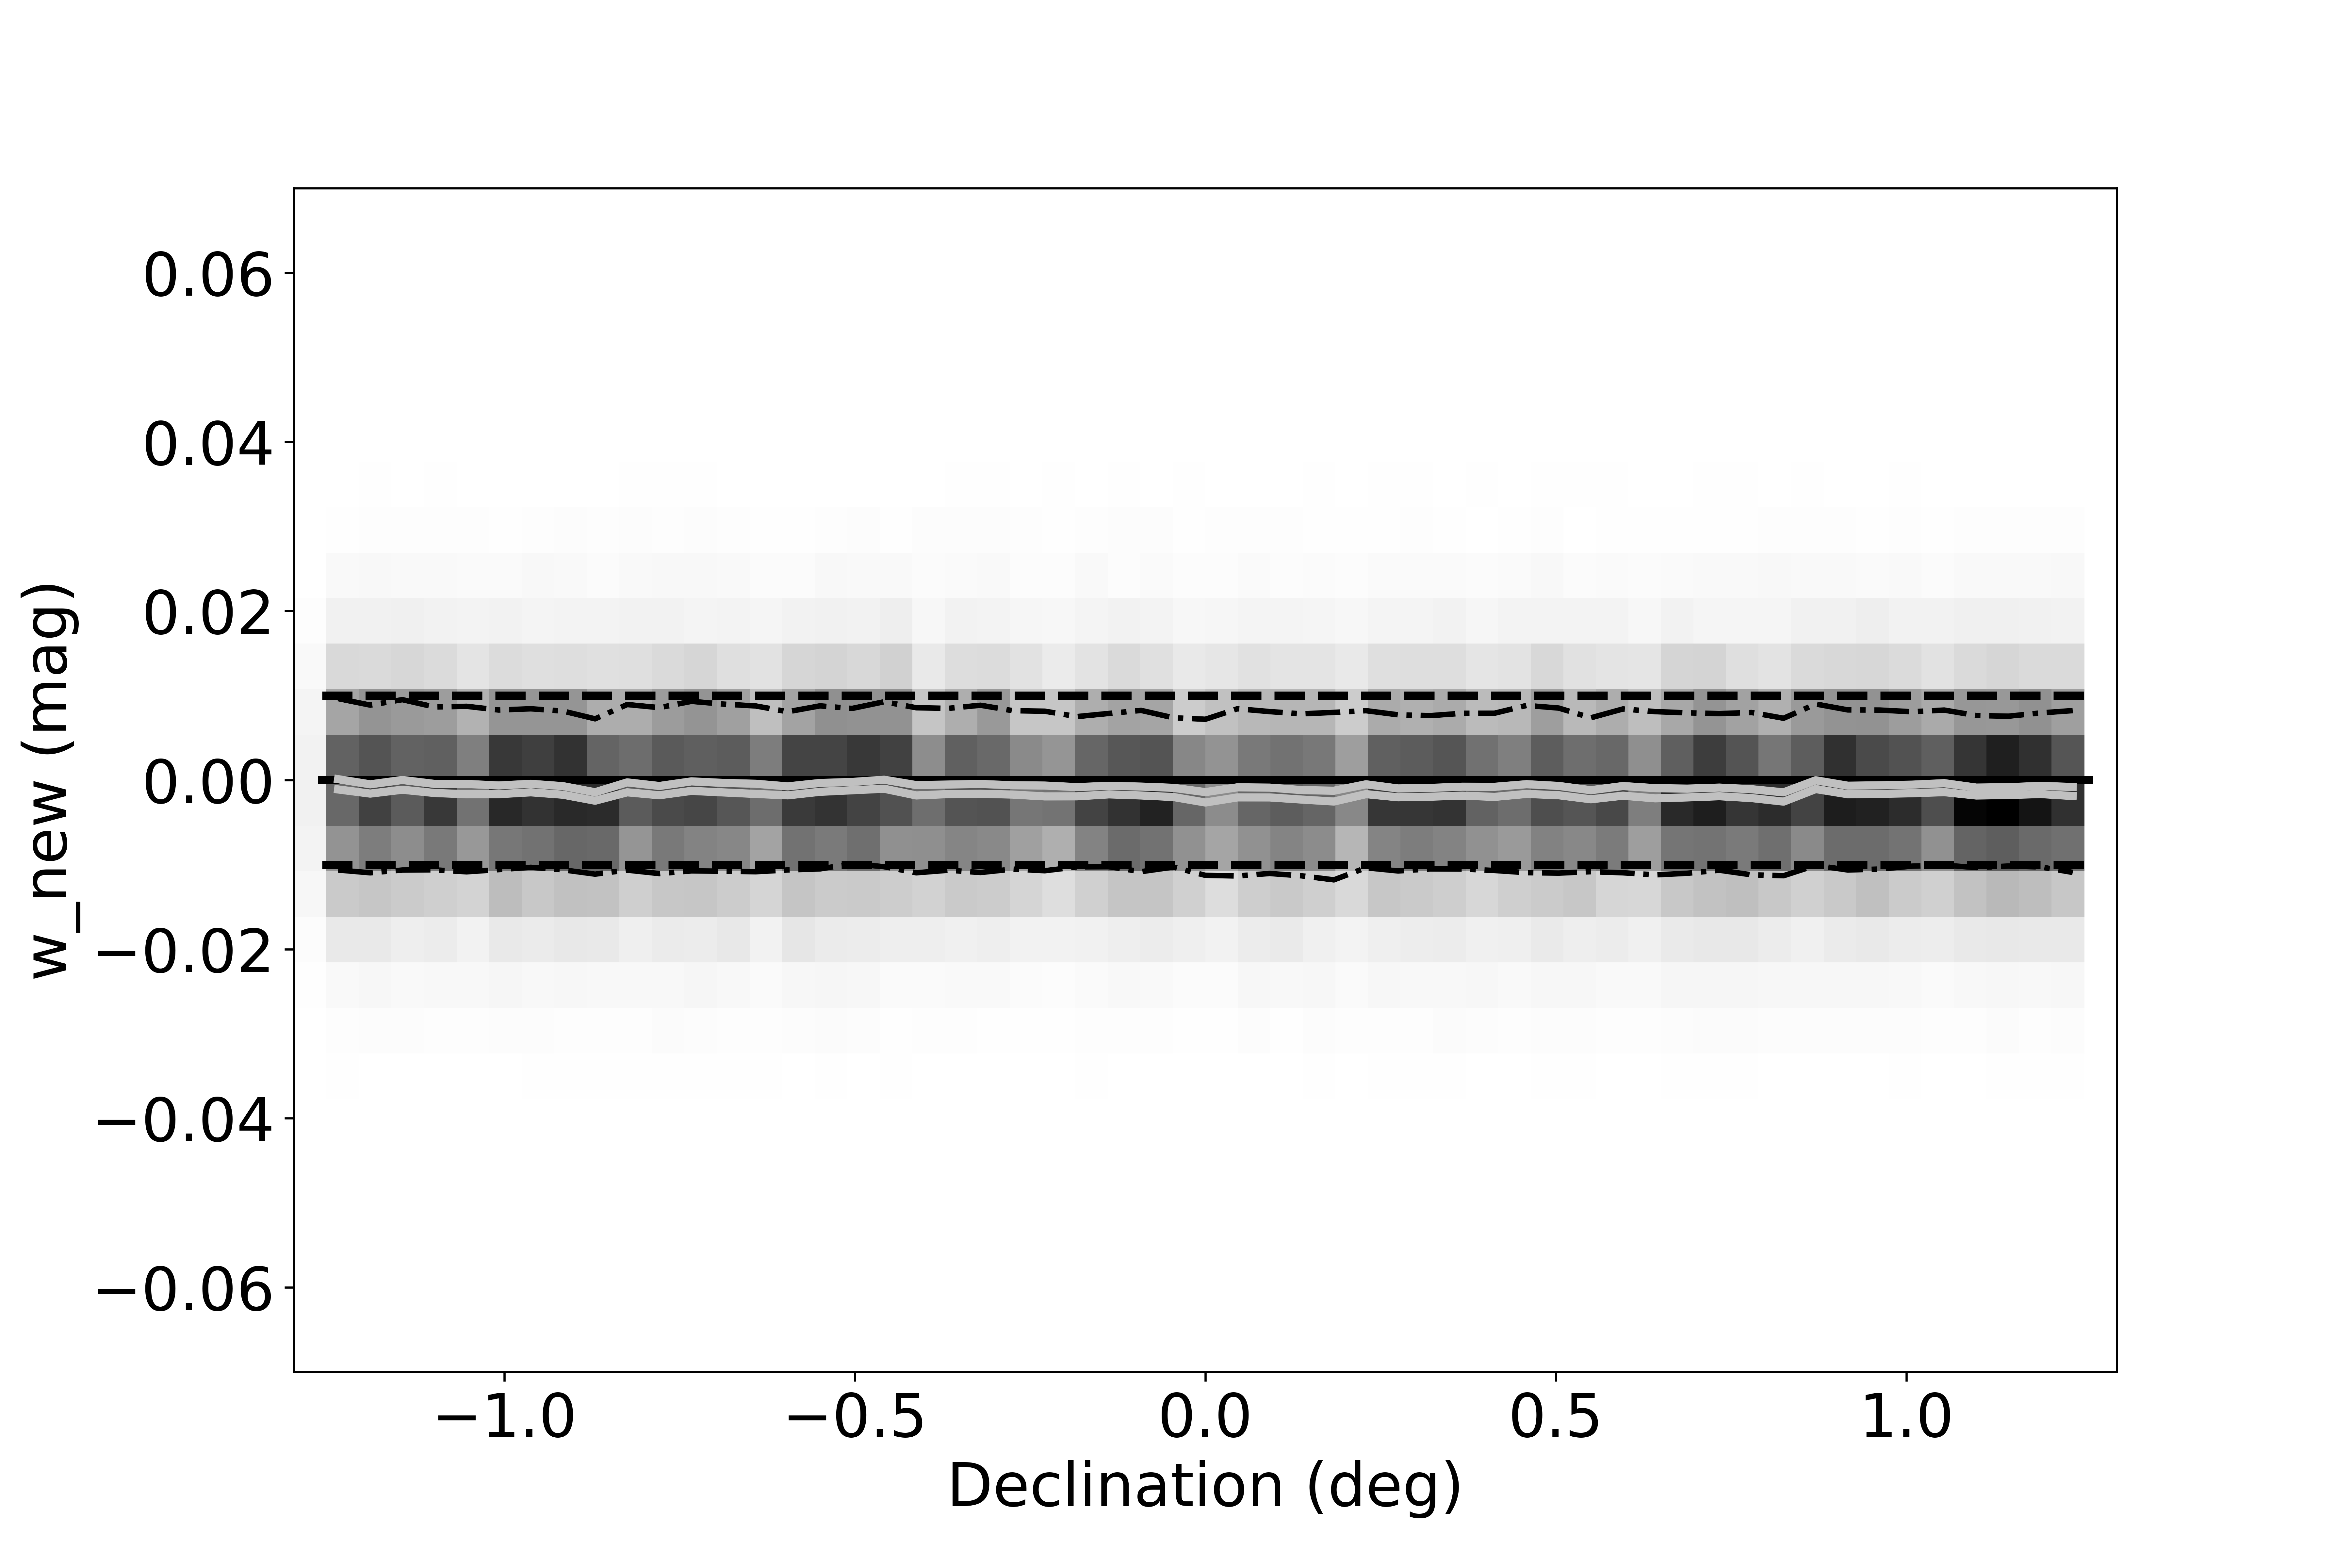
\includegraphics[width=7cm]{figures/testV26vsV33_r_w_new_Dec_Hess.png}
\caption{A comparison of the $w$ color, the second principal color in the SDSS
$r-i$ vs. $g-r$ color-color diagram, behavior for the v2.6 (left) and v3.4 (right)
catalogs. The standard deviation of the median $w$ values binned by R.A. and Dec
is 2.6 millimag and 1.1 millimag for v2.6 and 1.0 millimag and 0.3 millimag for v3.4,
respectively.}
\label{fig:comparew} 
\end{figure}
 

\begin{figure}[th!]
    \centering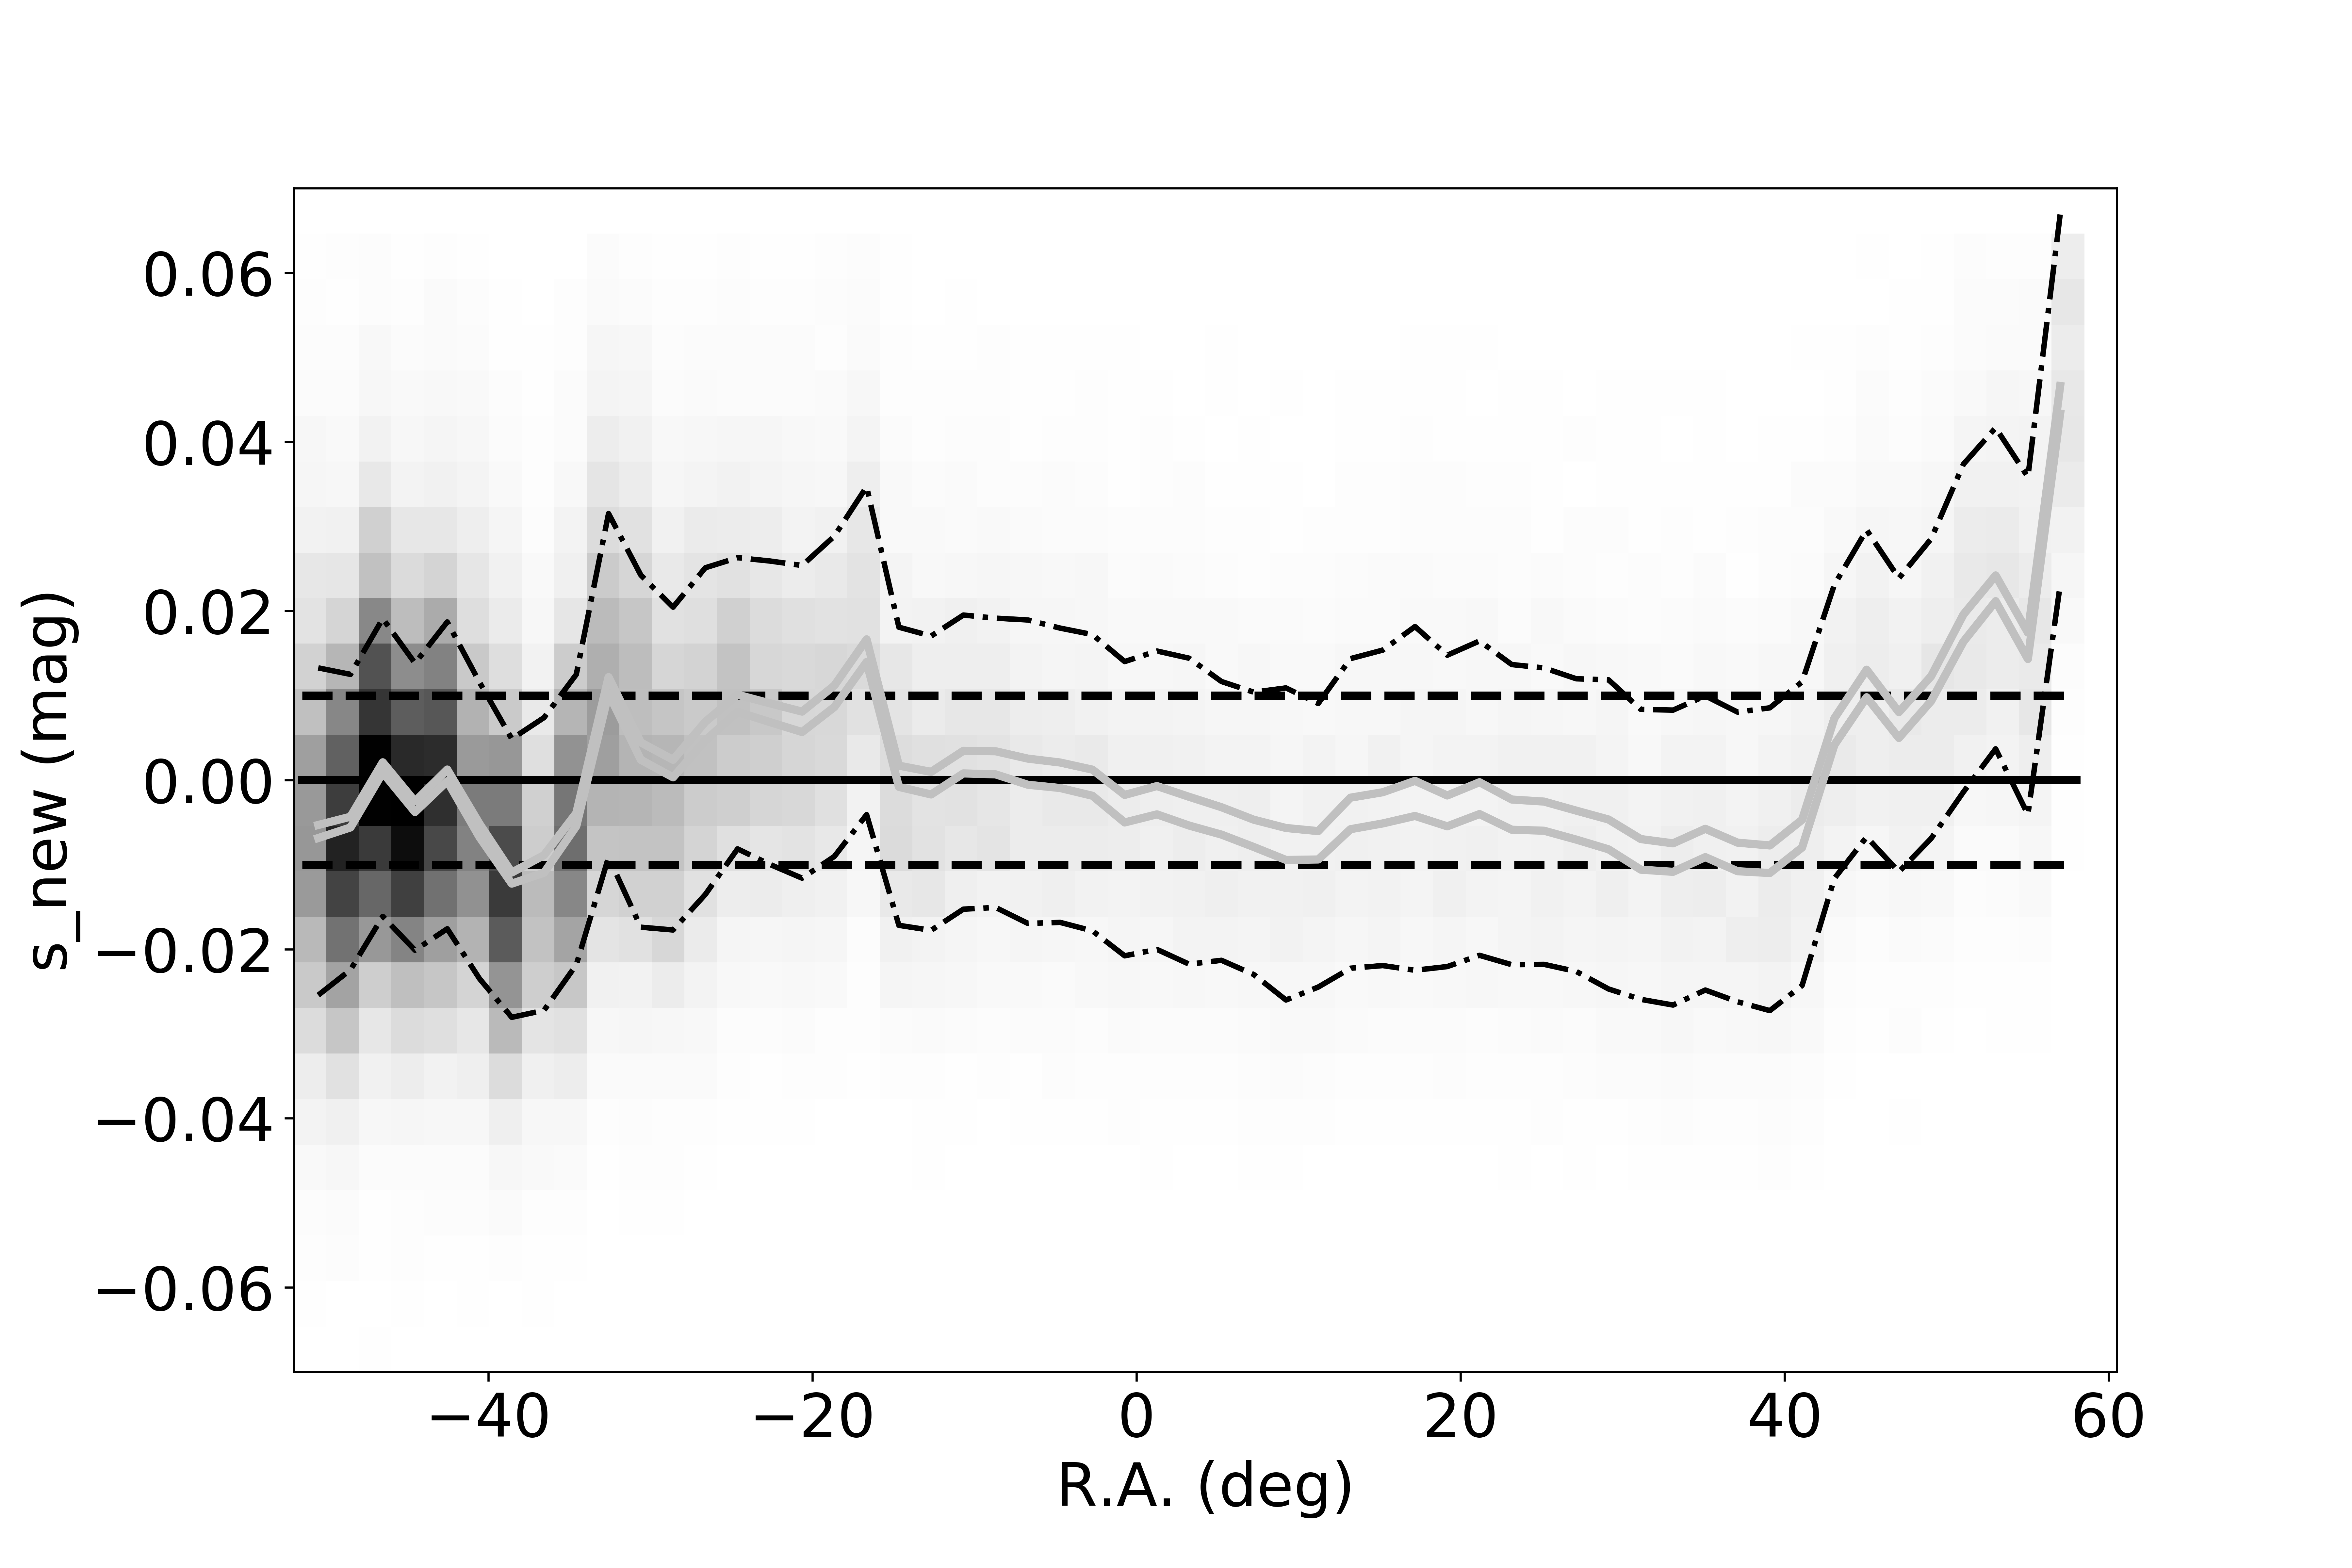
\includegraphics[width=7cm]{figures/testV26vsV33_snew_u_s_new_RA_Hess.png}
    \centering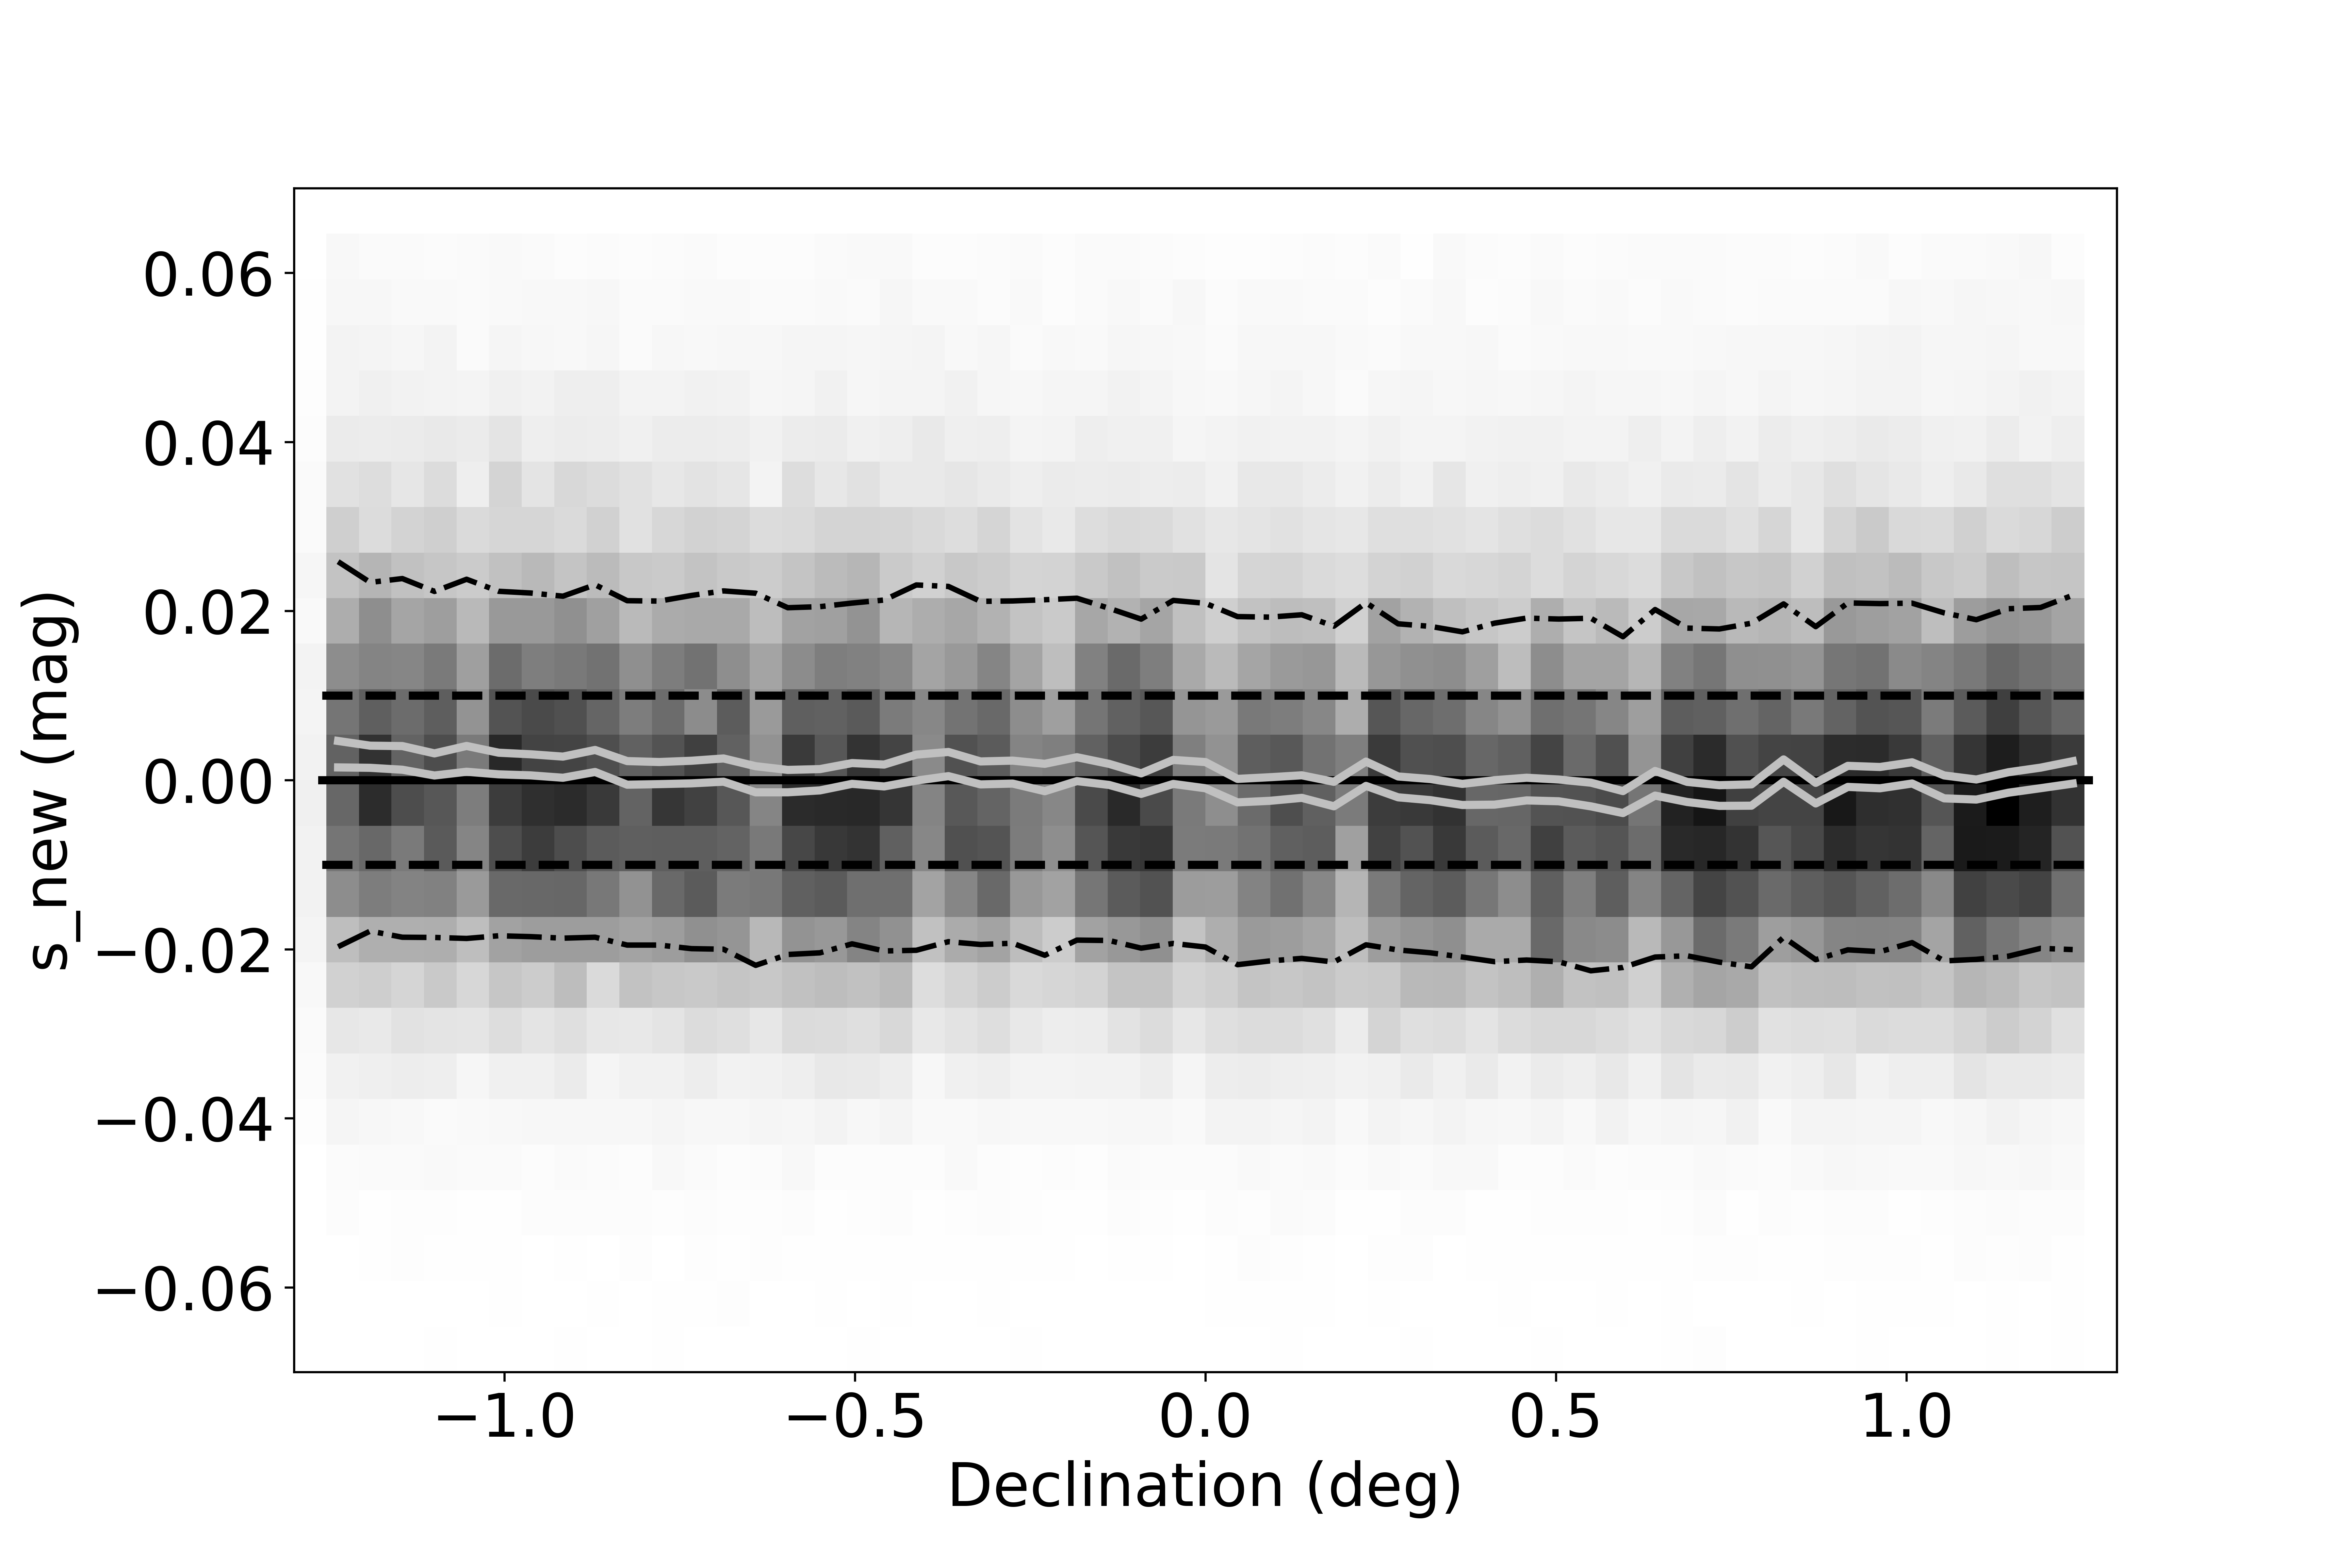
\includegraphics[width=7cm]{figures/testV26vsV33_snew_u_s_new_Dec_Hess.png} 
    \centering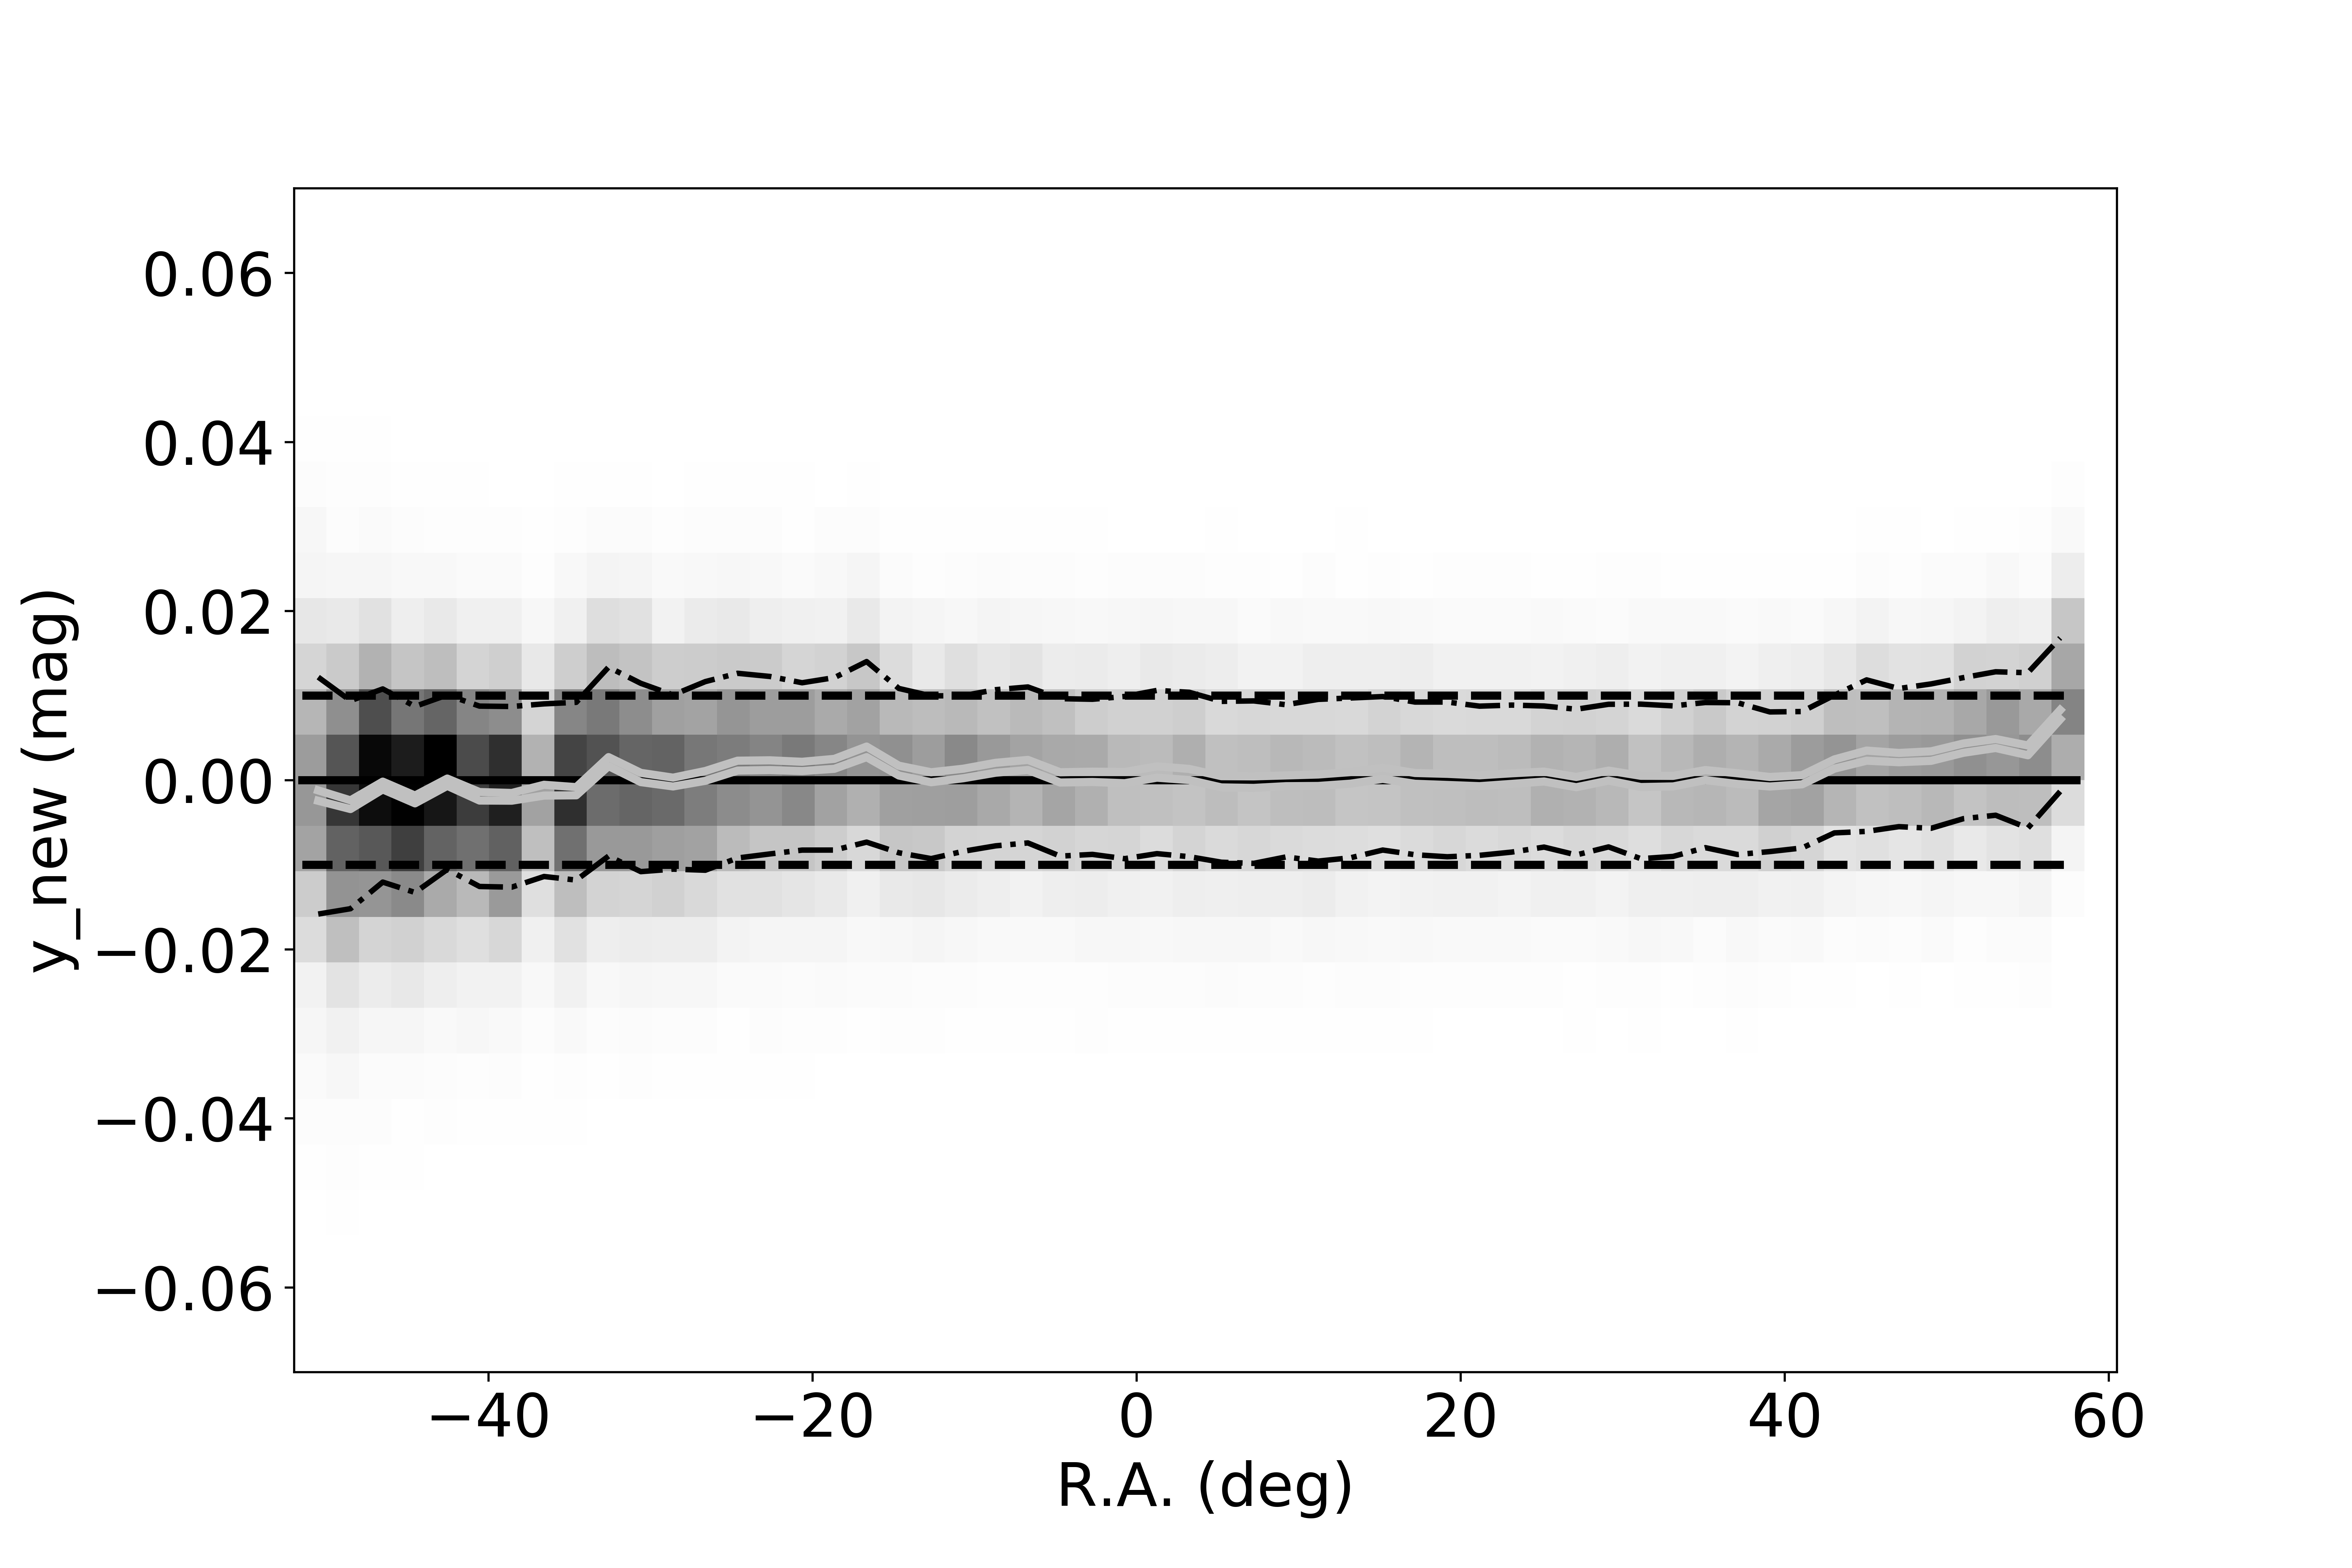
\includegraphics[width=7cm]{figures/testV26vsV33_ynew_z_y_new_RA_Hess.png} 
    \centering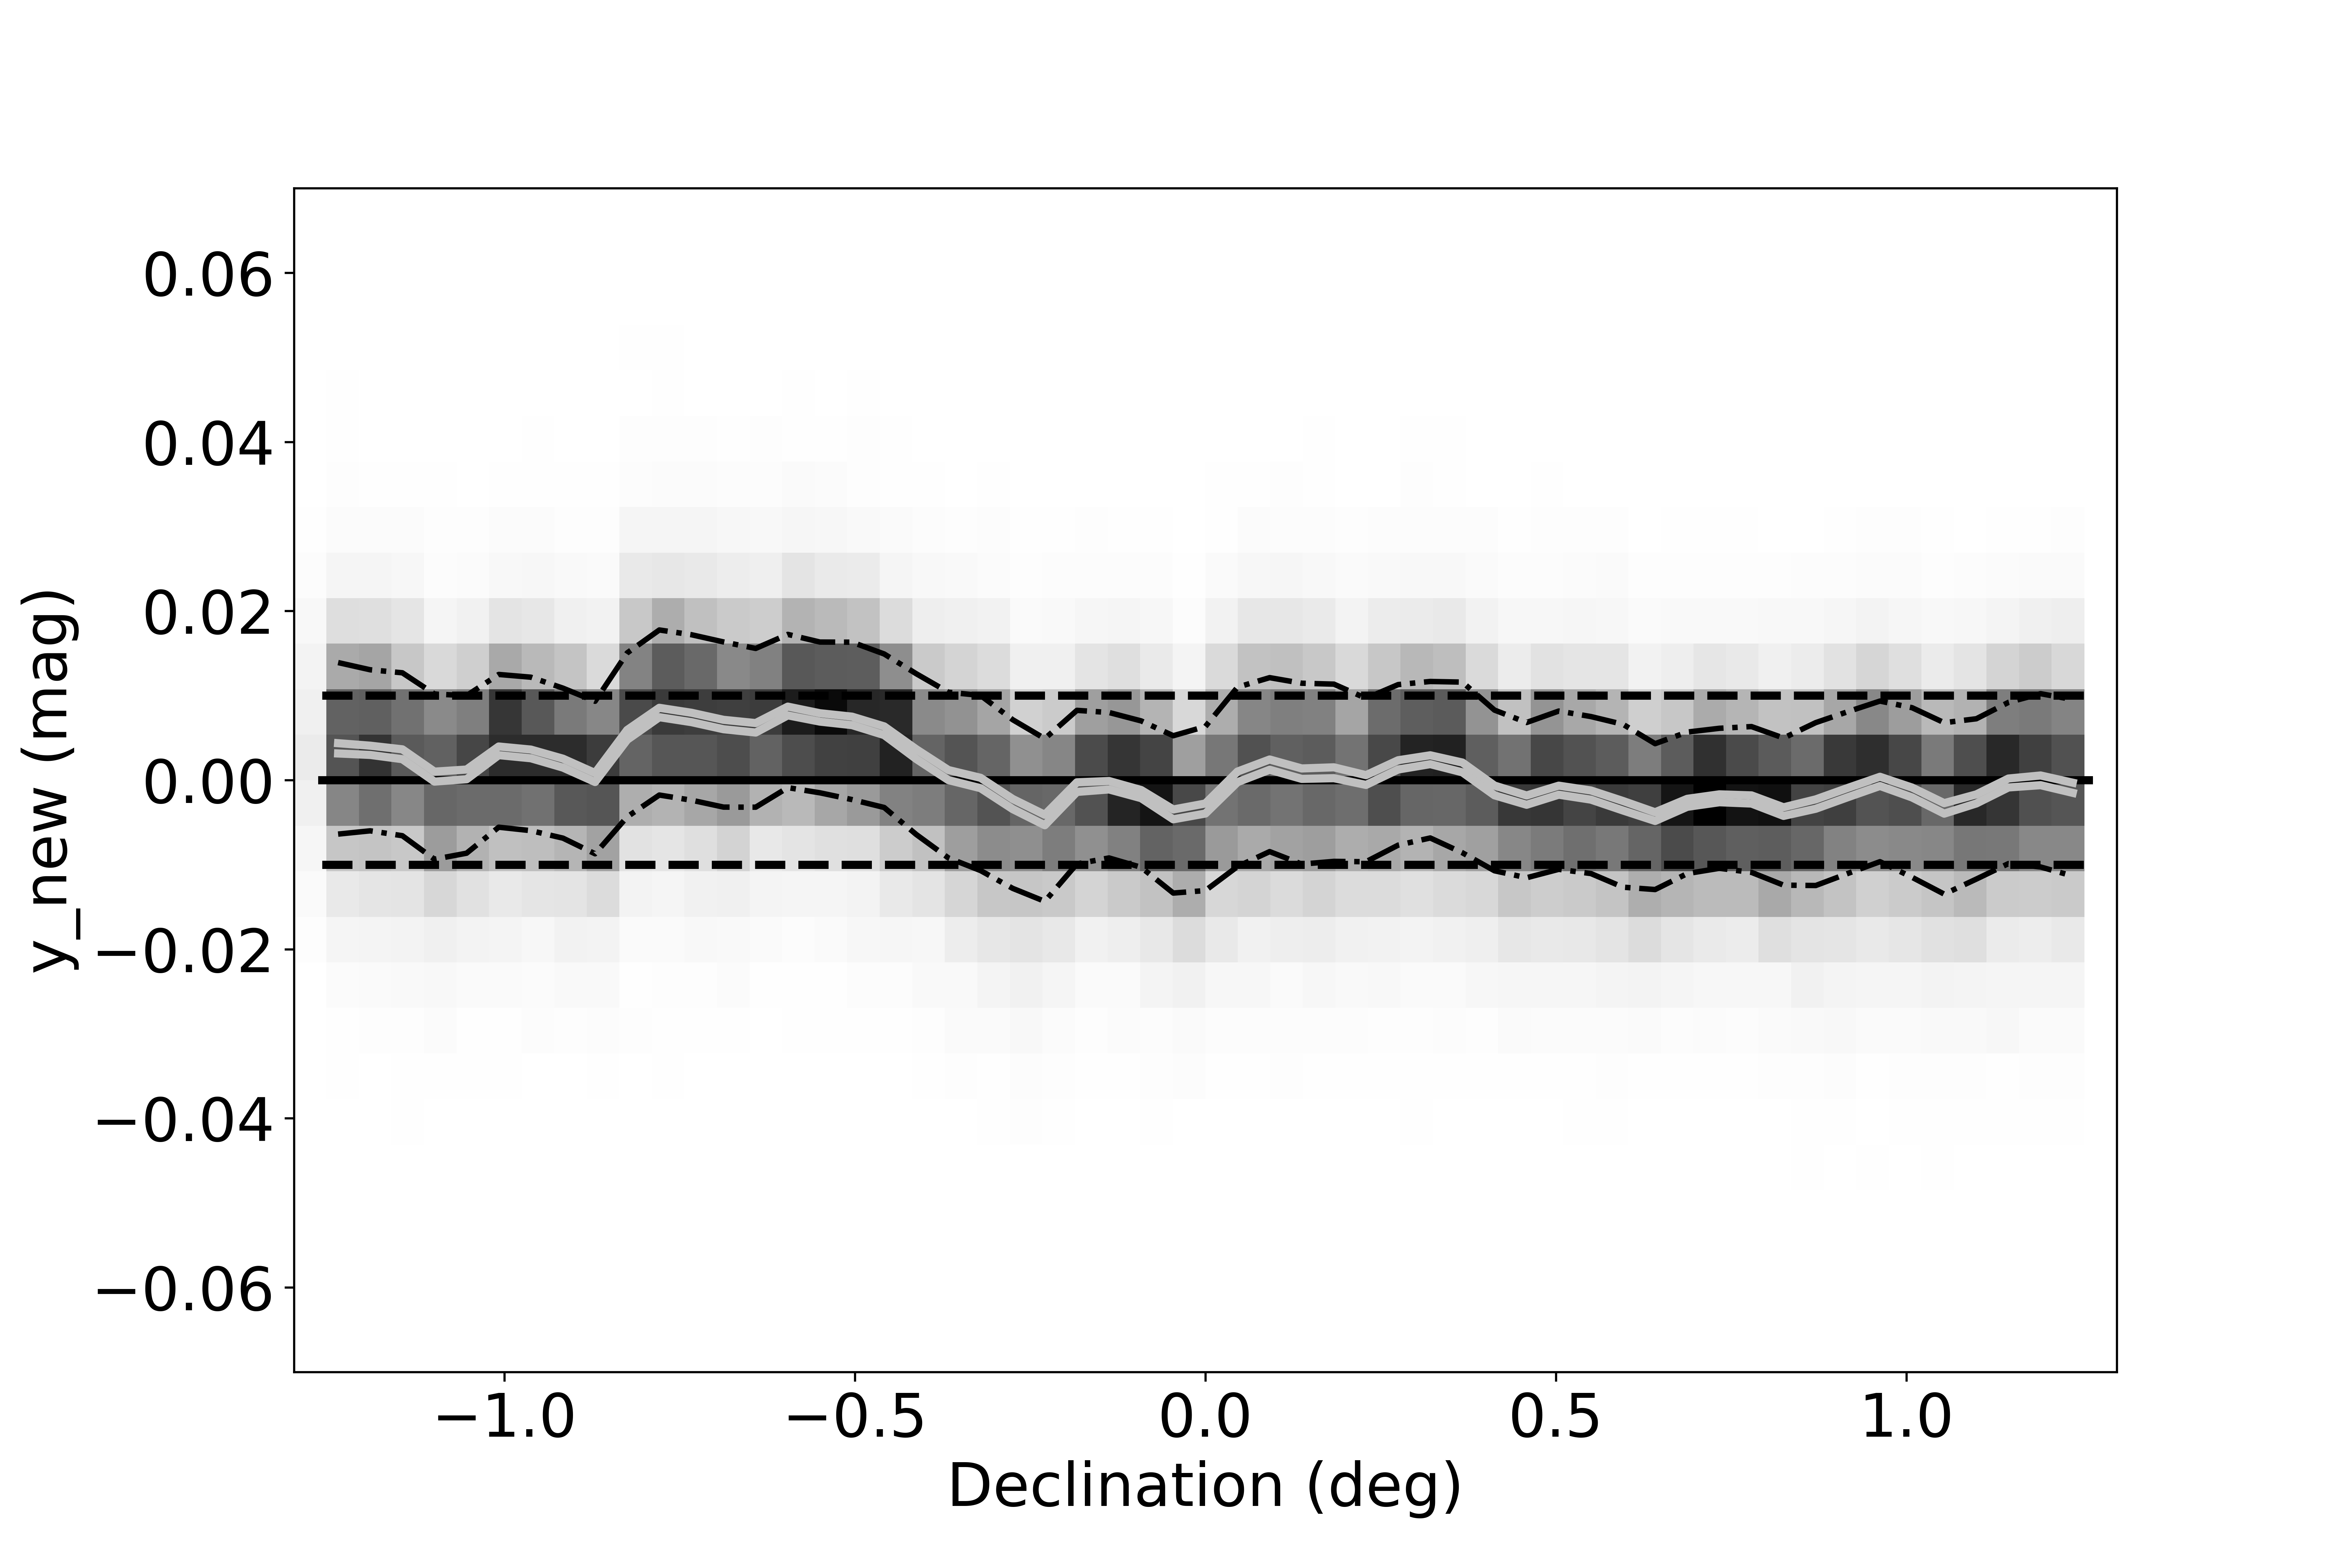
\includegraphics[width=7cm]{figures/testV26vsV33_ynew_z_y_new_Dec_Hess.png}  
\caption{The behavior of the $s$ color (top two panels), the second principal color in the SDSS
$g-r$ vs. $u-g$ color-color diagram, and the $y$ color (bottom two panels), the second 
principal color in the SDSS $i-z$ vs. $r-i$ color-color diagram, for the new v3.4 catalog.
The standard deviation of the median $s$ values binned by R.A. and Declination is 9.8 millimag 
and 1.3 millimag, respectively, and 1.8 millimag and 3.4 millimag for the $y$ color.}
\label{fig:comparesy} 
\end{figure}
  

\subsection{Comparison of the new v3.4 SDSS catalog with DES and Pan-STARRS catalogs \label{sec:DESPS1}} 
  
The quality of photometric zeropoint calibration for the new SDSS catalog can be conveniently
tested with the DES (see Section~\ref{ssec:des}) and Pan-STARRS (see Section~\ref{ssec:ps1}) catalogs. 
Both catalogs list $griz$ photometry of sufficient precision for esentially all stars
from Stripe 82. Their photometric calibration procedures are expected to result in different 
spatial patterns and thus a cross-comparison with the v3.4 catalog can reveal residual problems
with zeropoint calibration. They are also deeper than Gaia DR2 catalog and thus can provide
further clues about the Gmag discrepancy at Gaia's faint end illustrated in Figure~\ref{fig:gaiaJump}. 

Our comparison of the magnitude differences is illustrated in Figures~\ref{fig:DESPSRA} and \ref{fig:DESPSDec},
and the robust standard deviation for binned median magnitude differences is listed in Table~\ref{tab:DESPS1}. 
This multi-survey comparison indicates that the spatial variation of photometric zero points in the 
updated SDSS catalog is well below 0.01 mag (rms), with typical values of 3-7 millimag in the R.A. 
direction and 1-2 millimag in the Declination direction. As discernible in the two bottom panels
in Figure~\ref{fig:DESPSRA}, there are systematic residual errors in the $z$ band zeropoint as a 
function of  Declination at the level of a few millimag. Note also implied DES $z$ band zeropoint errors 
of up to 0.01-0.02 mag, as a function of R.A. (see the bottom left panel in Figure~\ref{fig:DESPSRA}). 

The variation of the magnitude differences
with magnitude (see Figure~\ref{fig:drVSr}) shows good agreement (to within $\sim$5 millimag) 
even at the faint end ($20<r<21$), where Gaia Gmag magnitudes appear too faint by about
0.02 mag, and thus demonstrates a likely problem with Gaia DR2 photometry. 
 
\begin{deluxetable}{l|c|c|c|c}[ht!]
\tablecaption{The robust standard deviation for binned median magnitude differences between
the new v3.4 SDSS catalog, and DES and Pan-STARRS1 (PS1) catalogs (millimag). \label{tab:DESPS1}}
\tablehead{
\colhead{Band} & \colhead{DES R.A.} & \colhead{DES Dec} & \colhead{PS1 R.A.} & \colhead{PS1 Dec} 
}
\startdata
       $g$        &        5.1    &      1.8   &        3.4    &      1.4        \\
       $r$         &        4.1    &      0.8   &        2.6    &      0.7         \\  
       $i$         &        7.3    &      1.6   &        3.2    &      1.0         \\ 
       $z$        &       13.6    &     3.6   &        6.8    &      2.3         \\ 
\enddata
\end{deluxetable}
   

\begin{figure}[th!]
    \centering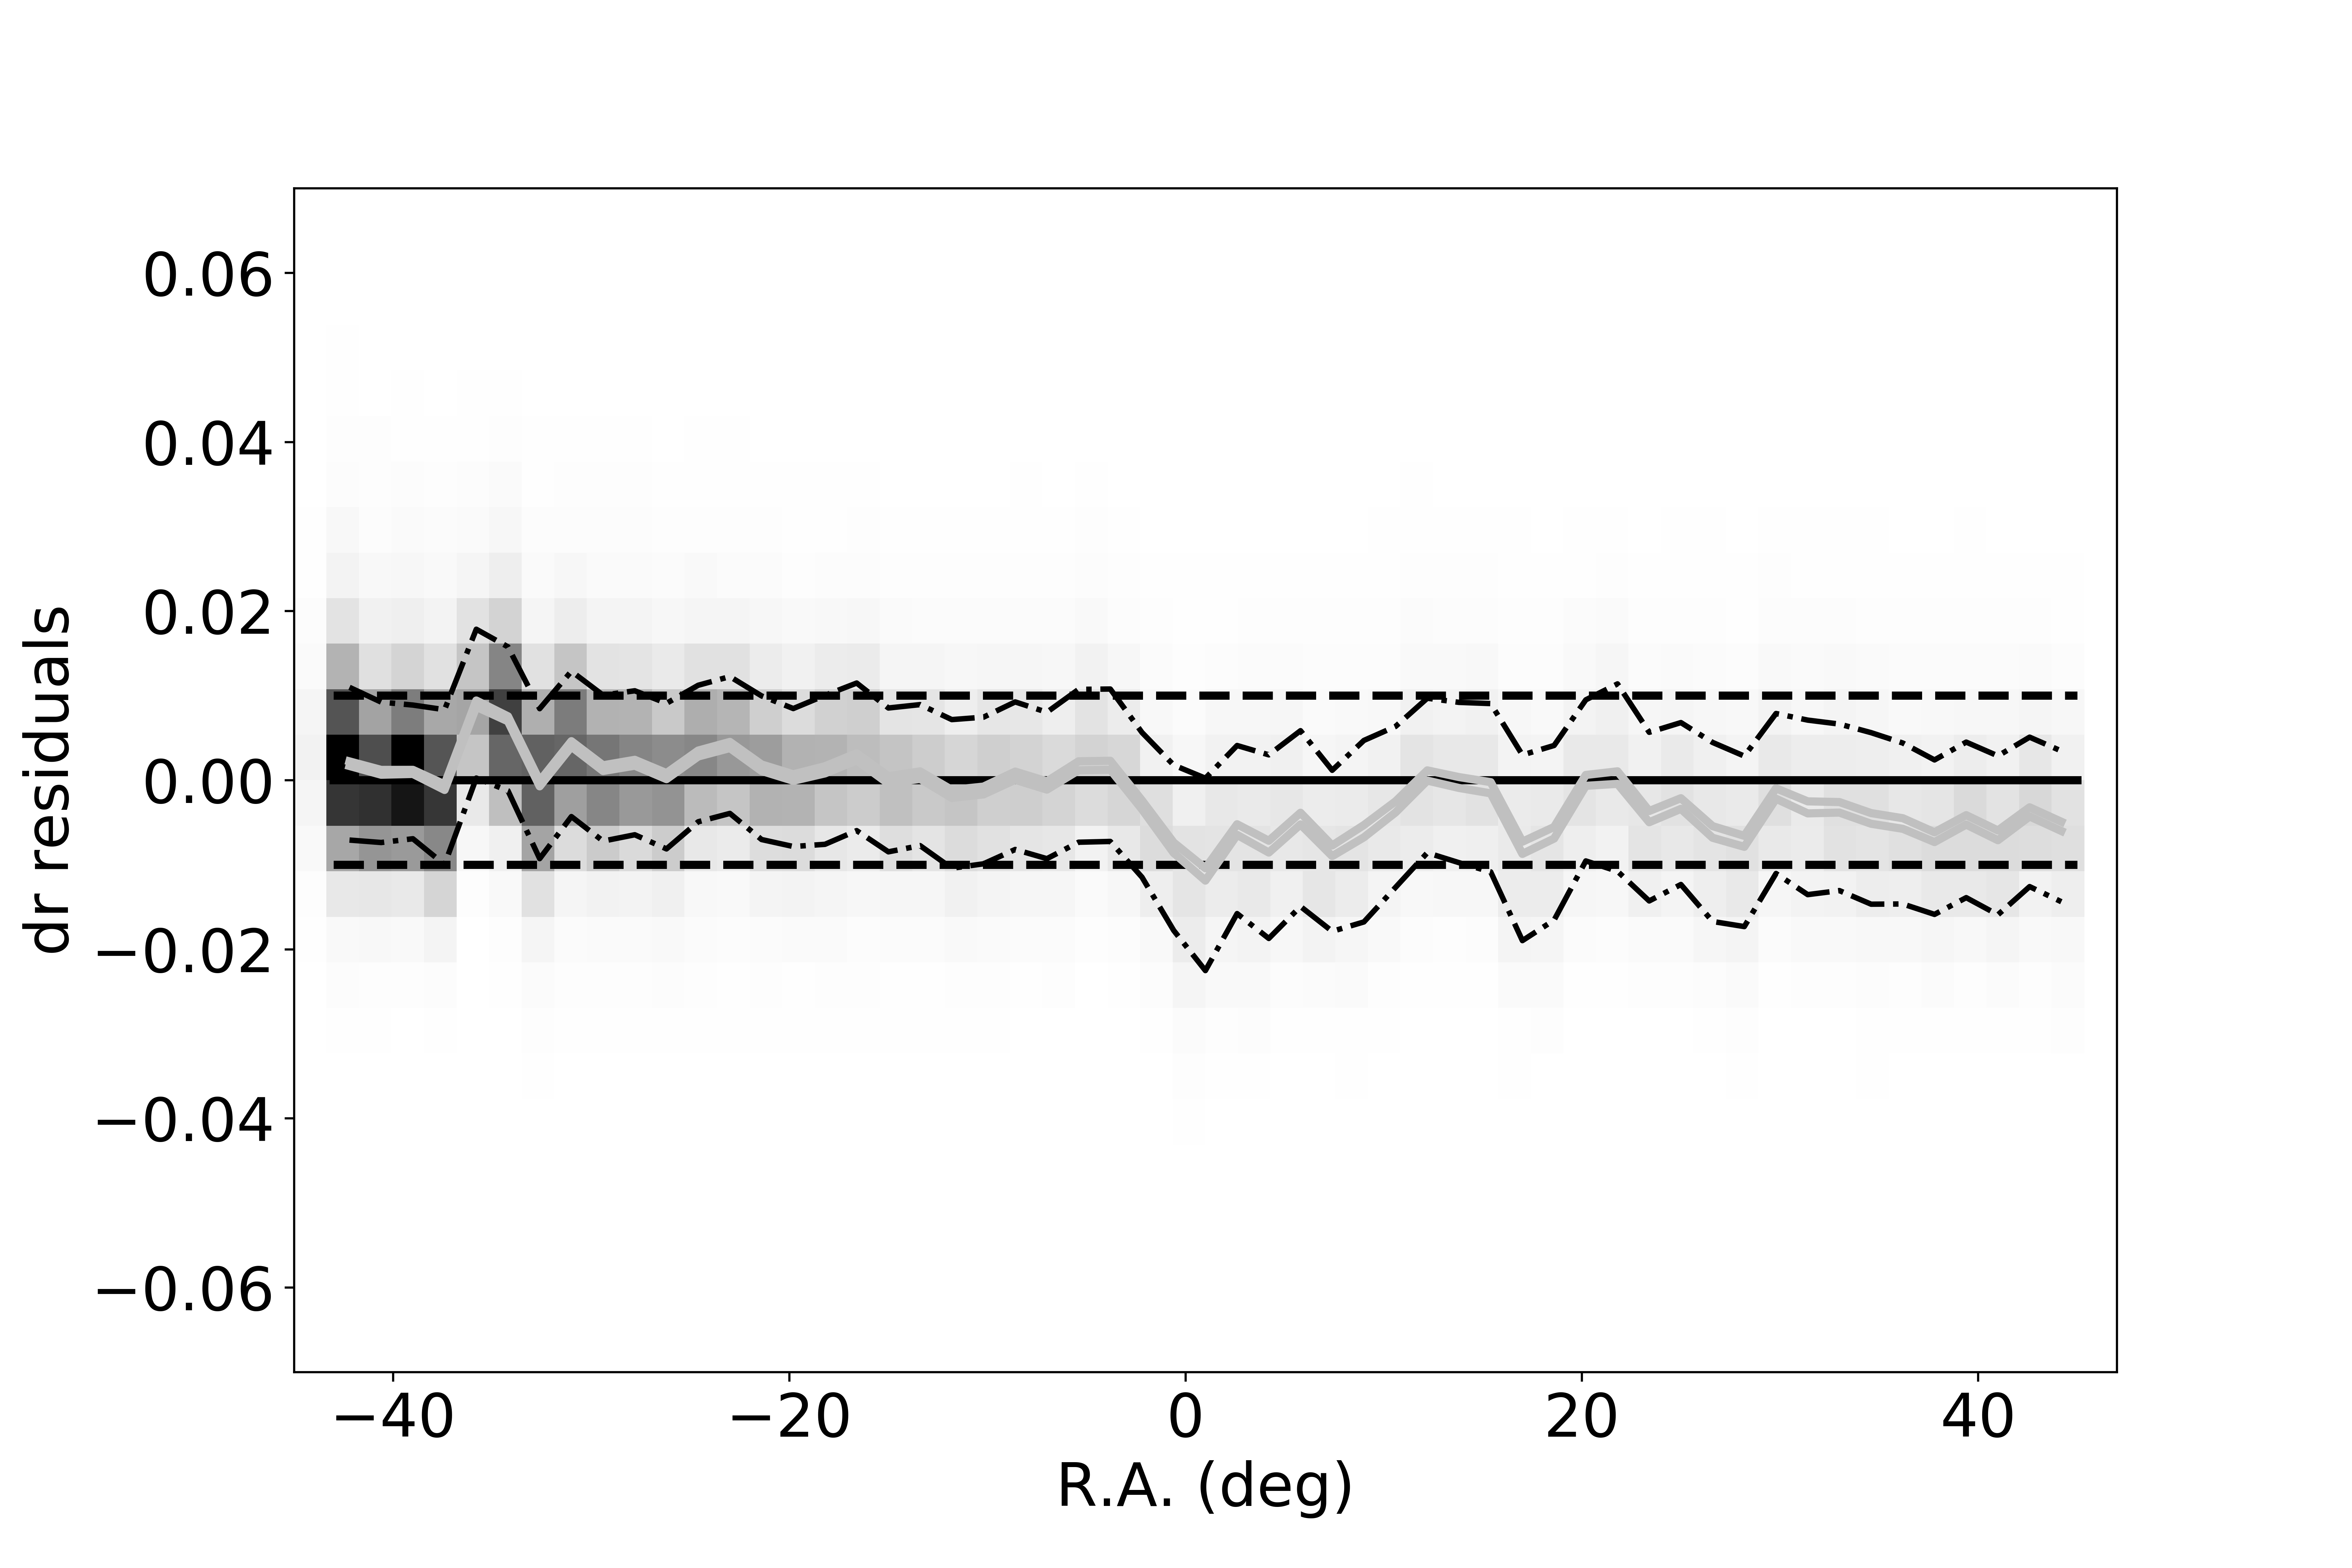
\includegraphics[width=7cm]{figures/colorResidDES2bright_dr_RA_Hess.png}
    \centering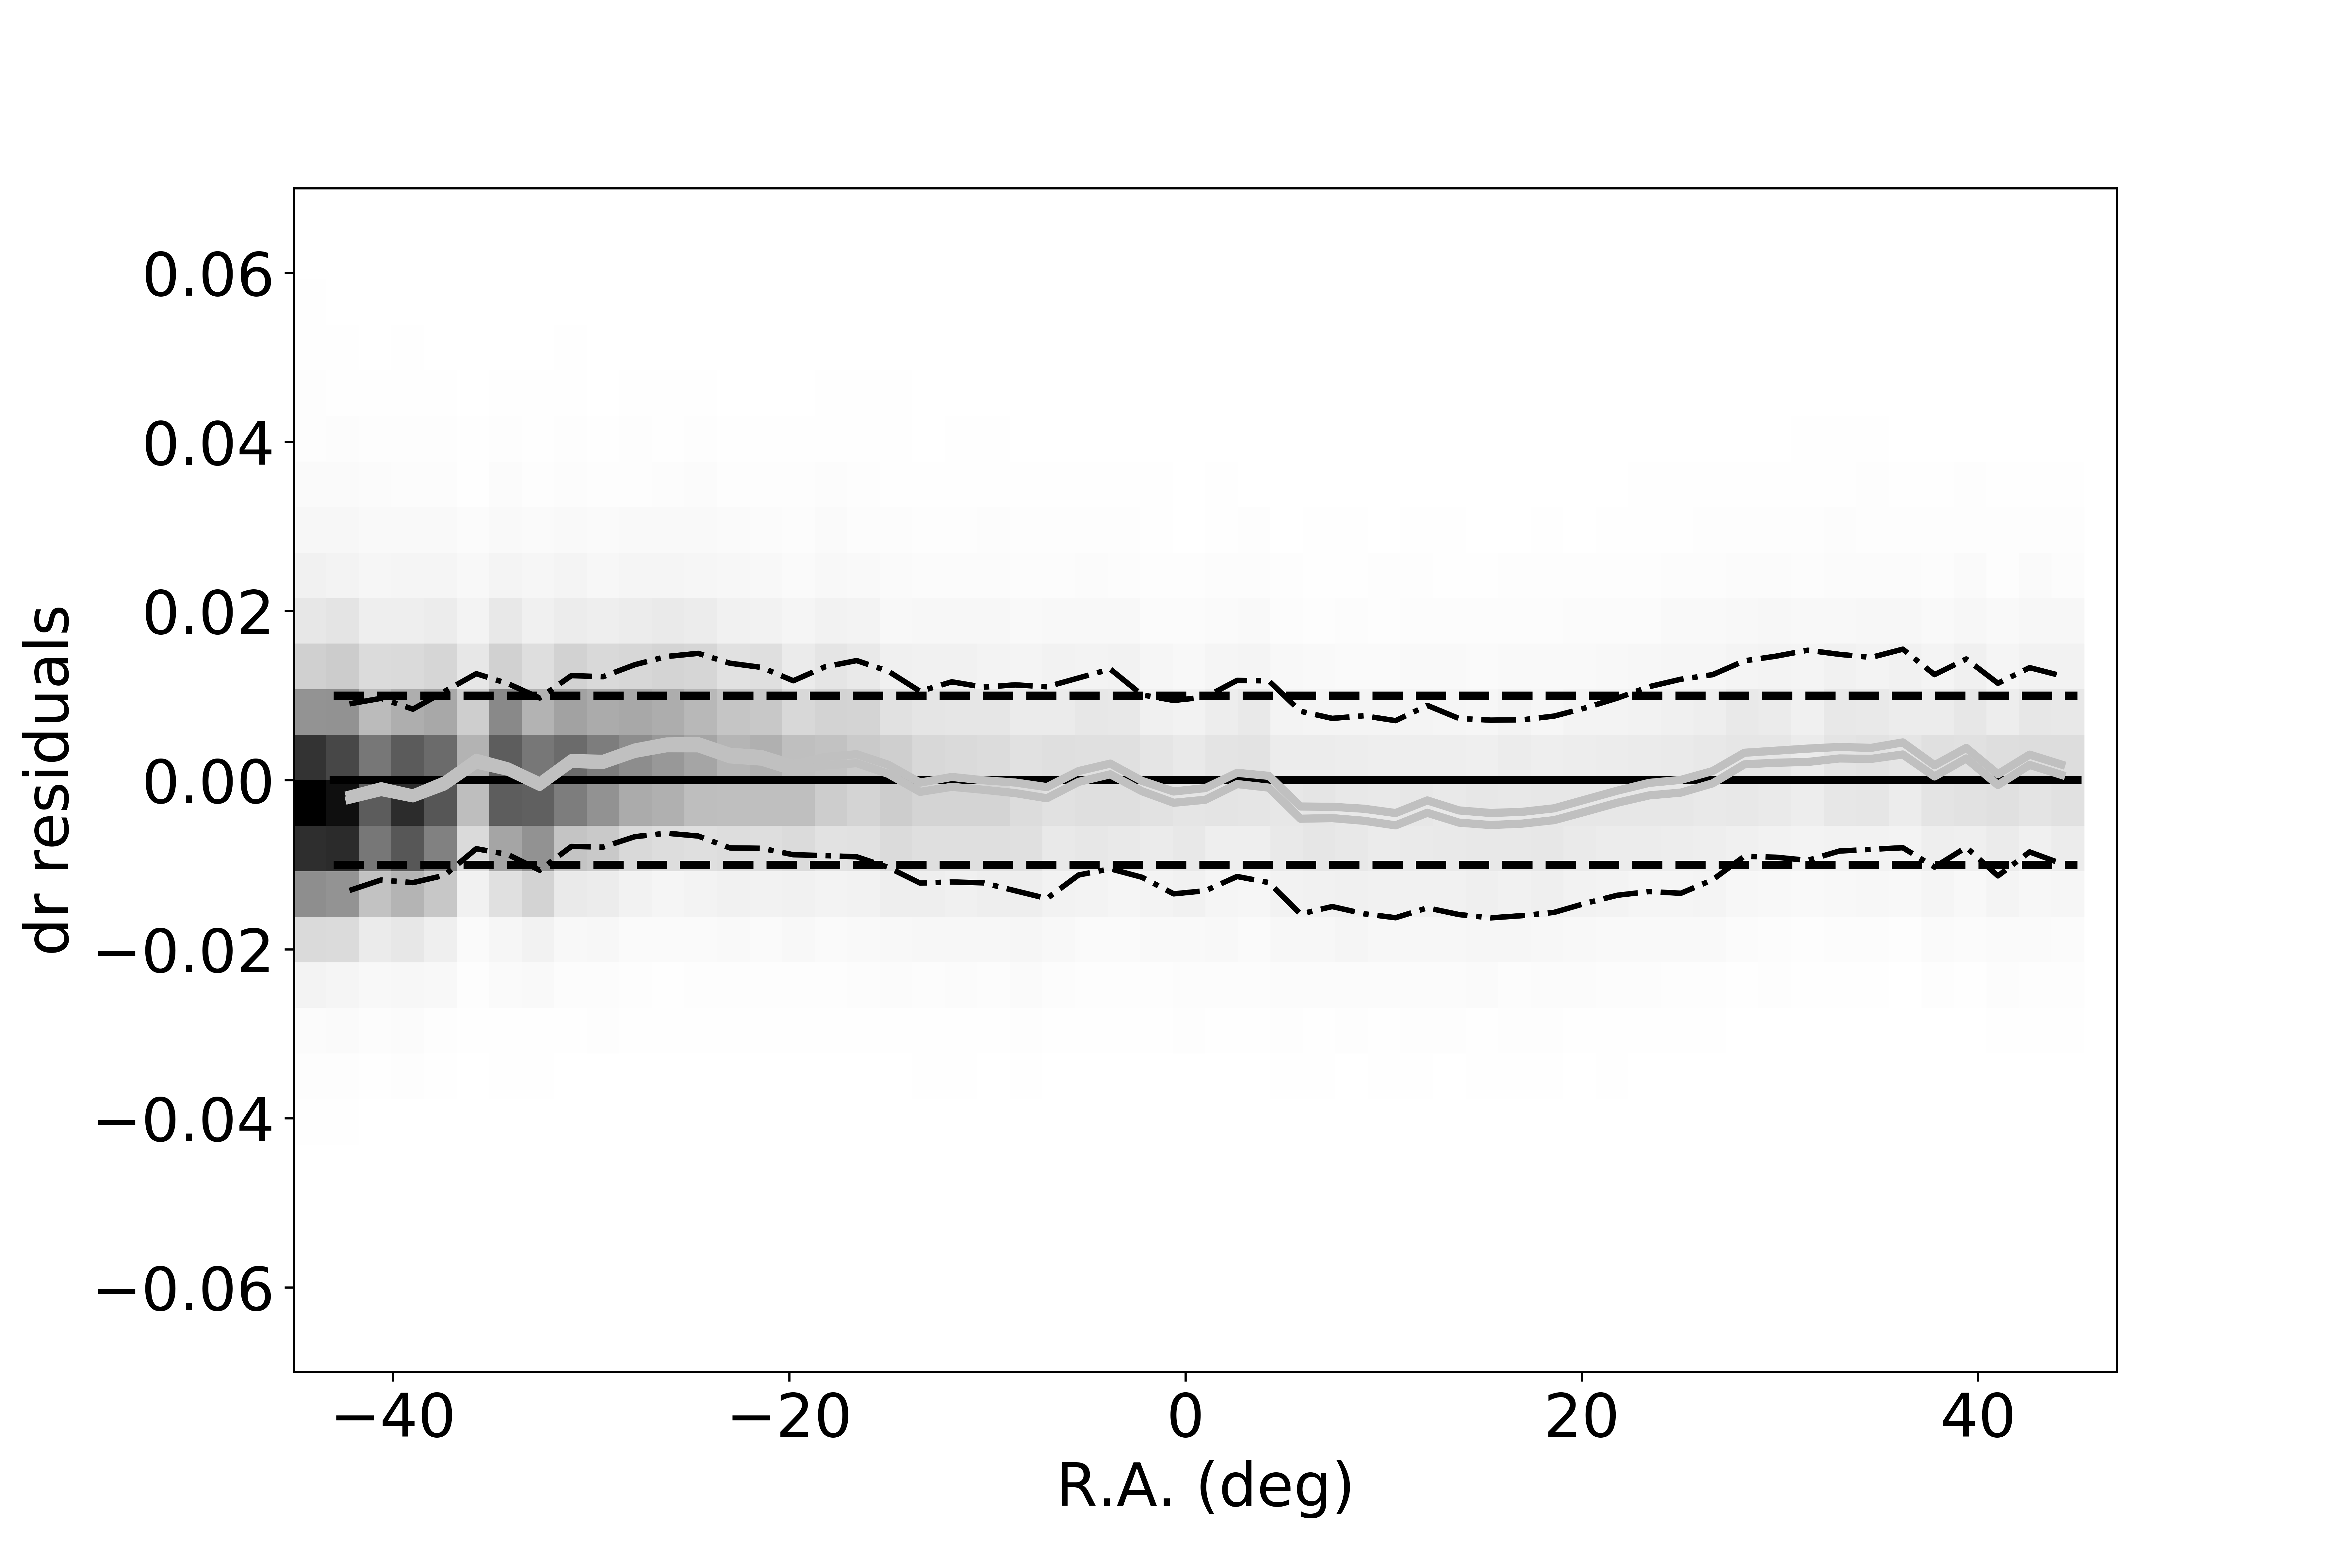
\includegraphics[width=7cm]{figures/colorResidPSbright_dr_RA_Hess.png}
    \centering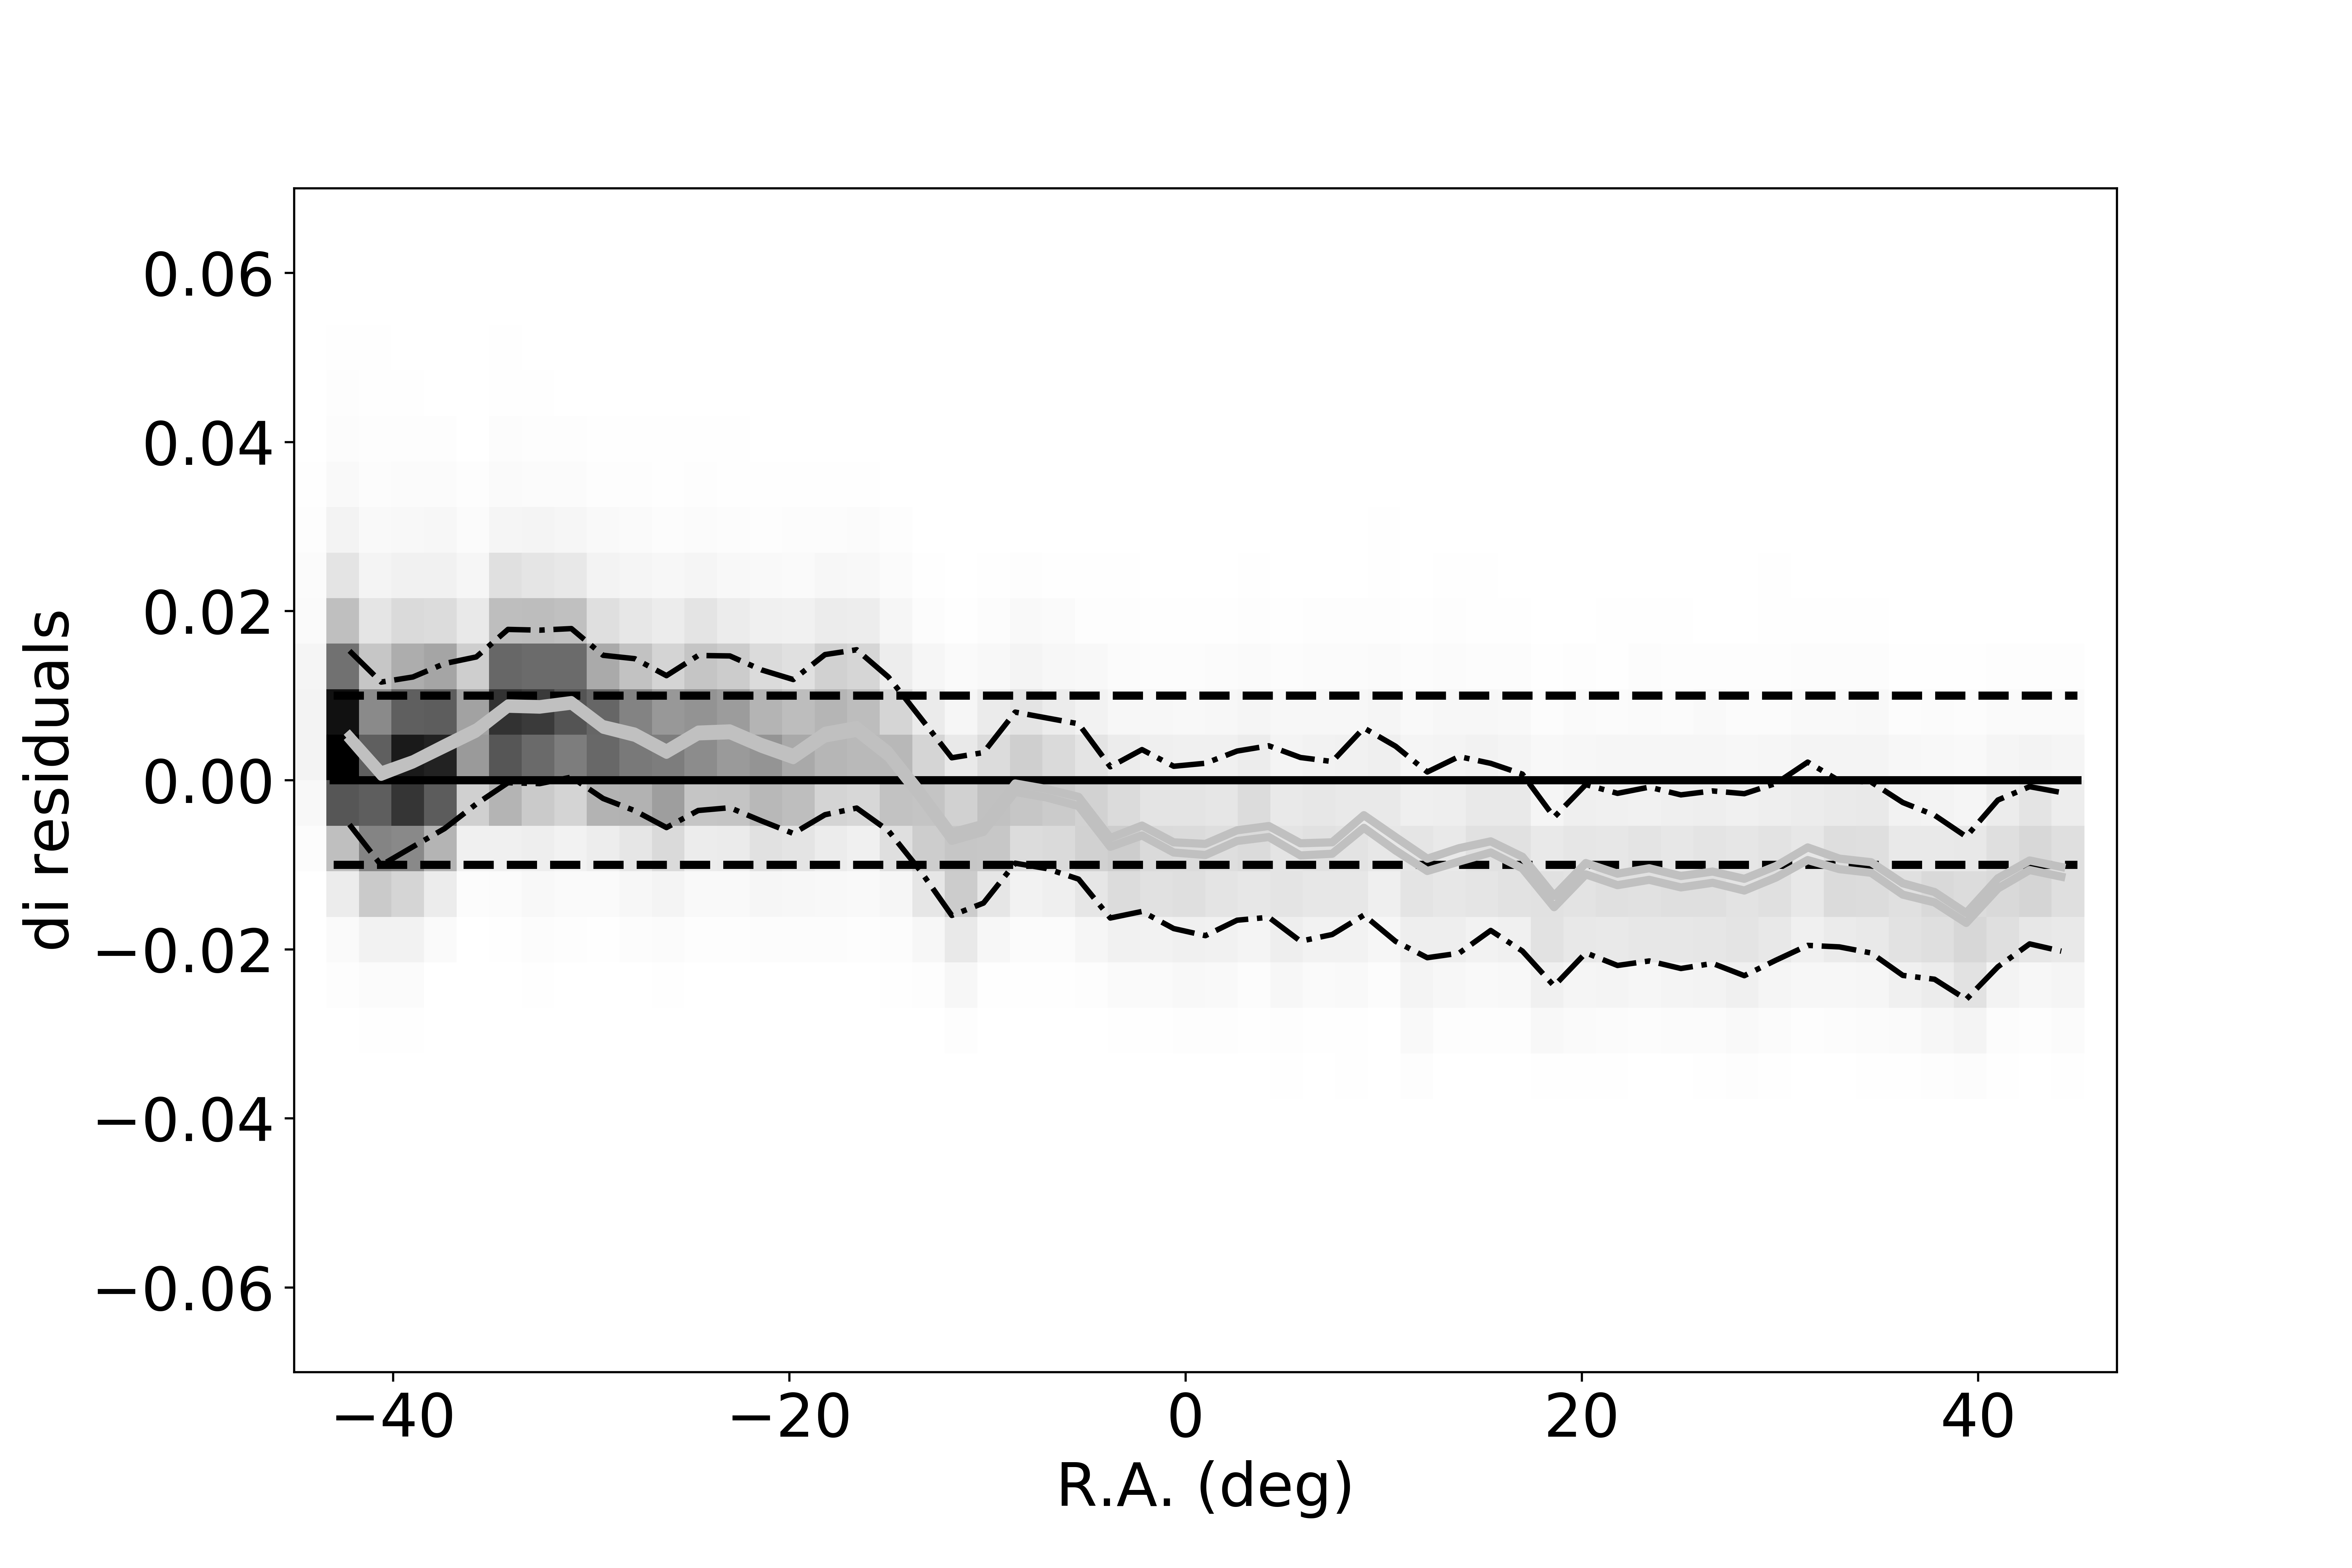
\includegraphics[width=7cm]{figures/colorResidDES2bright_di_RA_Hess.png}
    \centering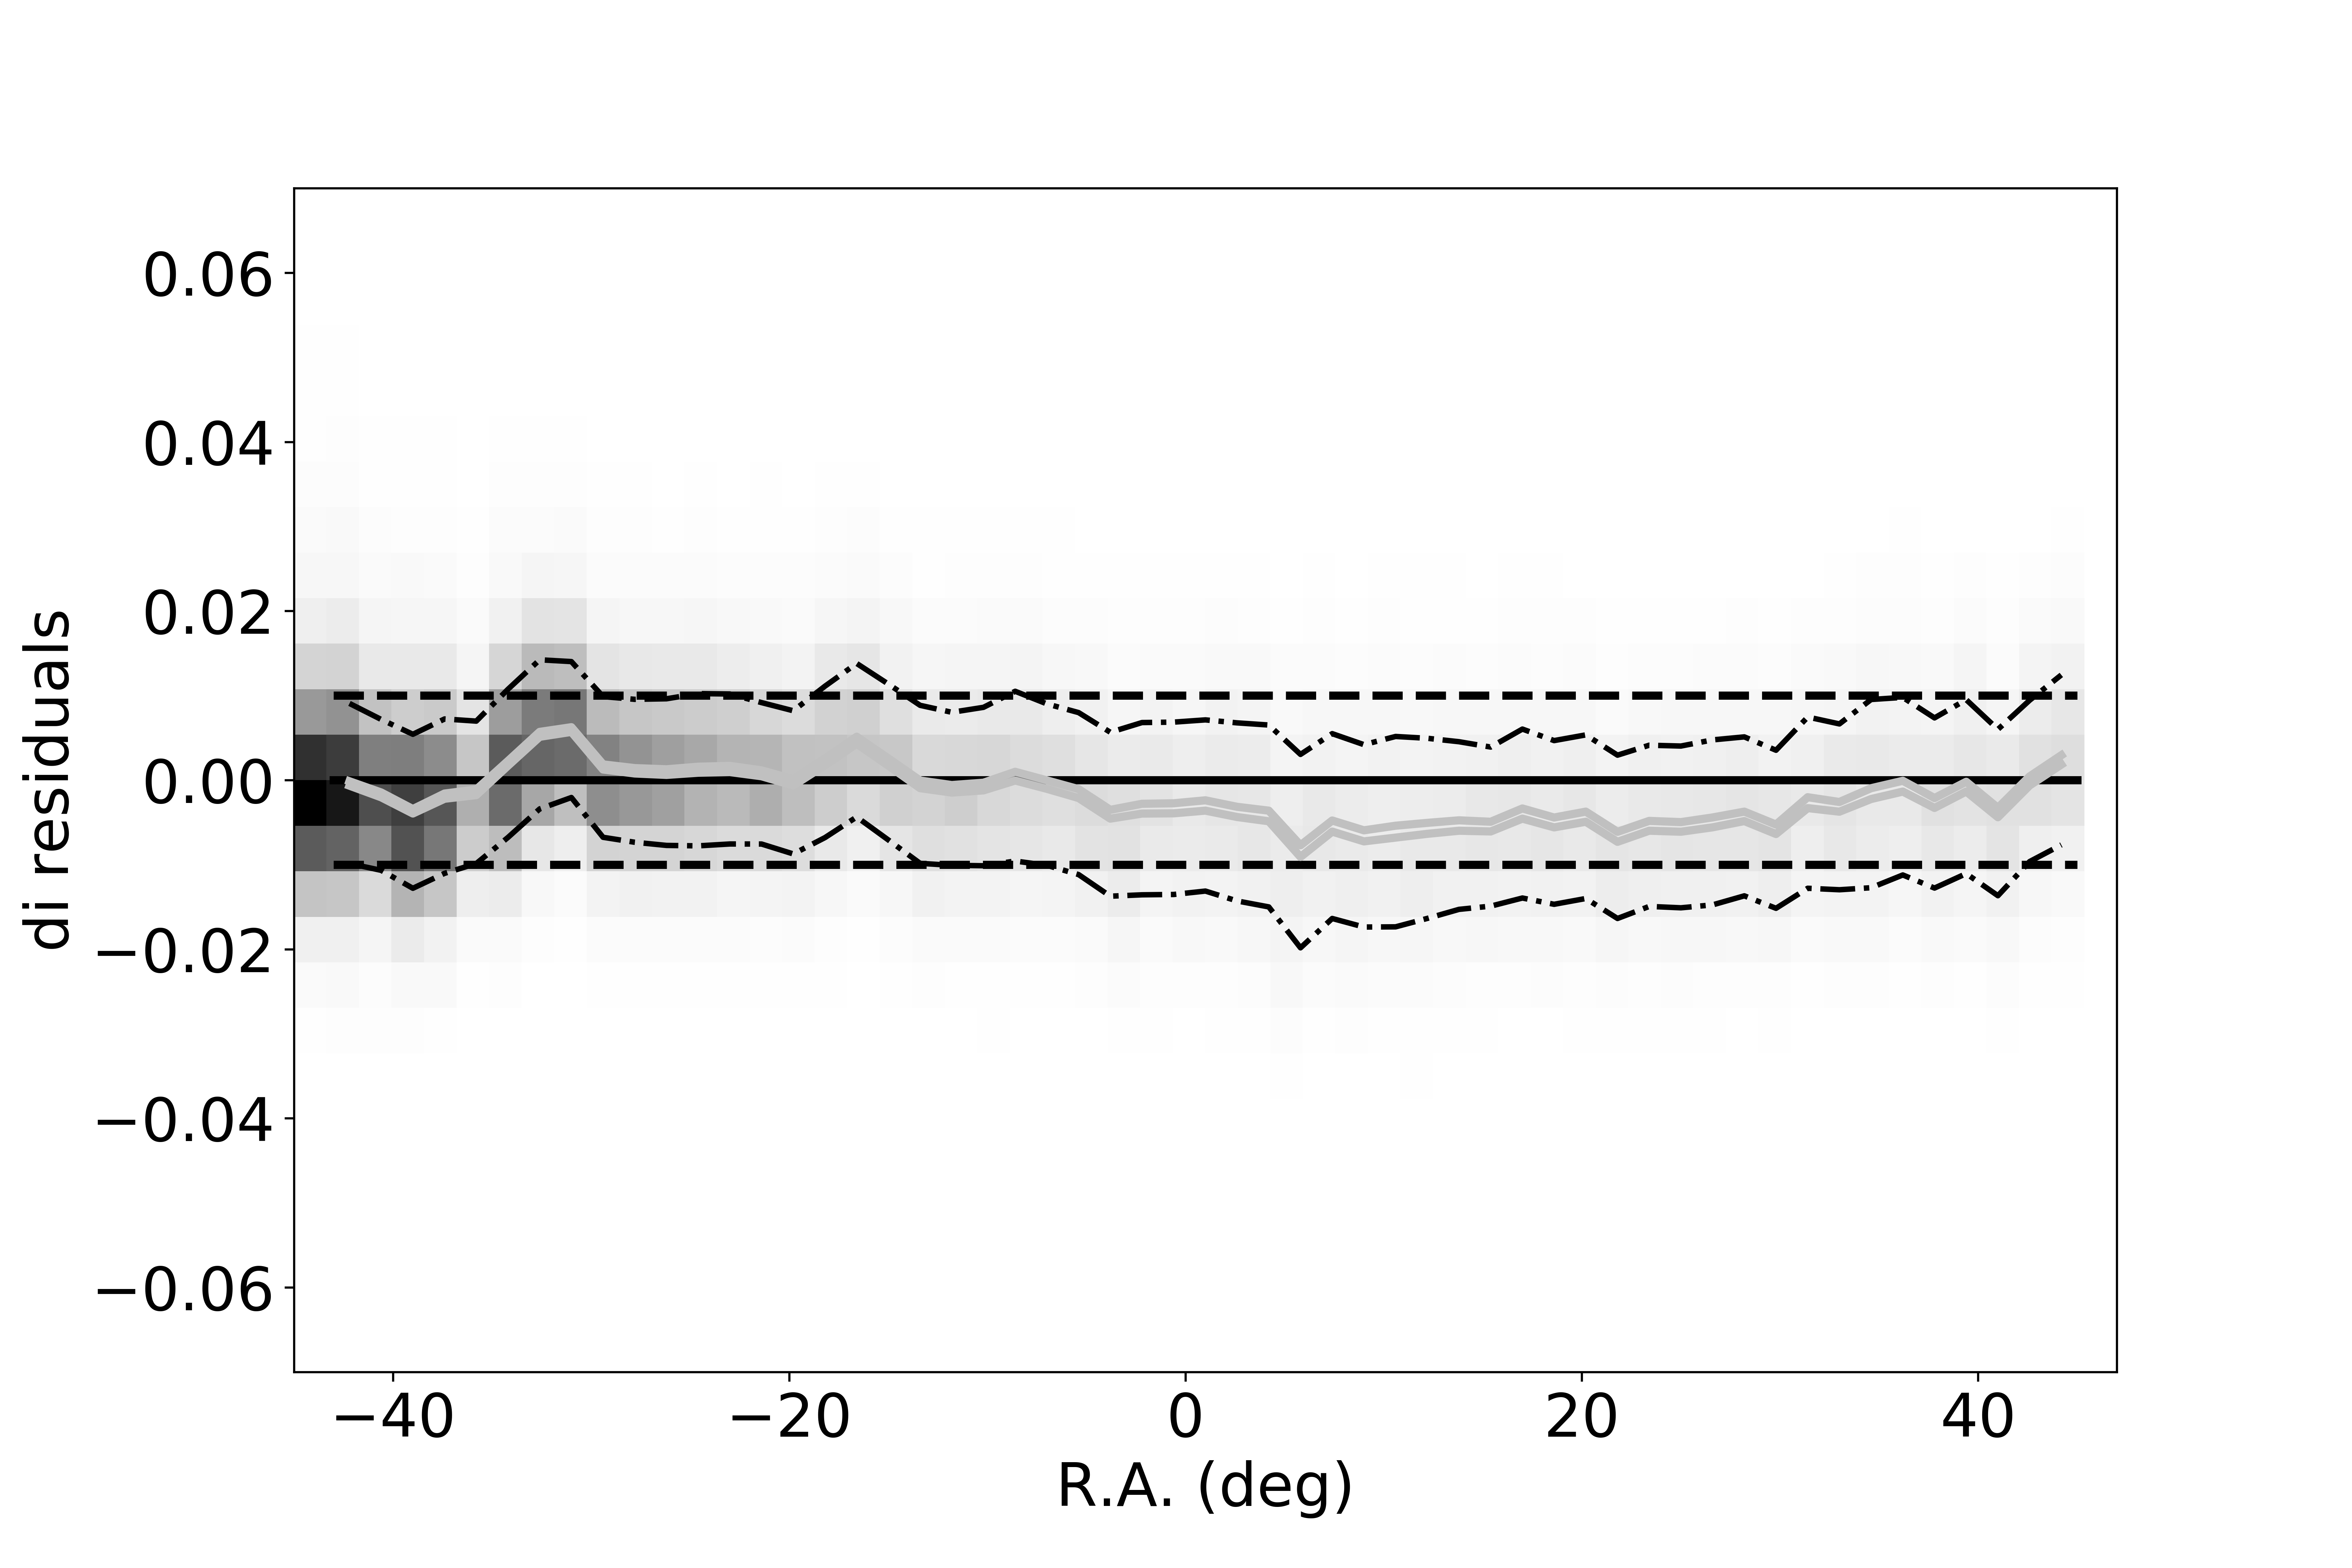
\includegraphics[width=7cm]{figures/colorResidPSbright_di_RA_Hess.png}
    \centering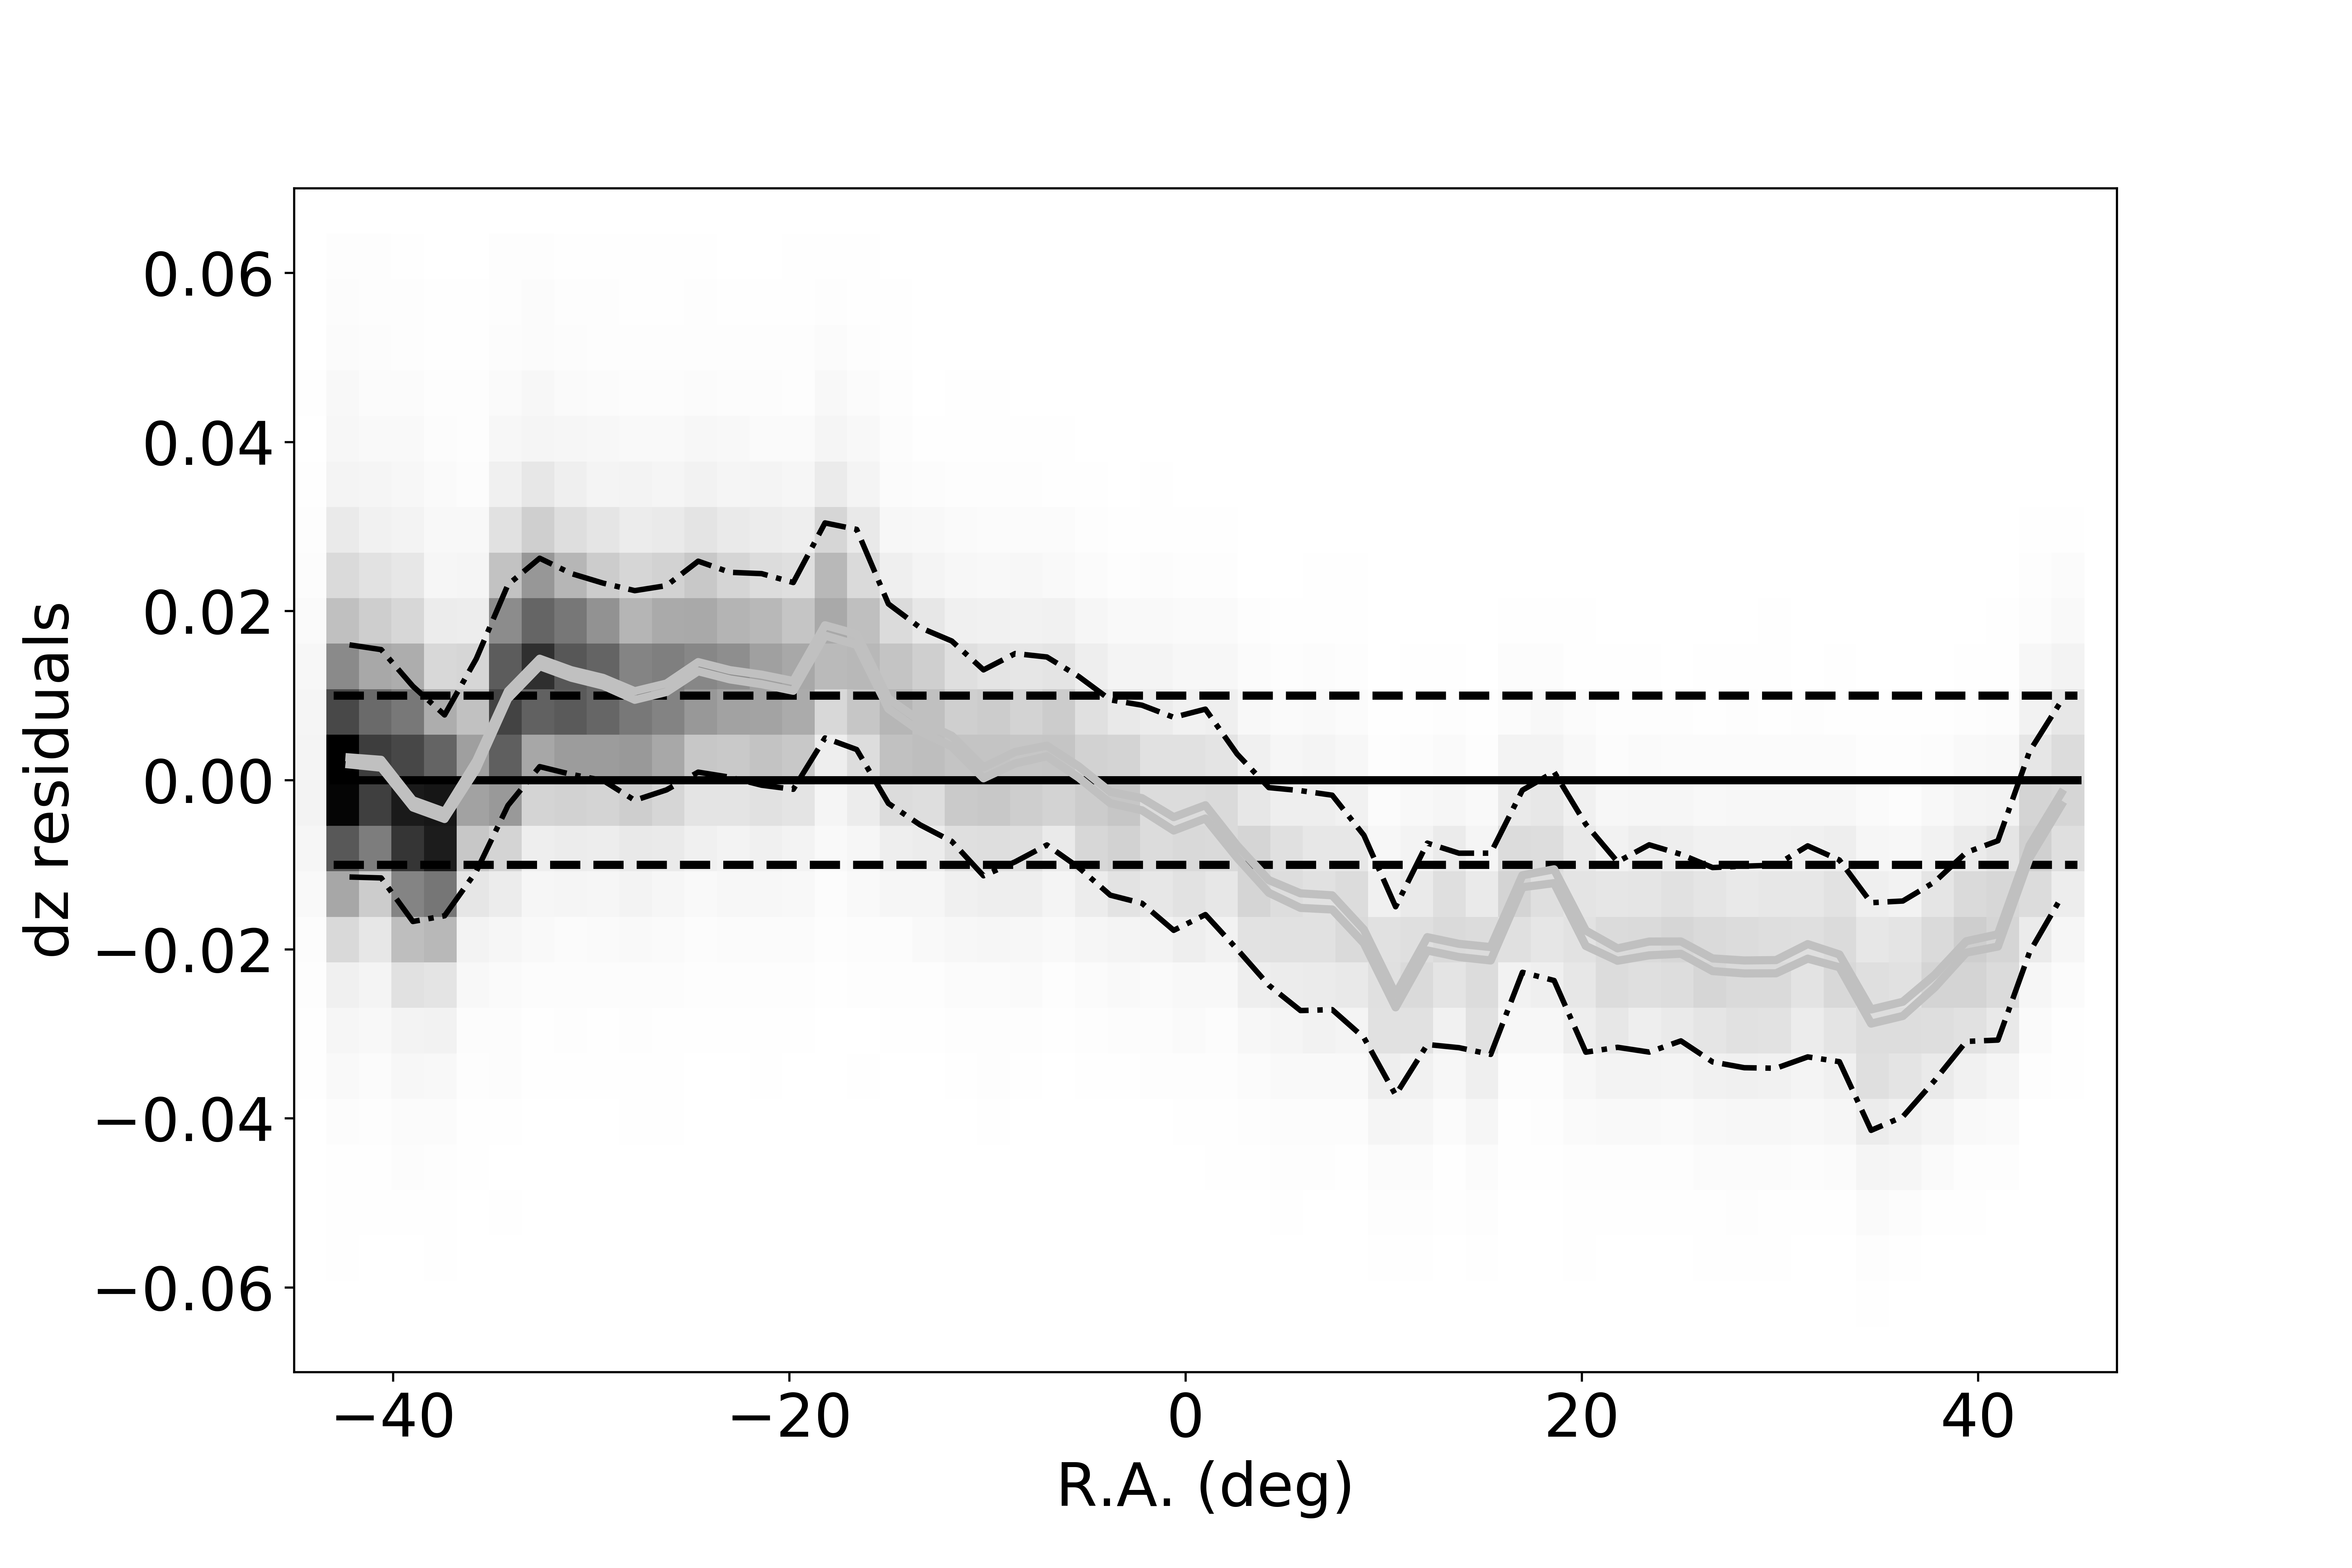
\includegraphics[width=7cm]{figures/colorResidDES2bright_dz_RA_Hess.png}
    \centering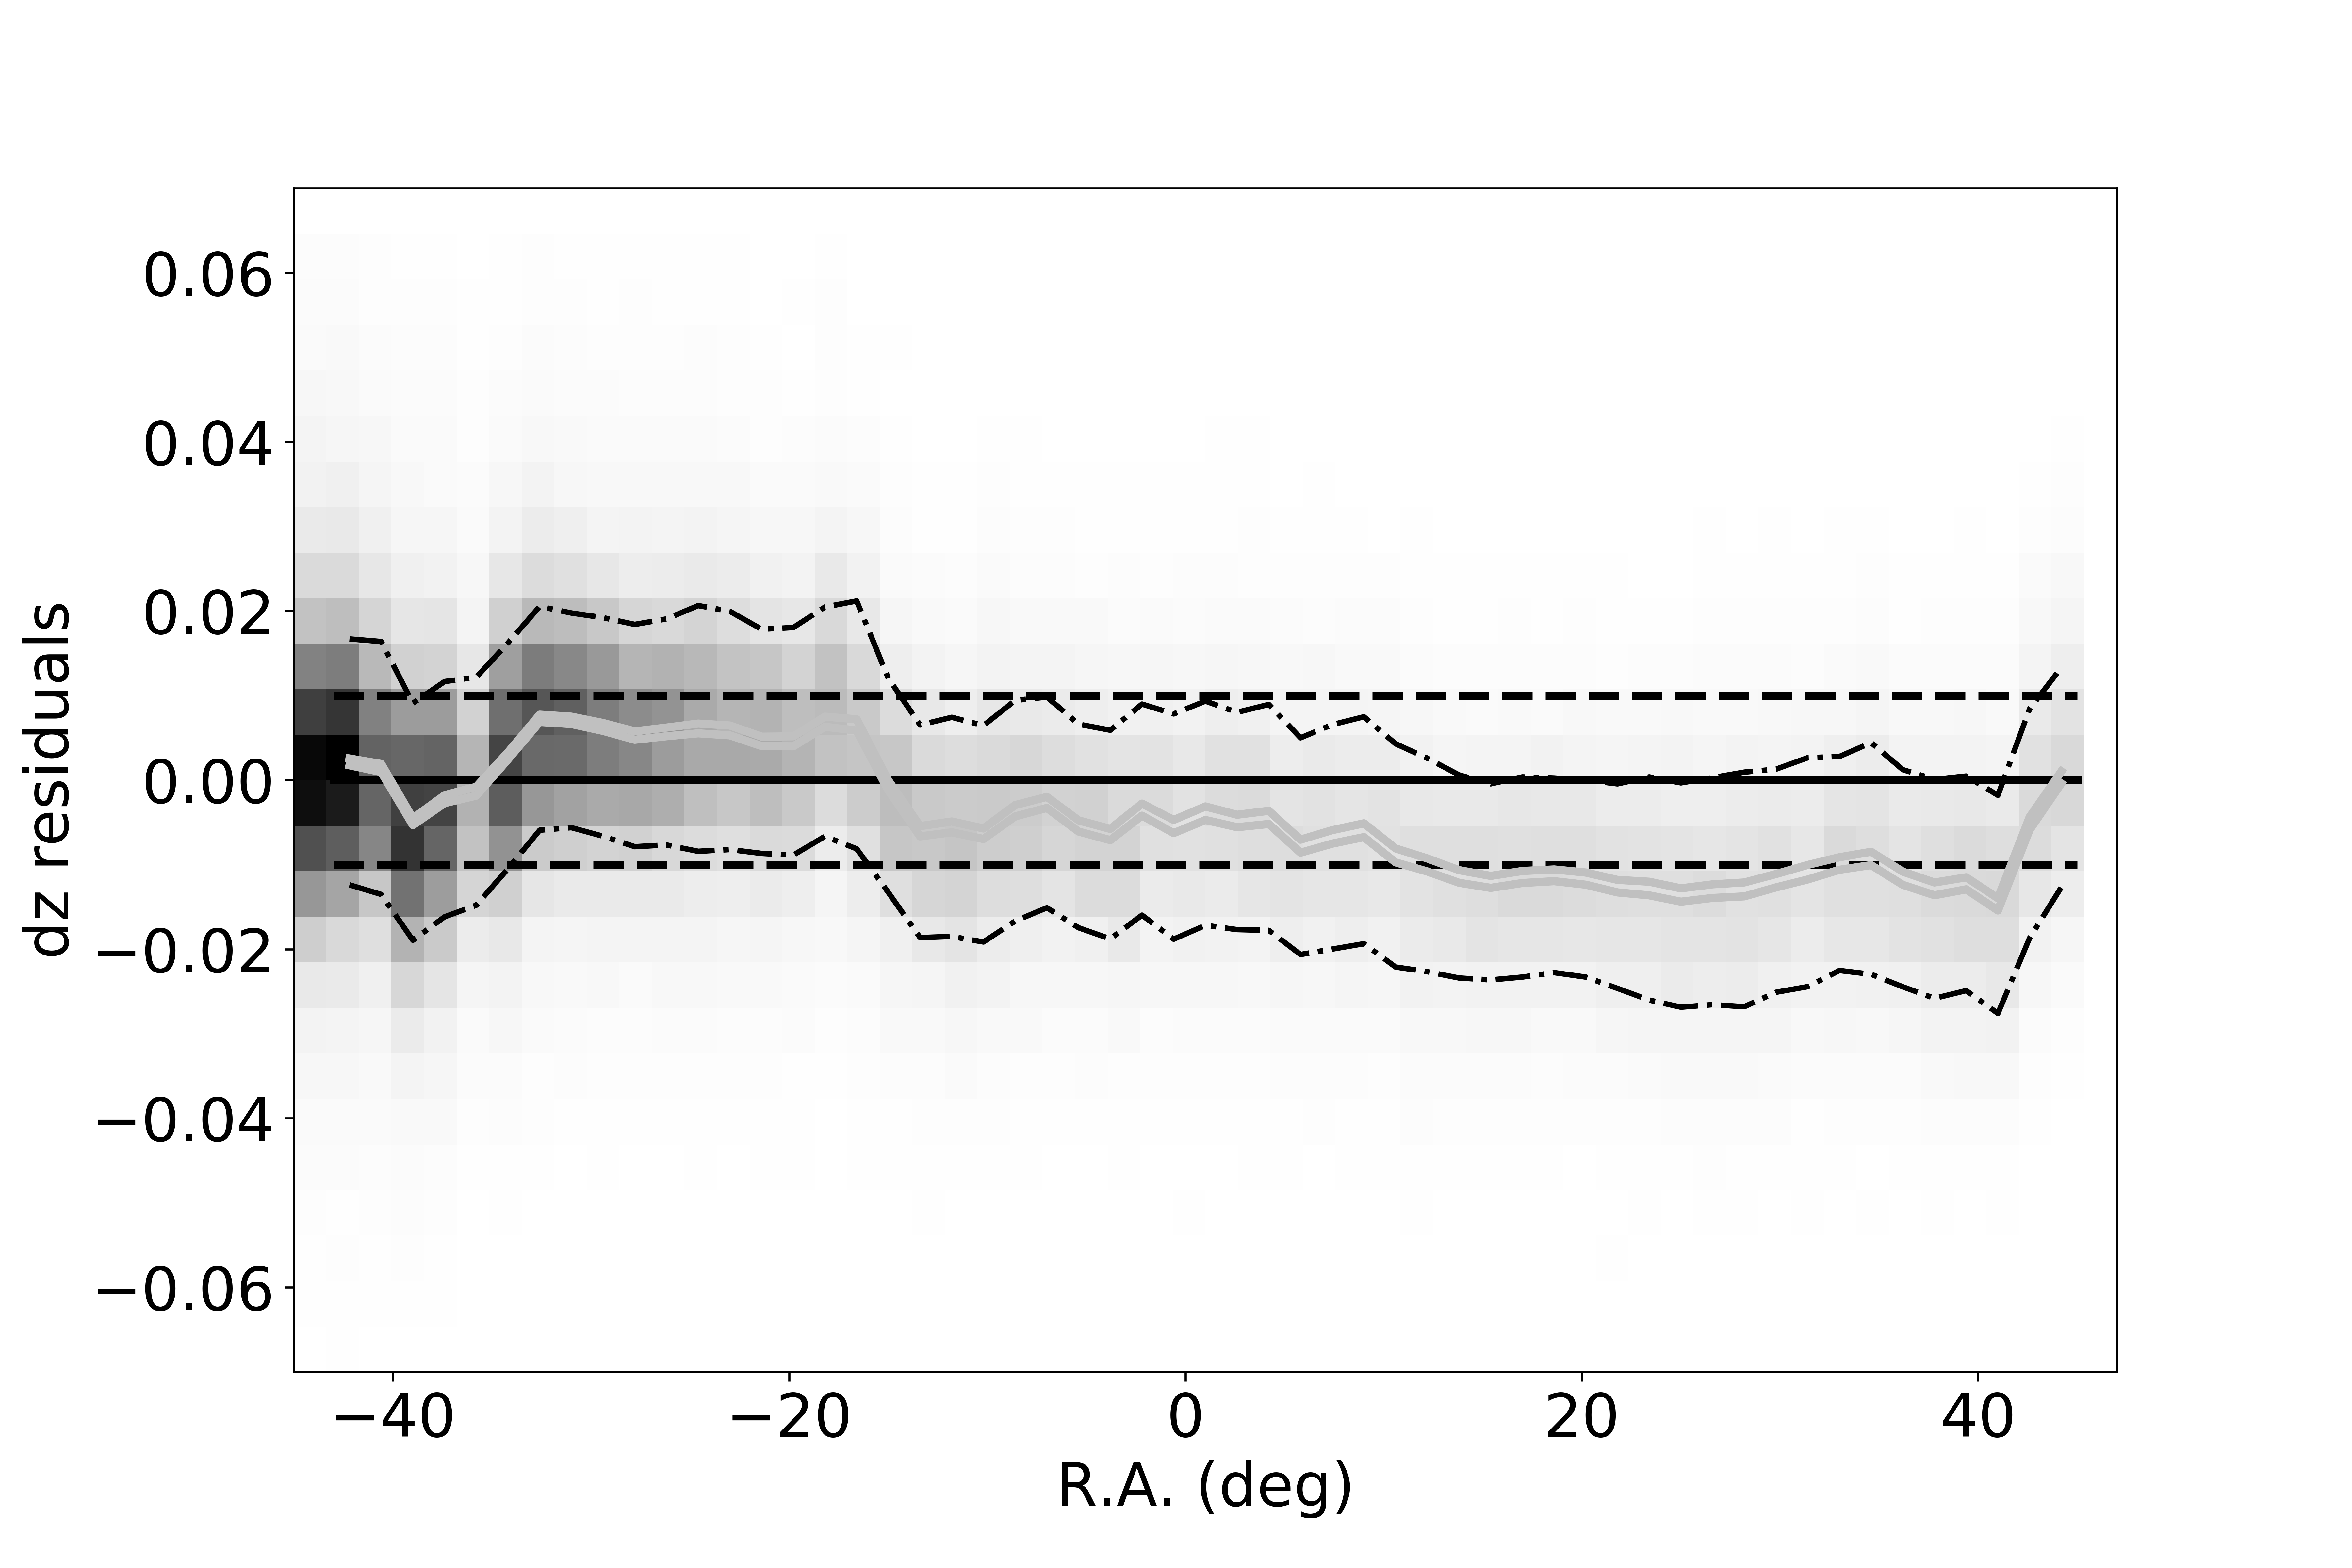
\includegraphics[width=7cm]{figures/colorResidPSbright_dz_RA_Hess.png}
\caption{A comparison of the magnitude differences between the SDSS v3.4 catalog
and DES (left) and Pan-STARRS (right) catalogs, for the $riz$ bands.}
\label{fig:DESPSRA}
\end{figure}

\begin{figure}[th!]
    \centering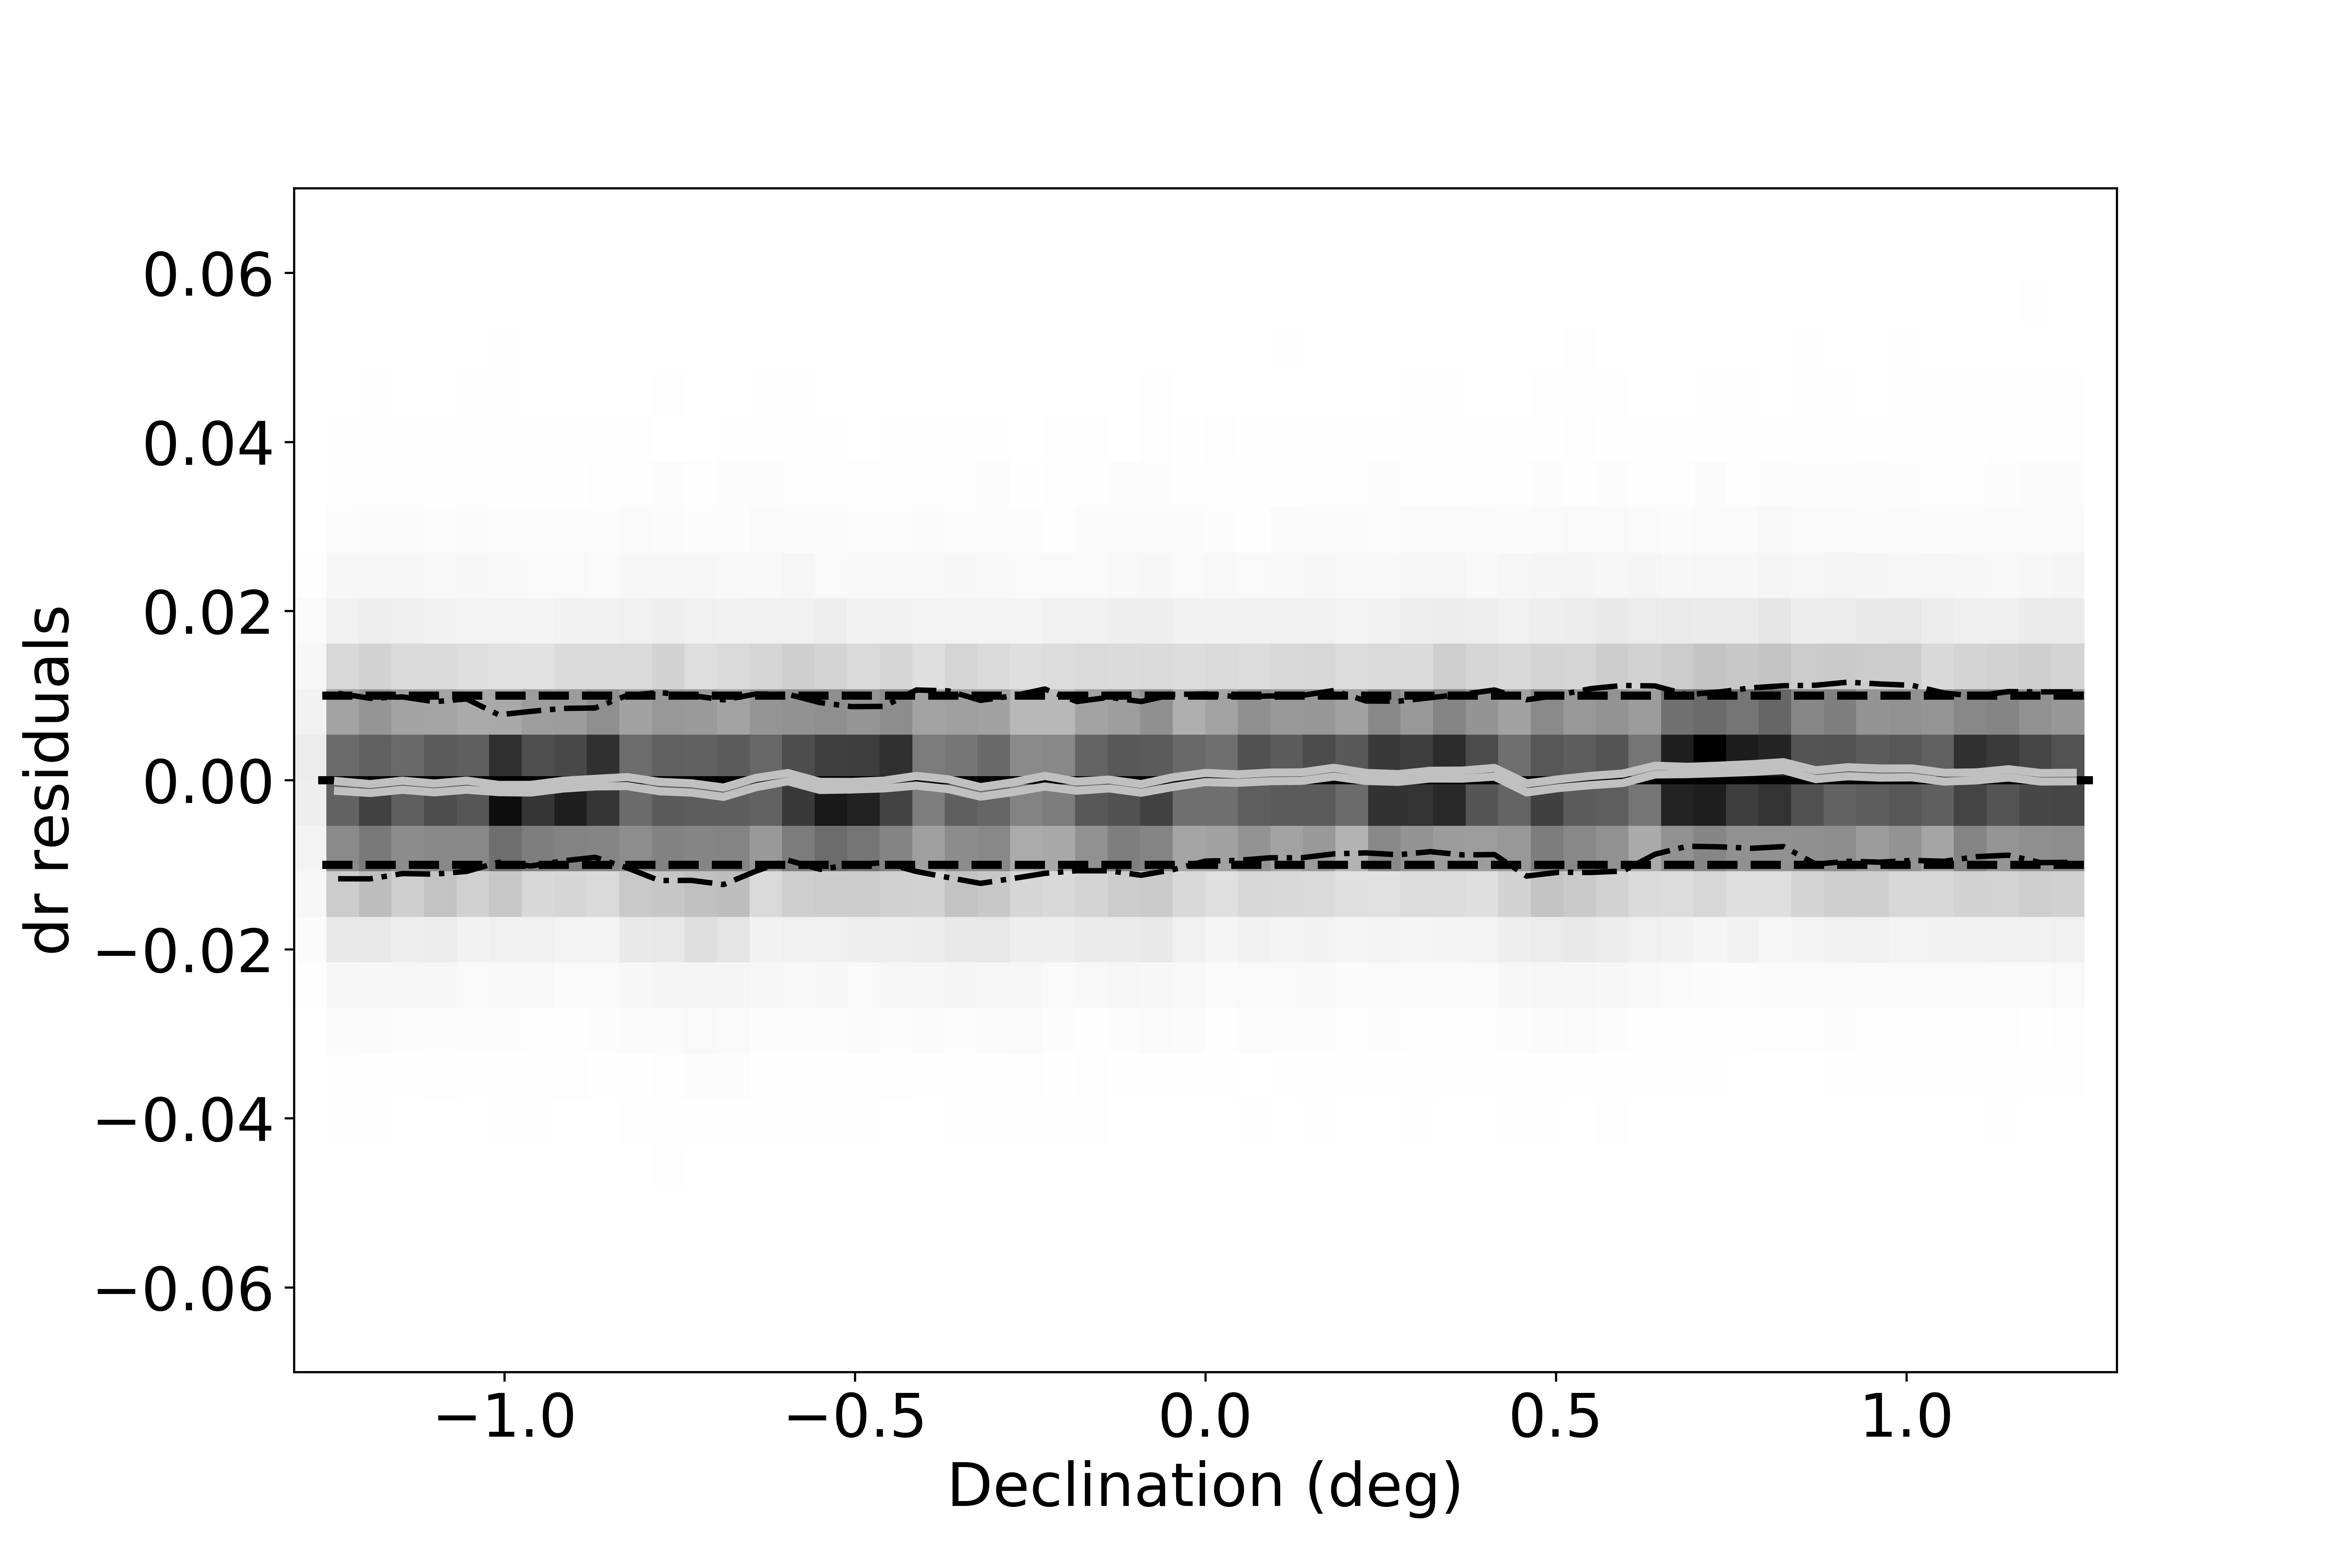
\includegraphics[width=7cm]{figures/colorResidDES2bright_dr_Dec_Hess.png}
    \centering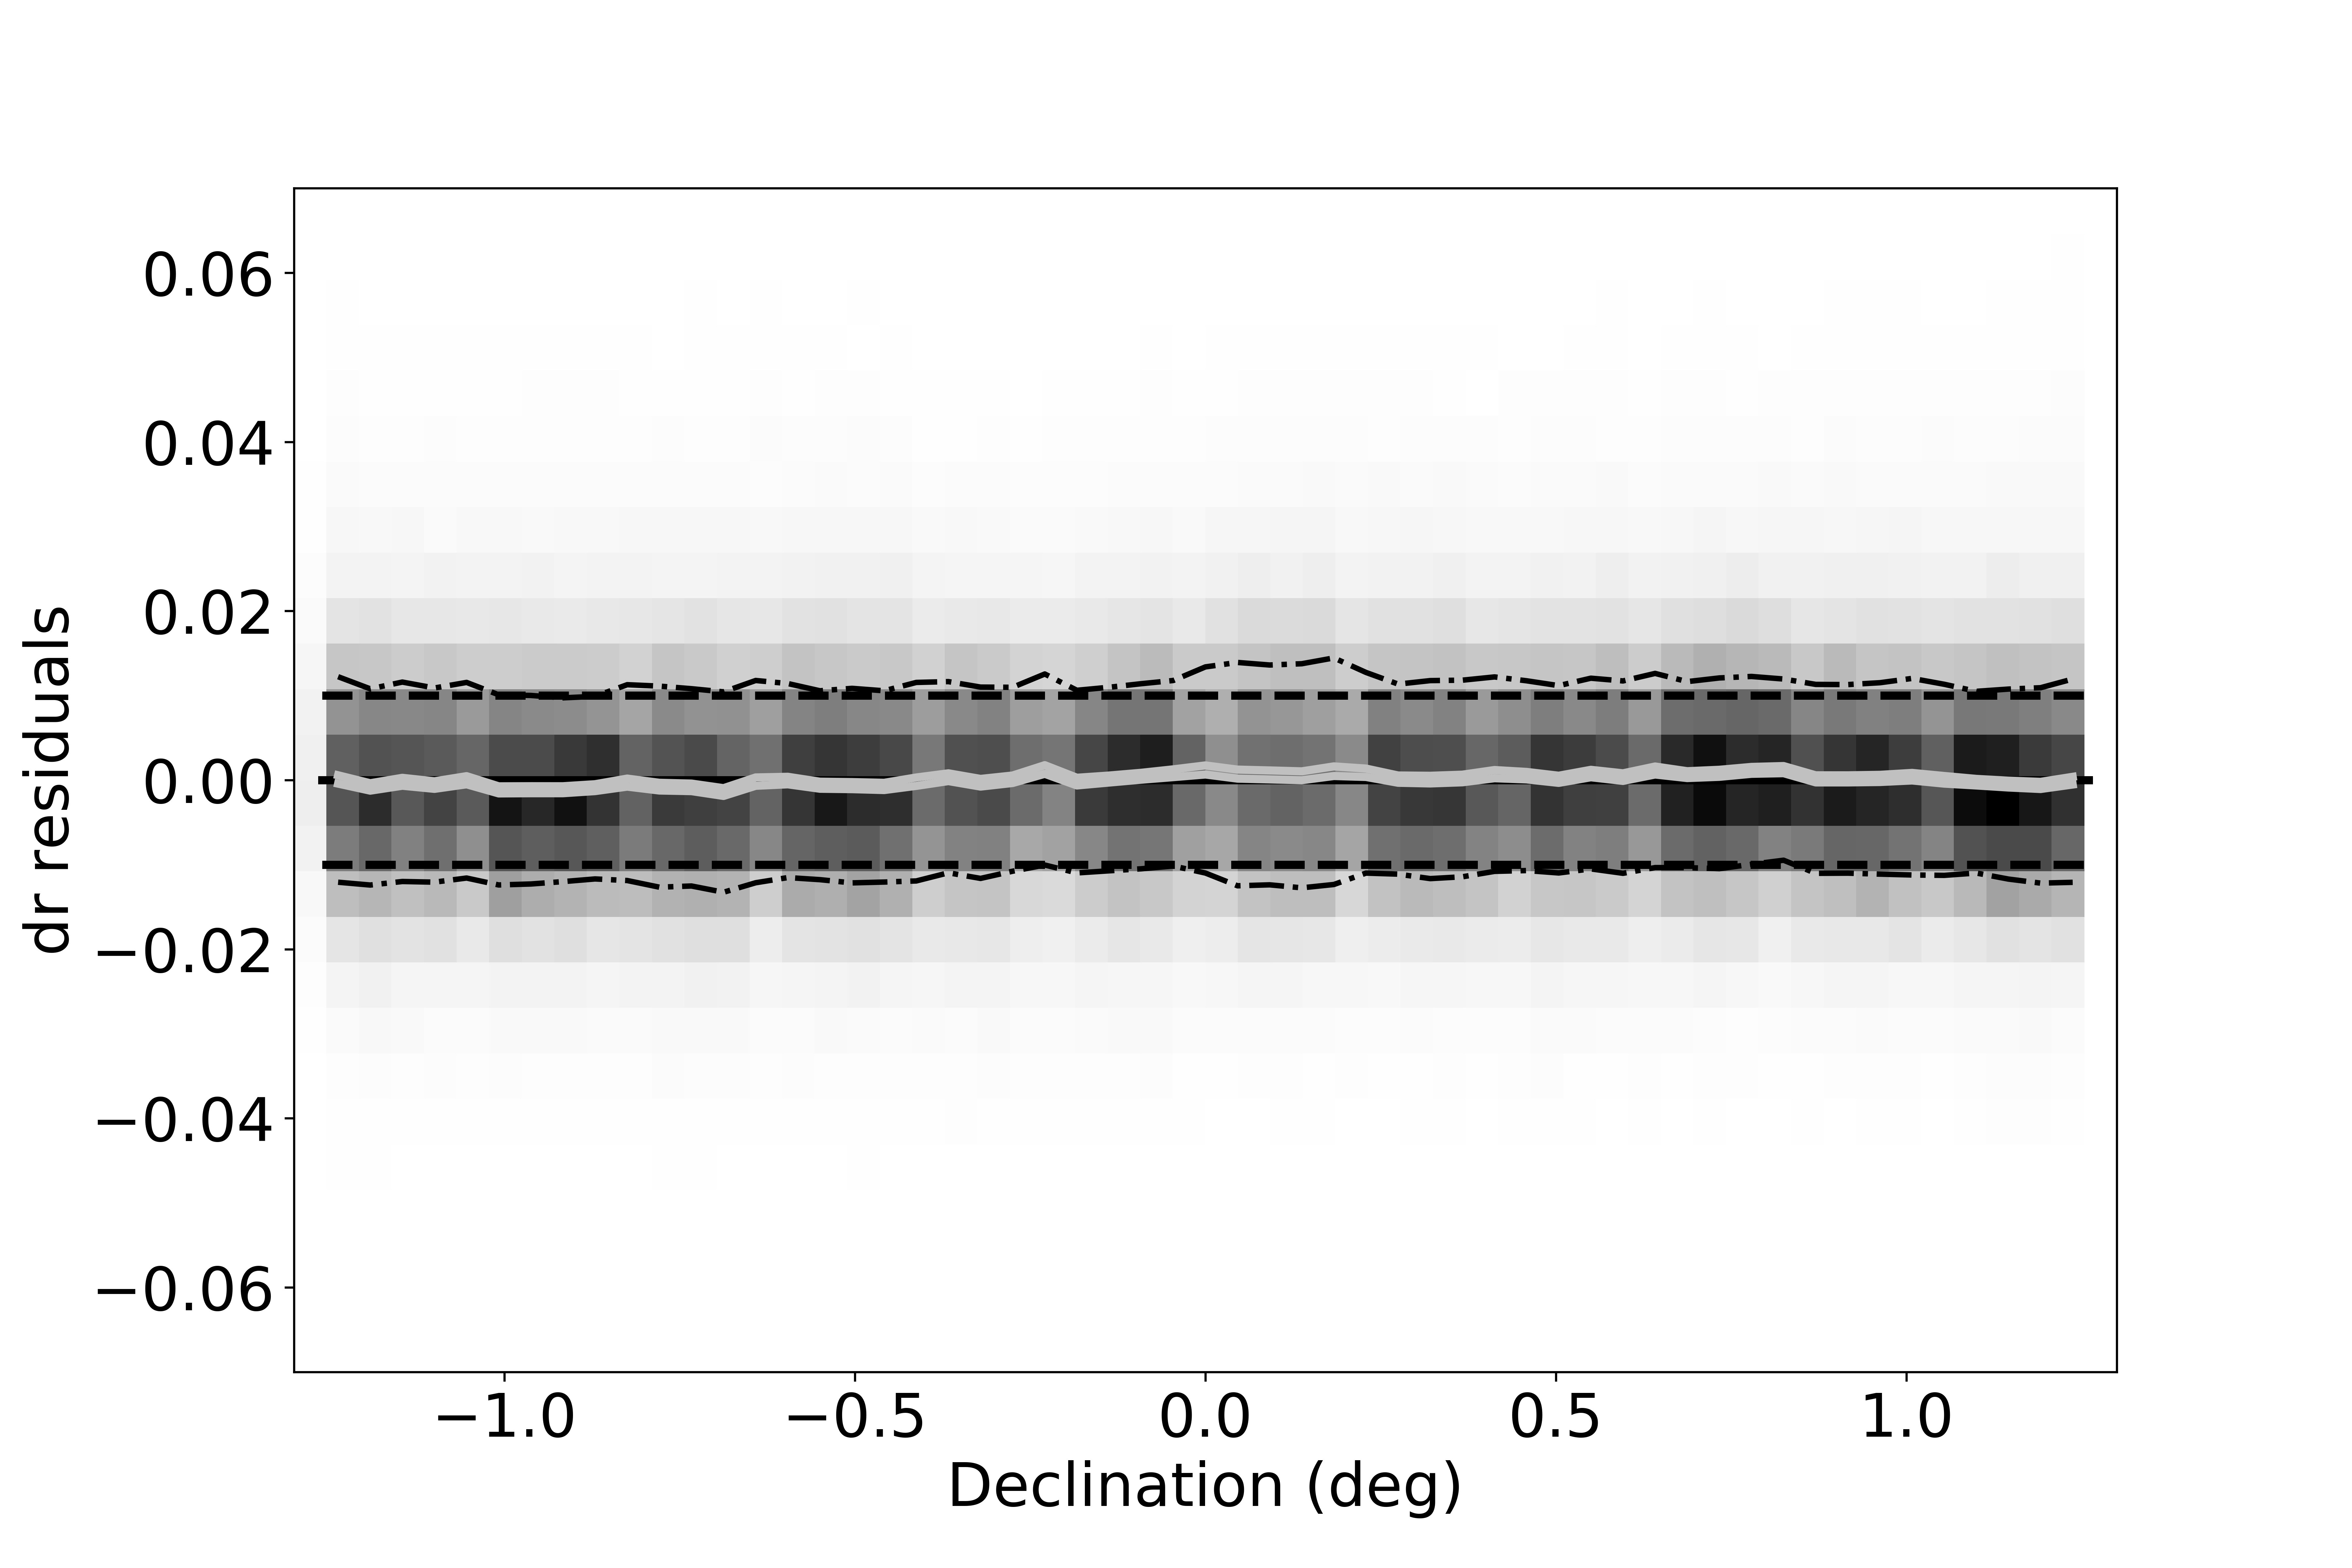
\includegraphics[width=7cm]{figures/colorResidPSbright_dr_Dec_Hess.png}
    \centering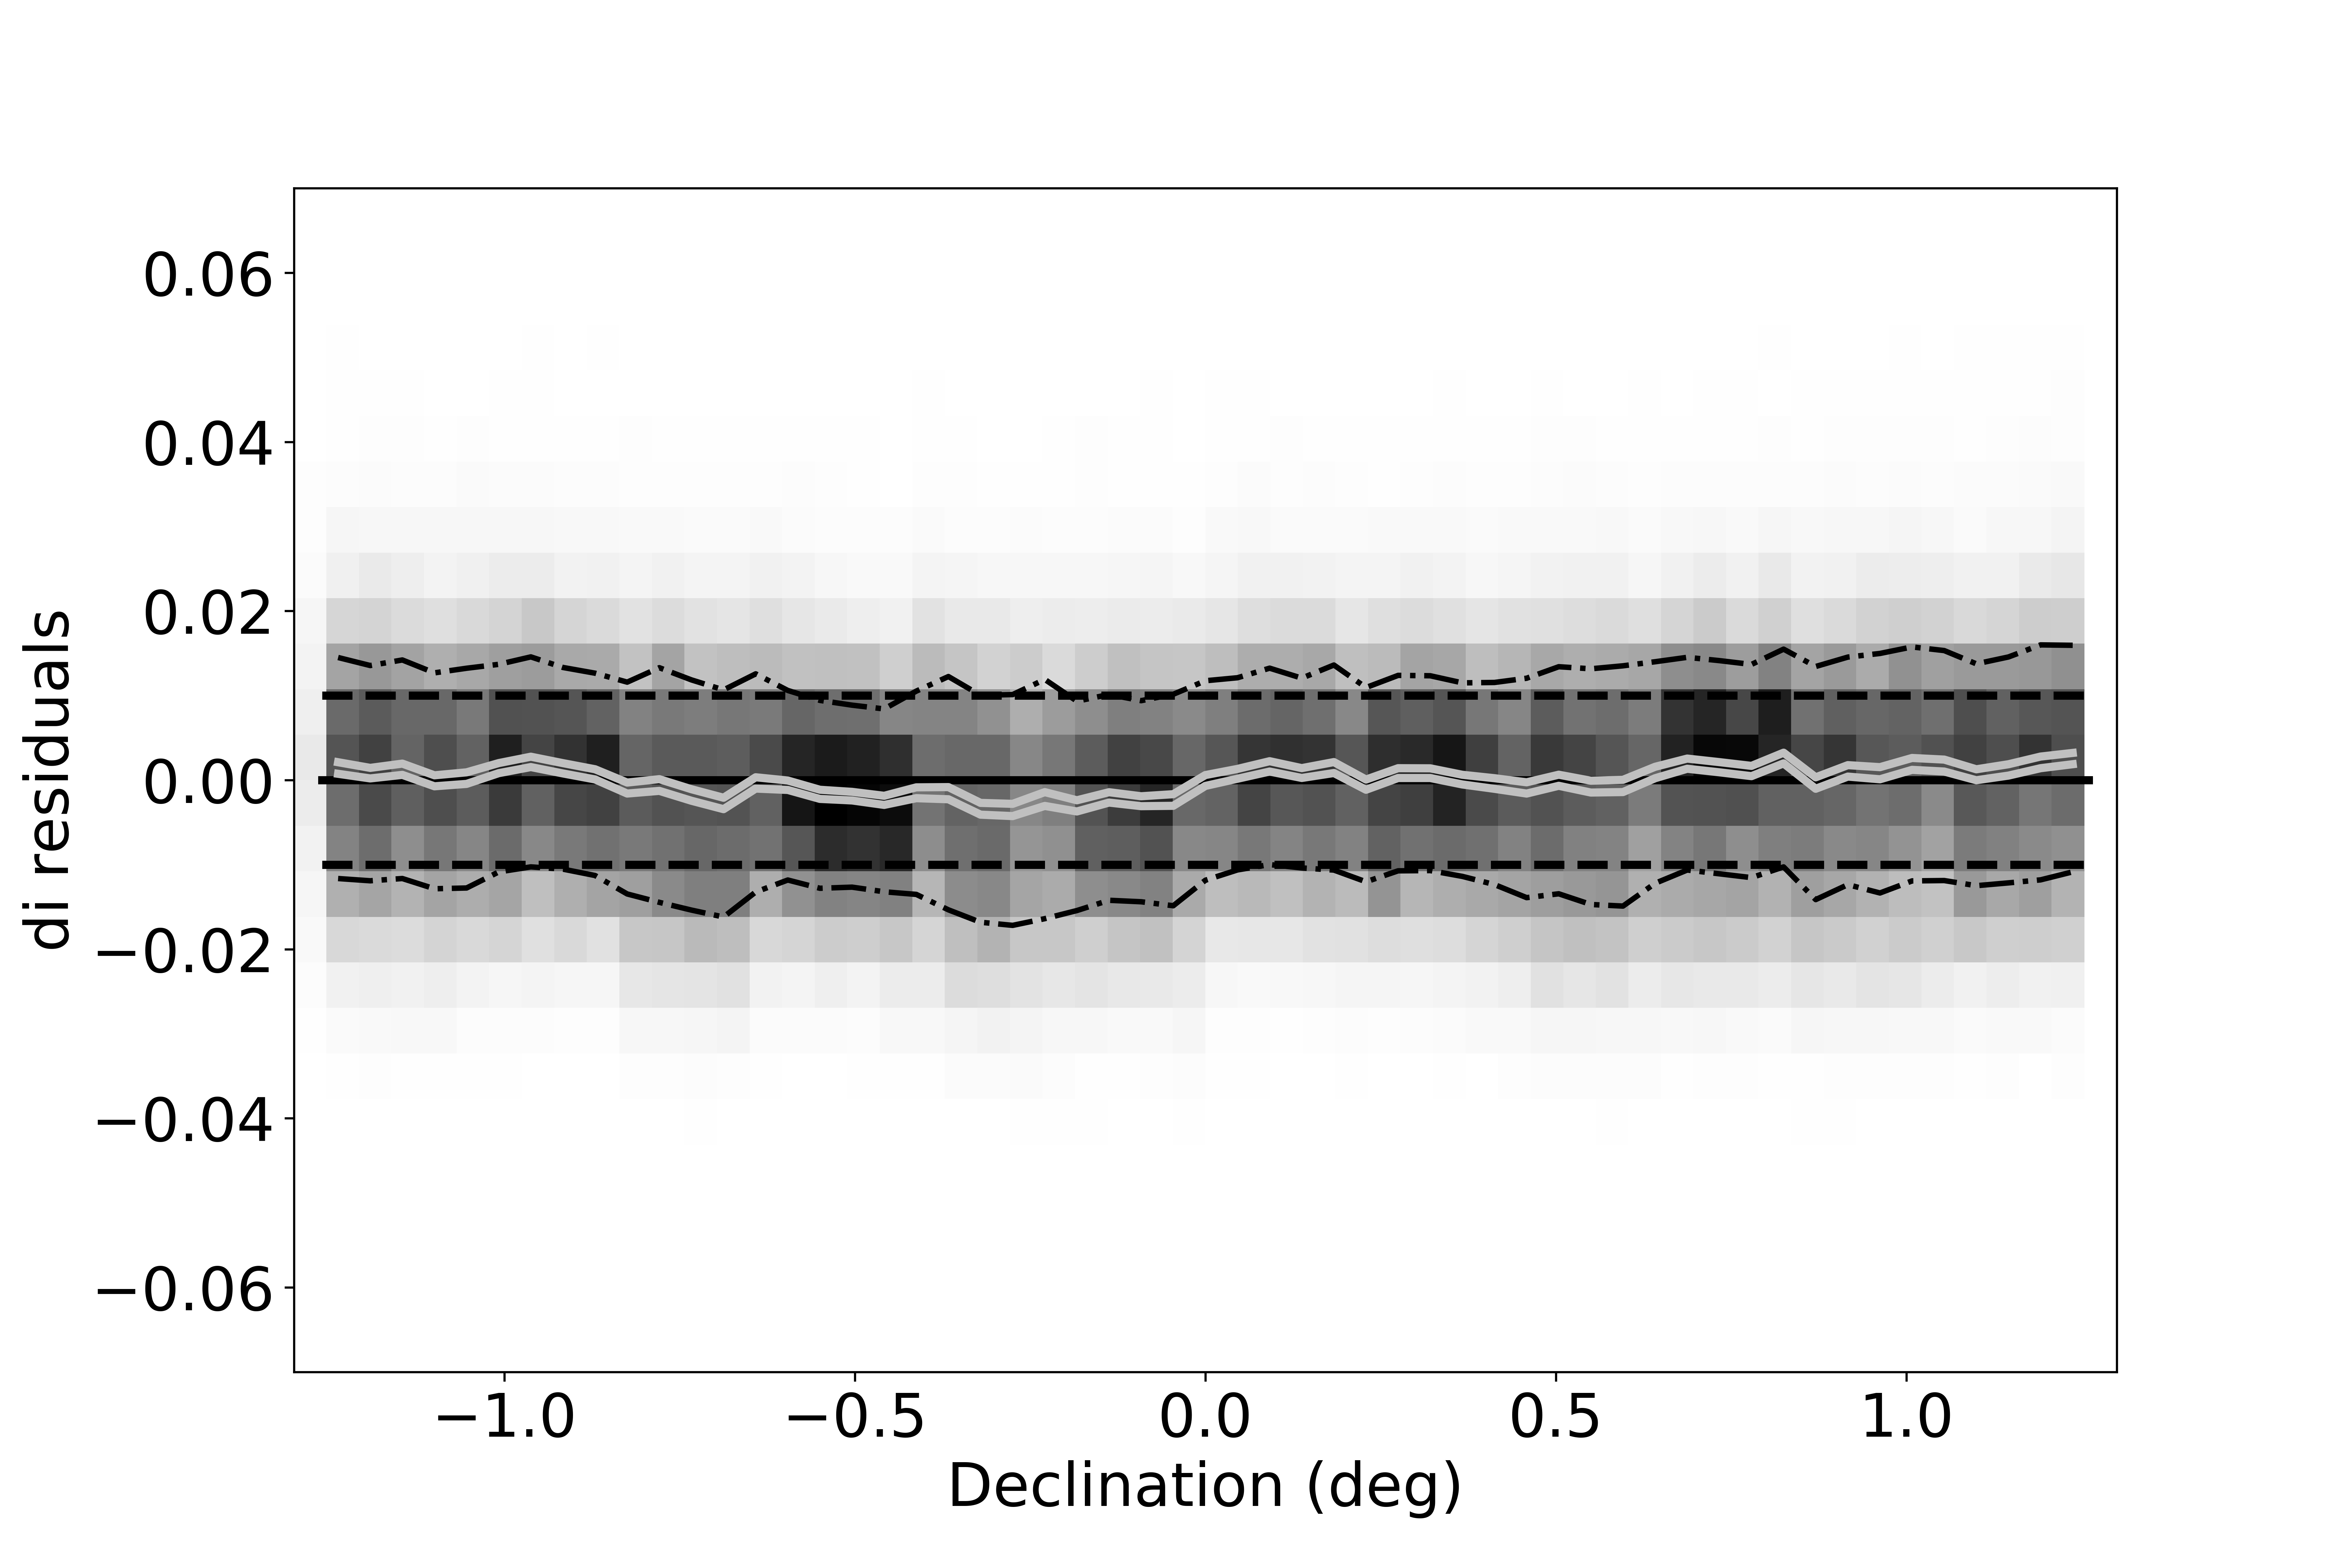
\includegraphics[width=7cm]{figures/colorResidDES2bright_di_Dec_Hess.png}
    \centering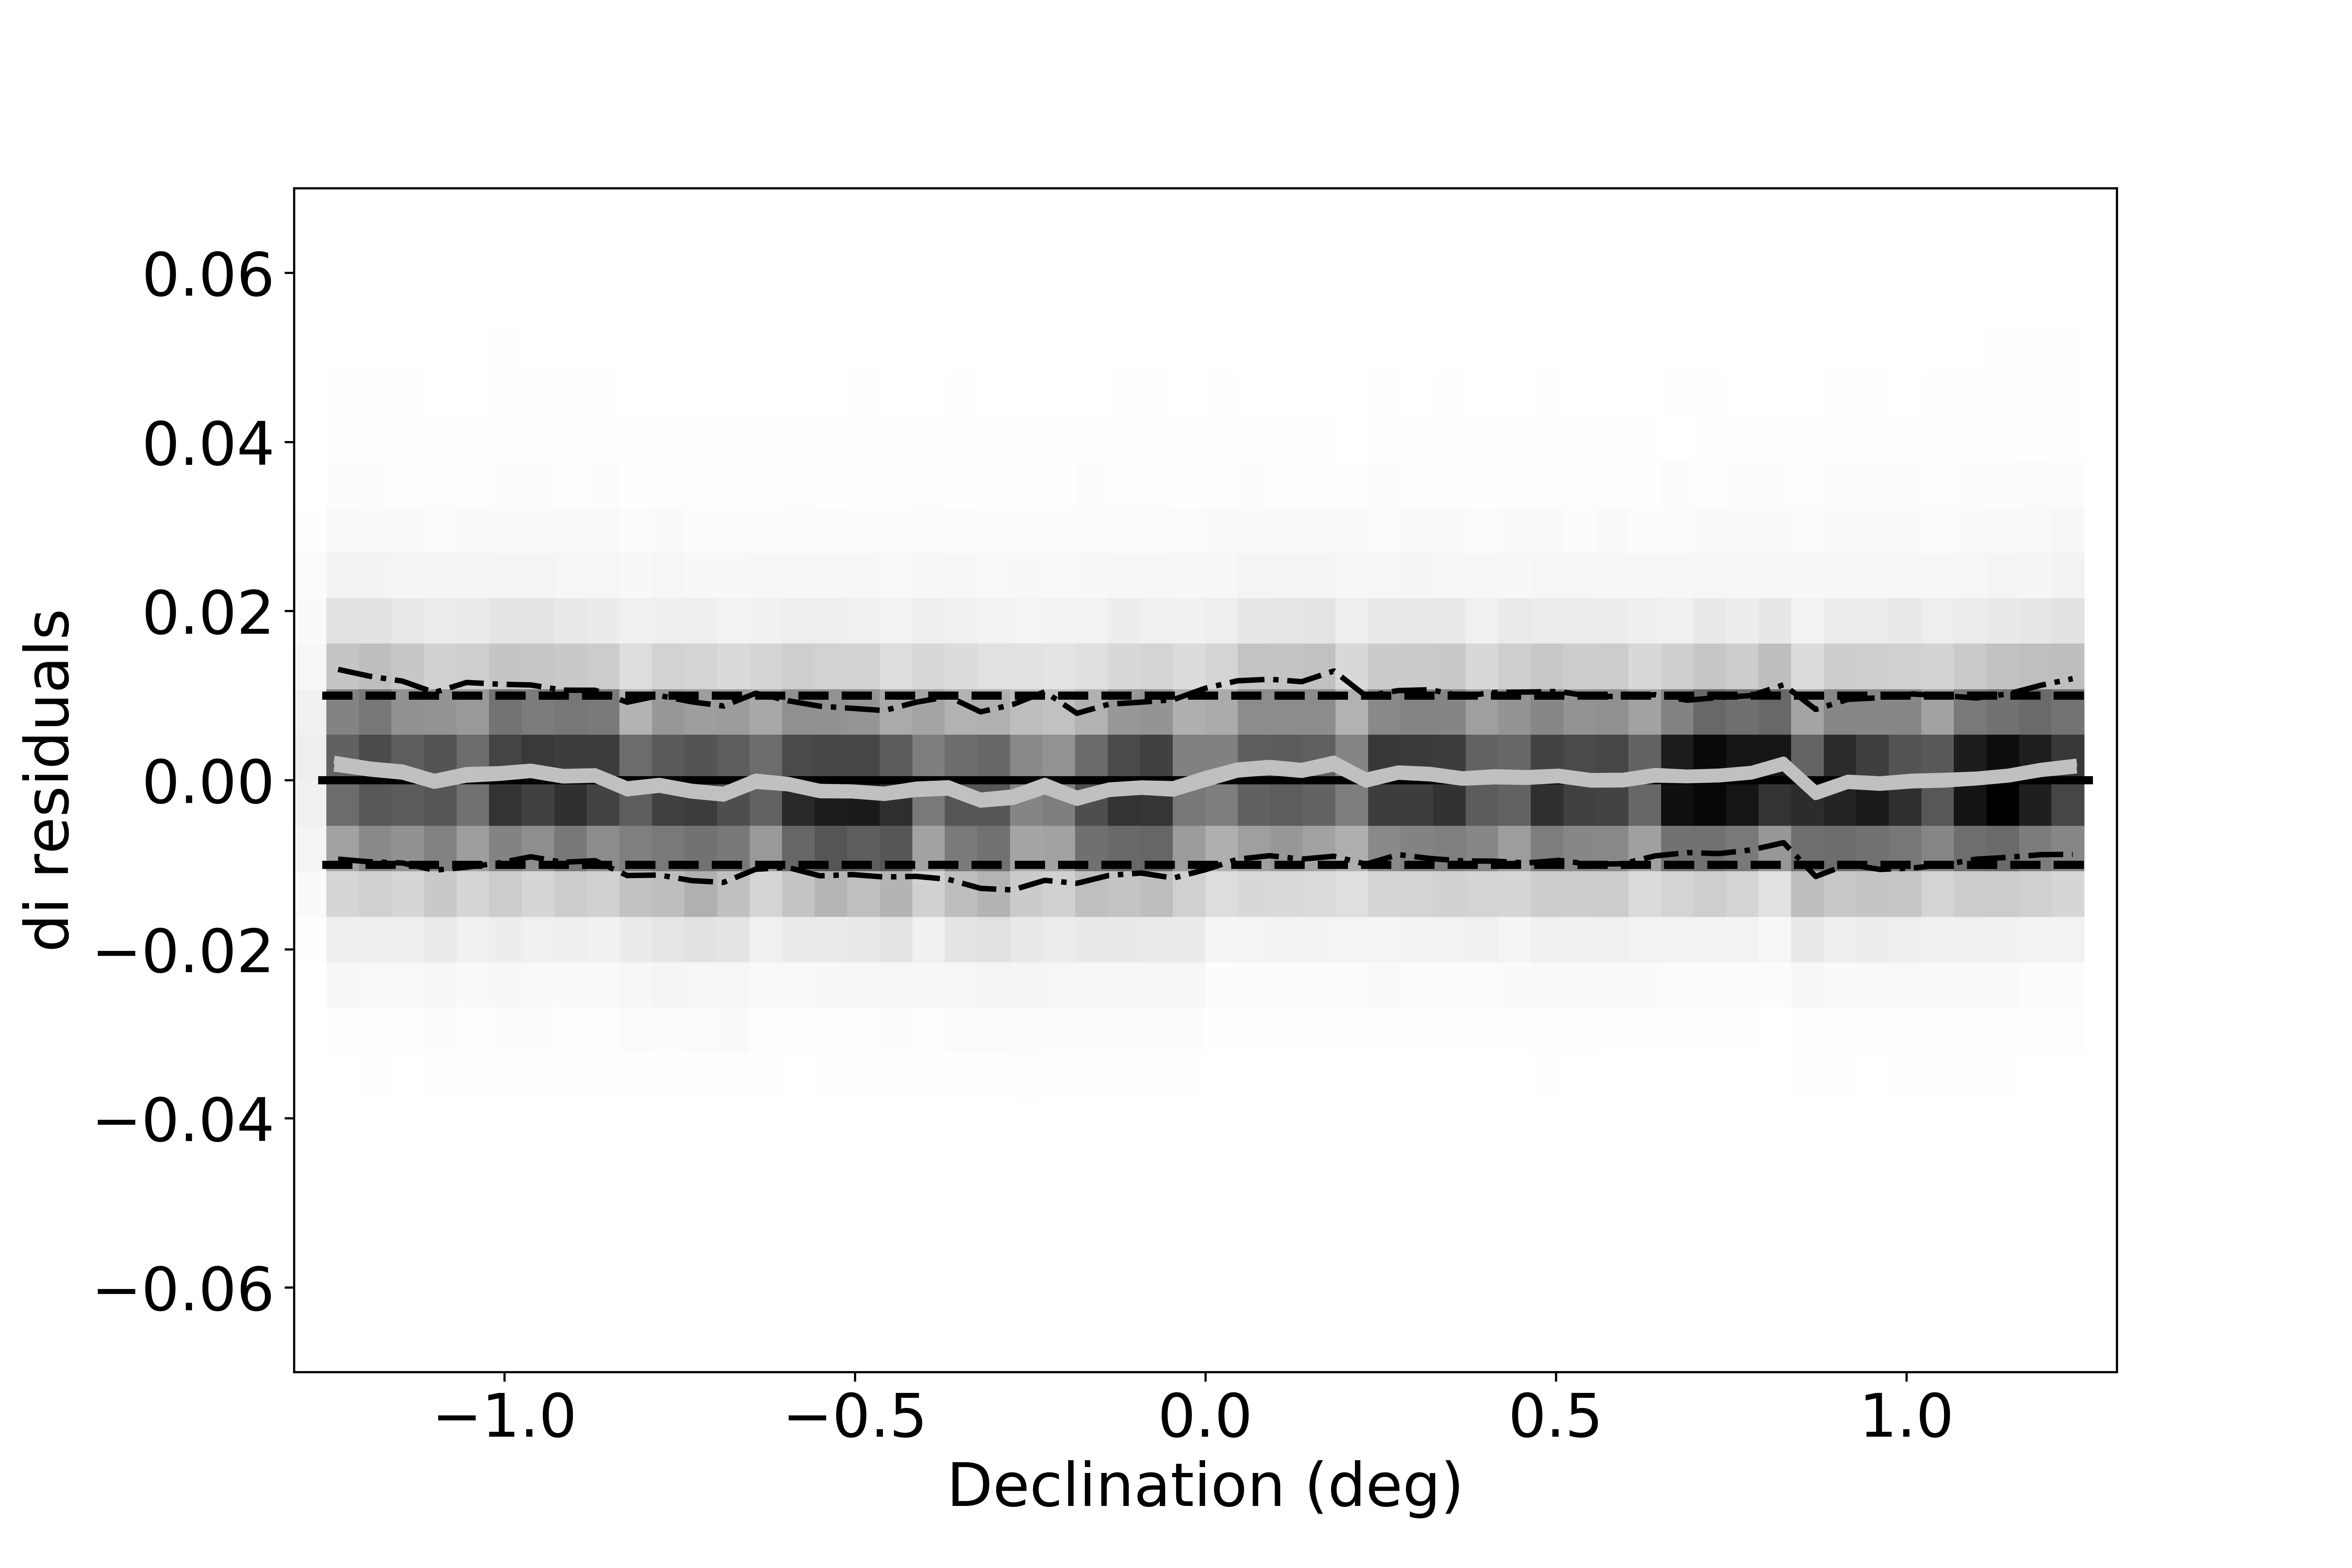
\includegraphics[width=7cm]{figures/colorResidPSbright_di_Dec_Hess.png}
    \centering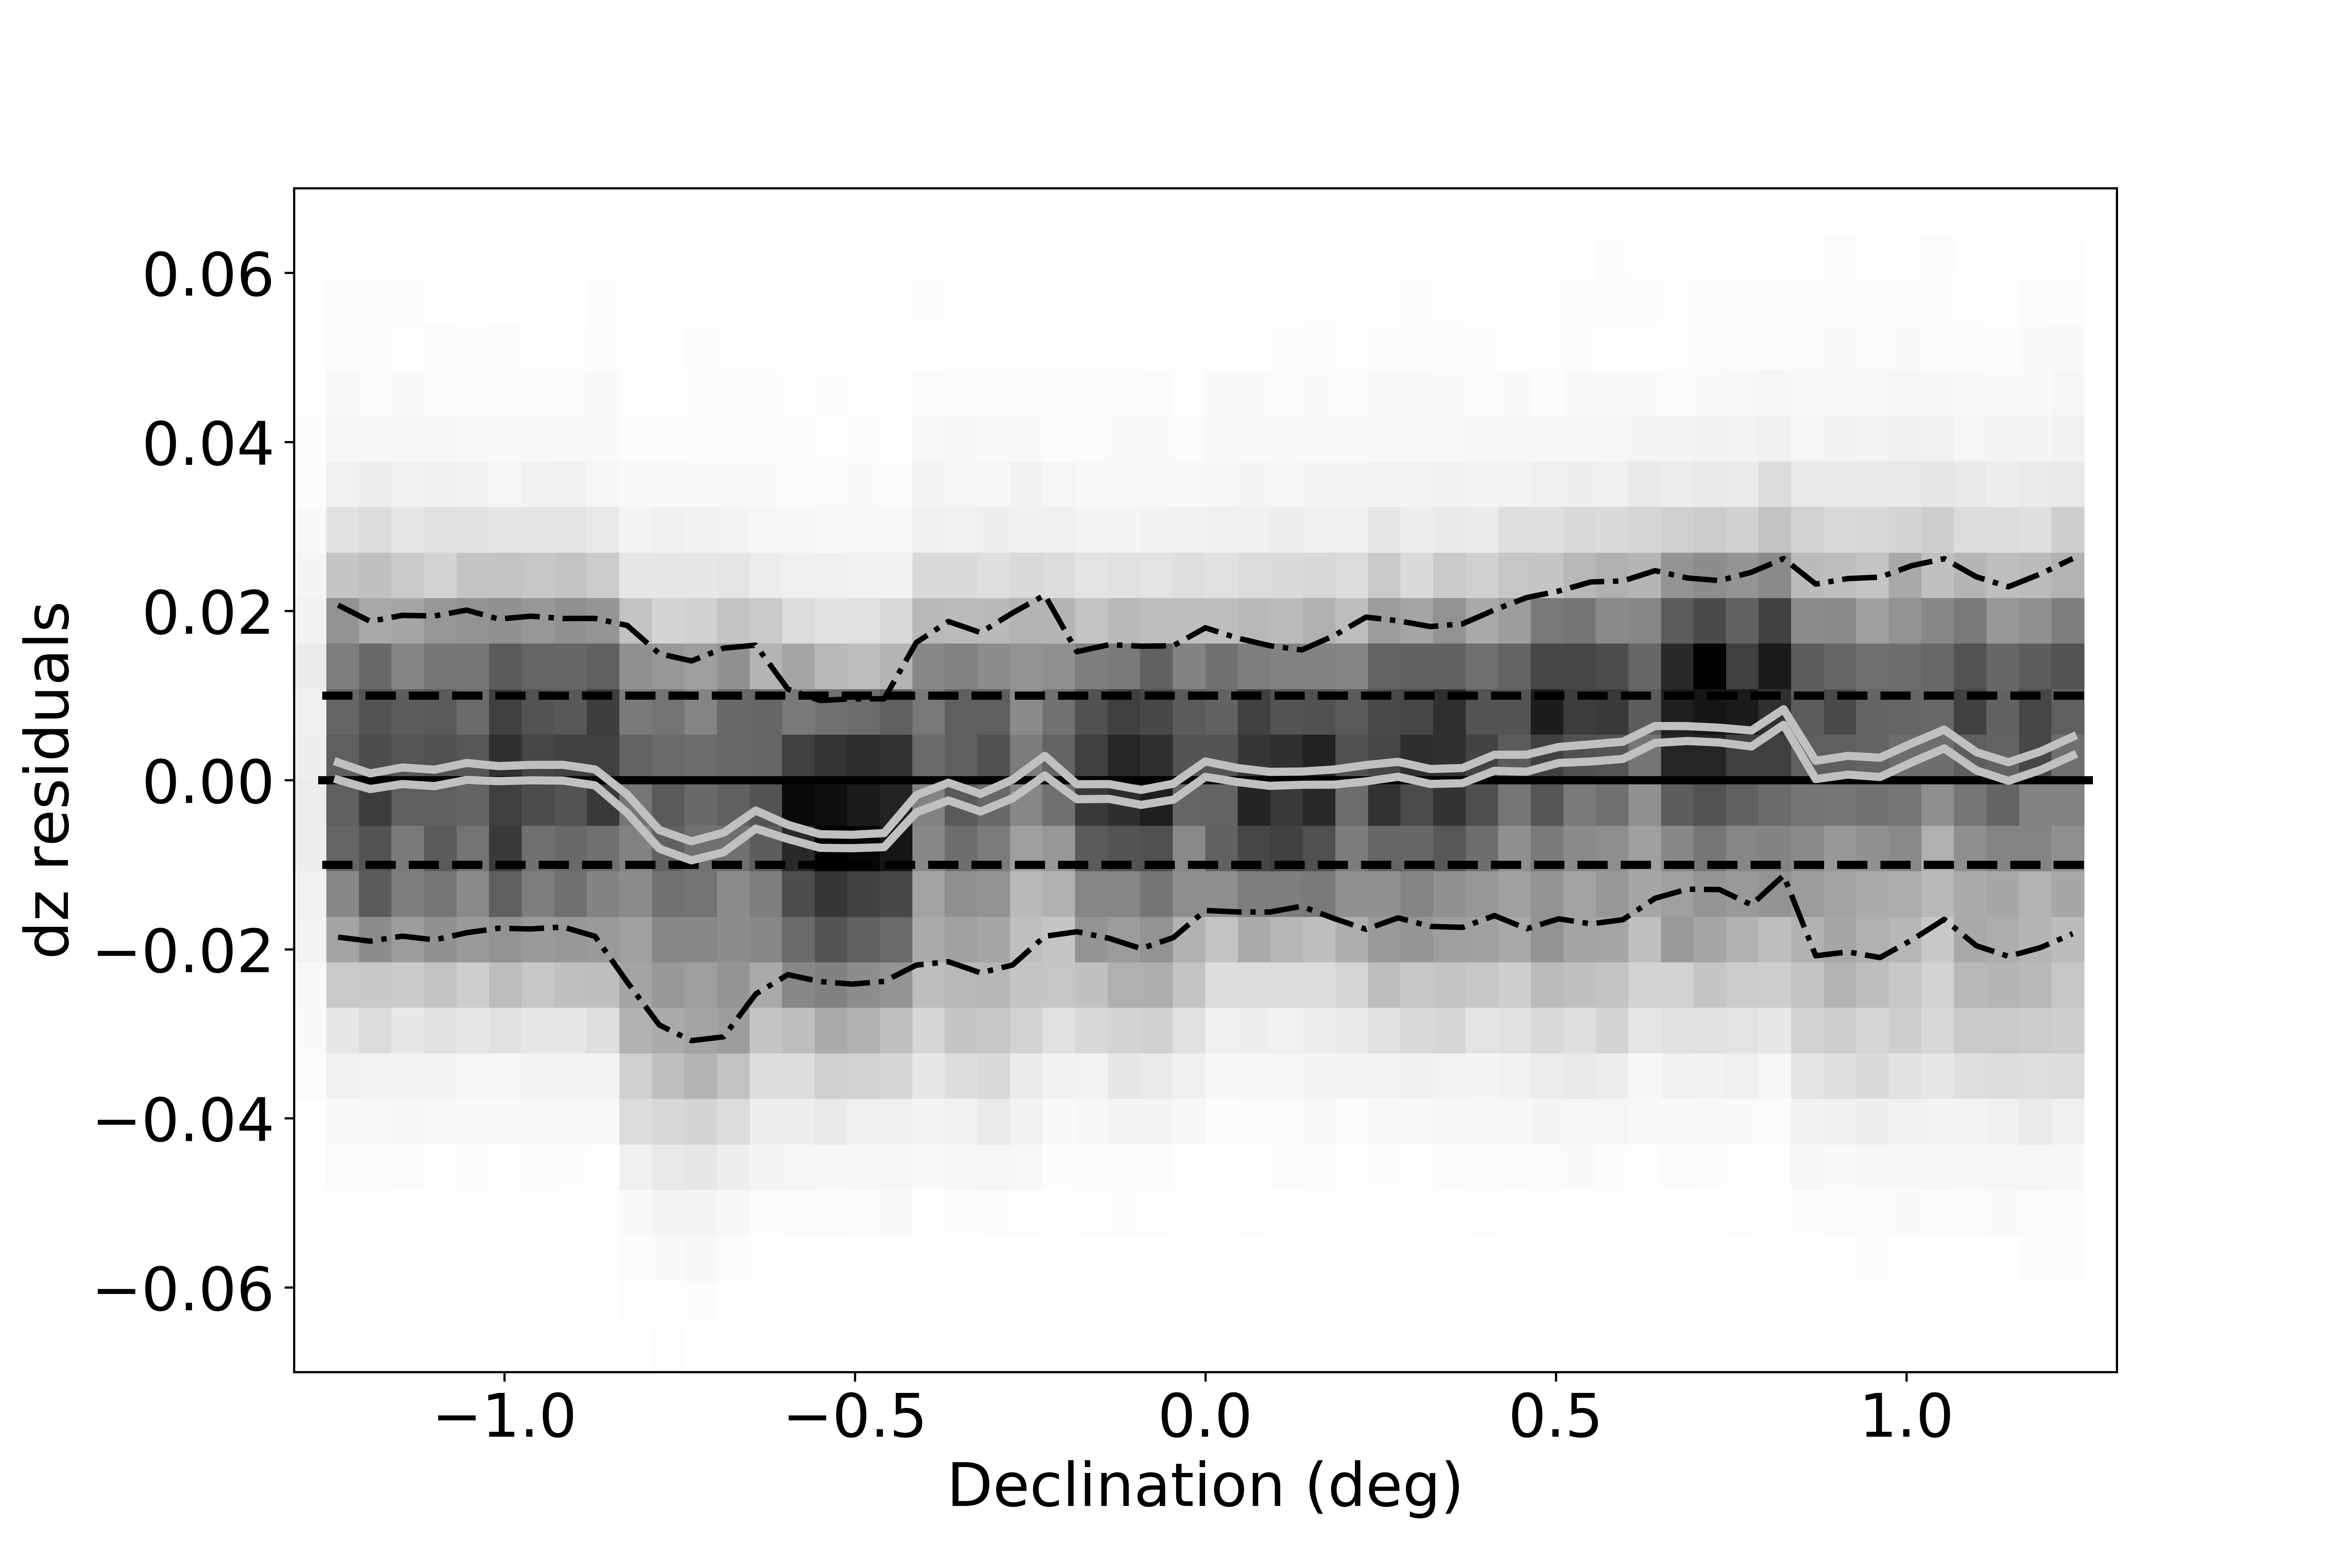
\includegraphics[width=7cm]{figures/colorResidDES2bright_dz_Dec_Hess.png}
    \centering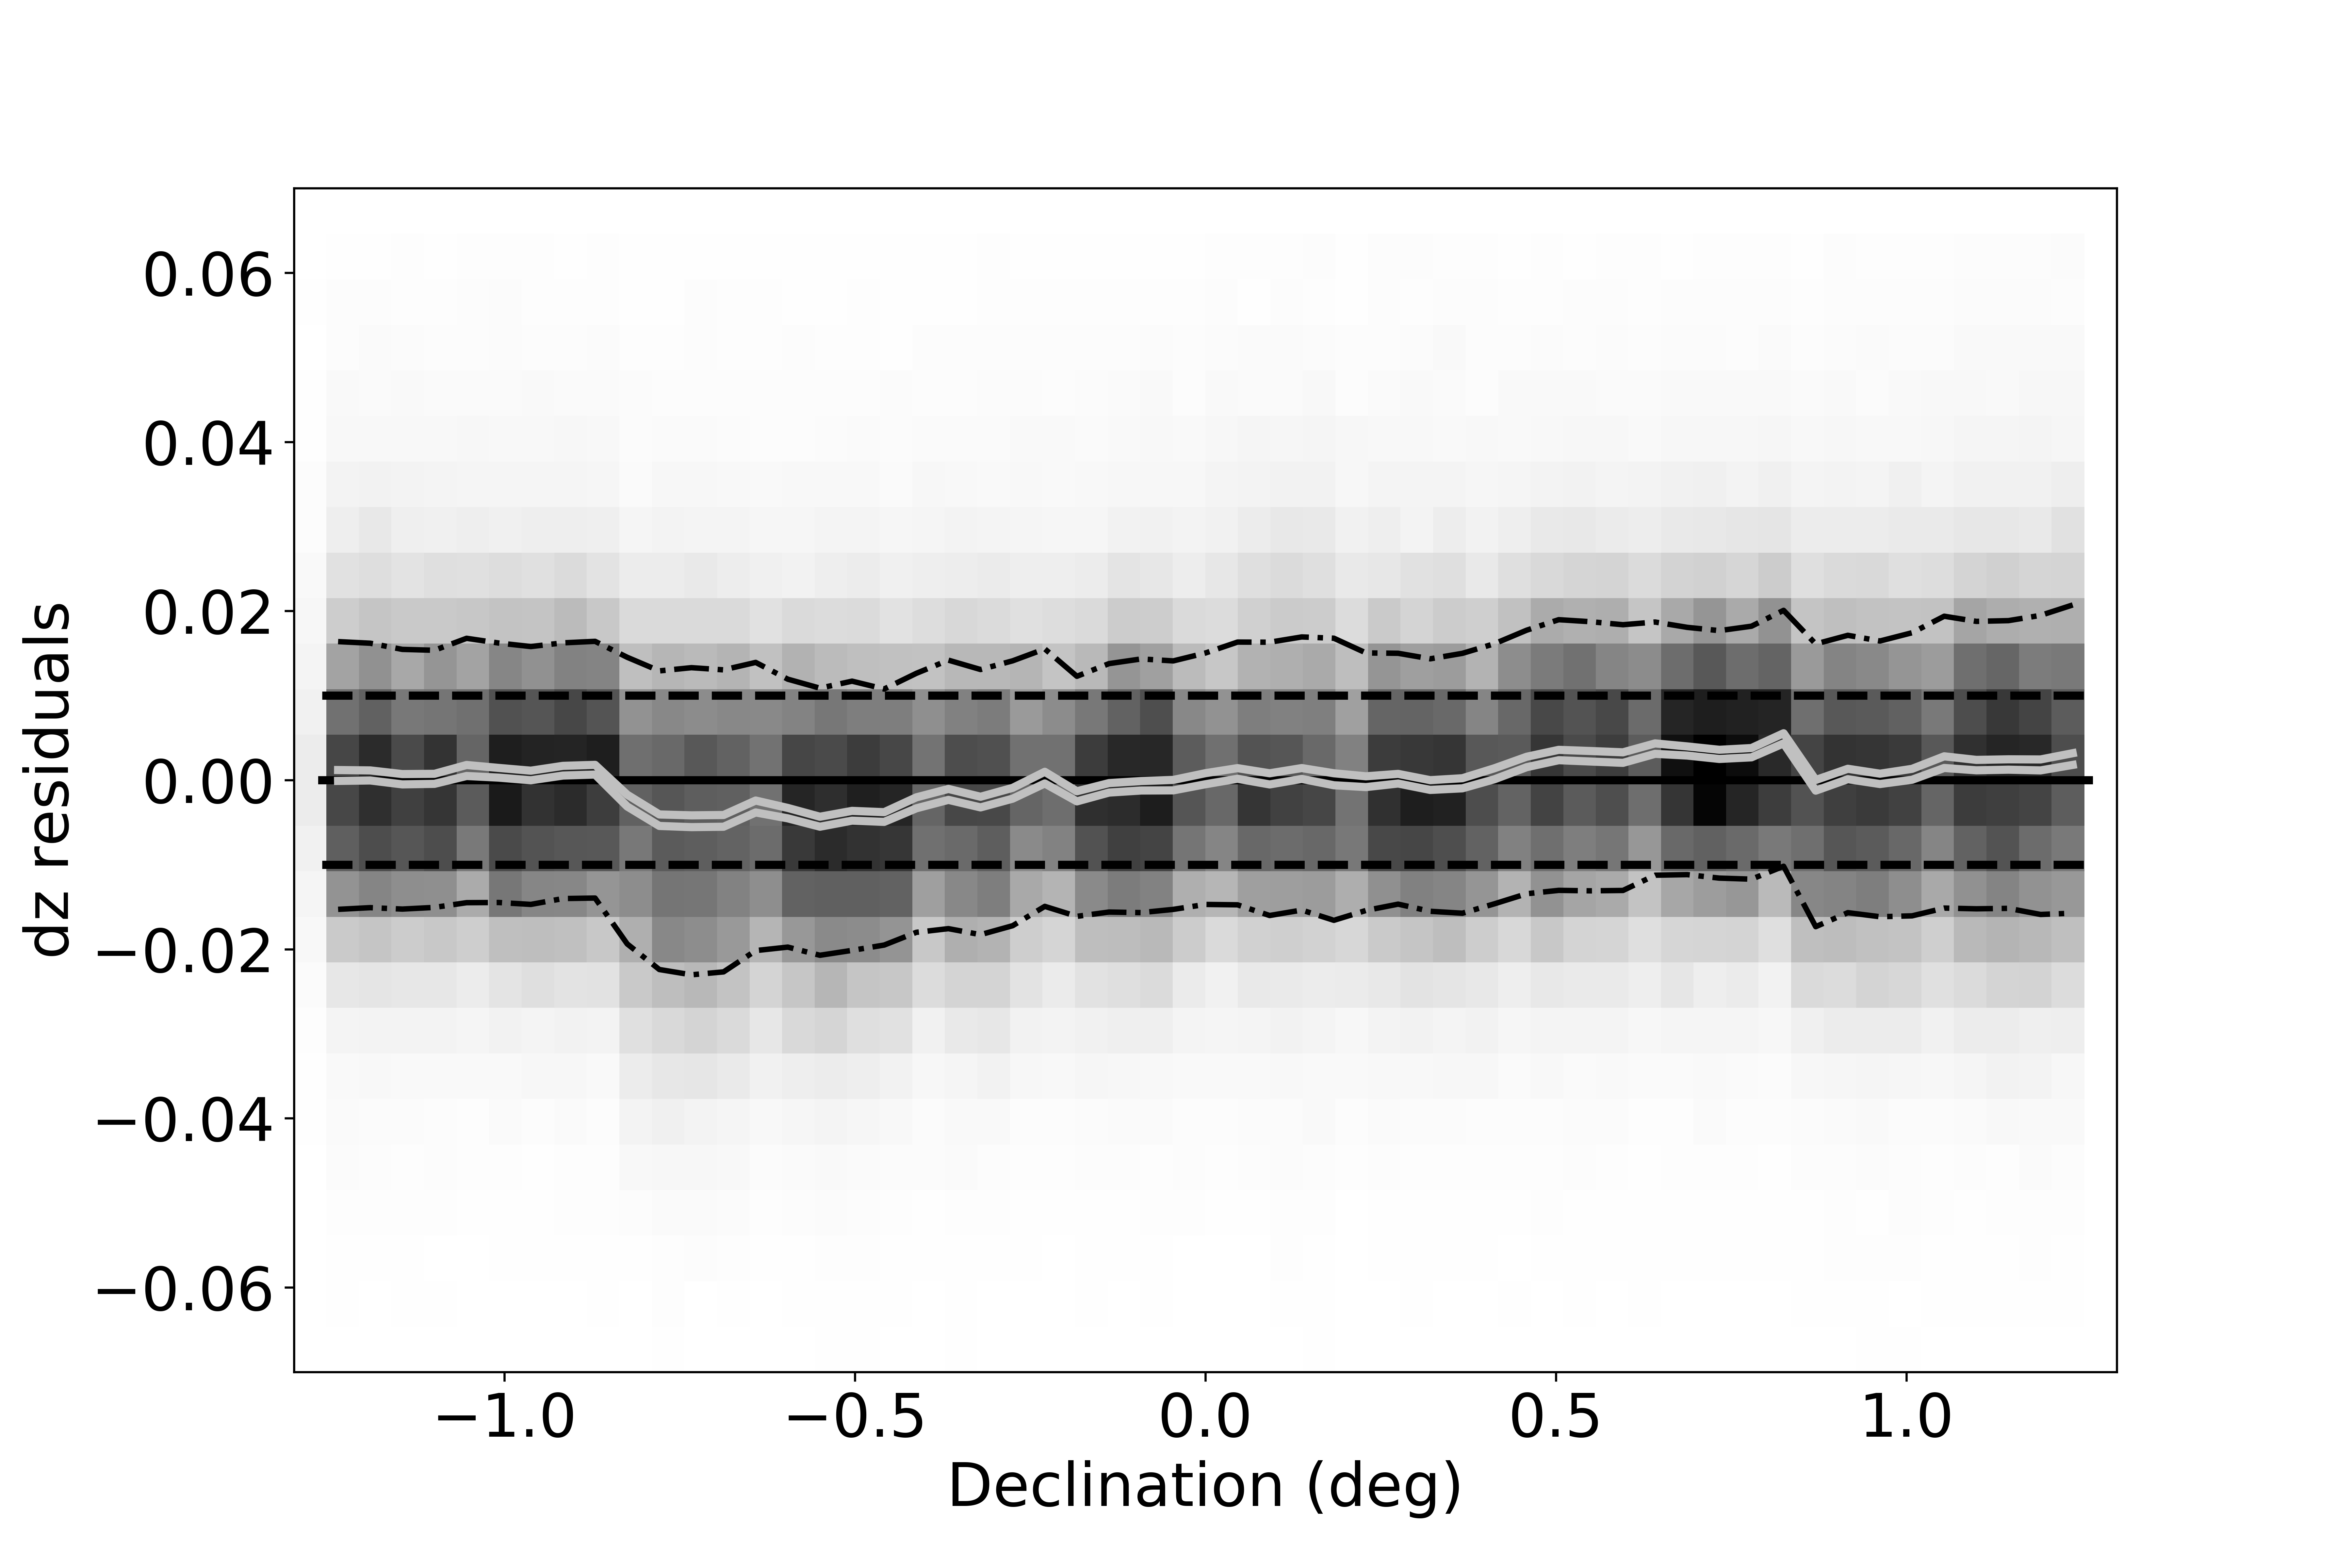
\includegraphics[width=7cm]{figures/colorResidPSbright_dz_Dec_Hess.png}
\caption{Analogous to Figure~\ref{fig:DESPSRA}, except that magnitude differences
are binned by Declination.}
\label{fig:DESPSDec}
\end{figure}

\begin{figure}[th!]
    \centering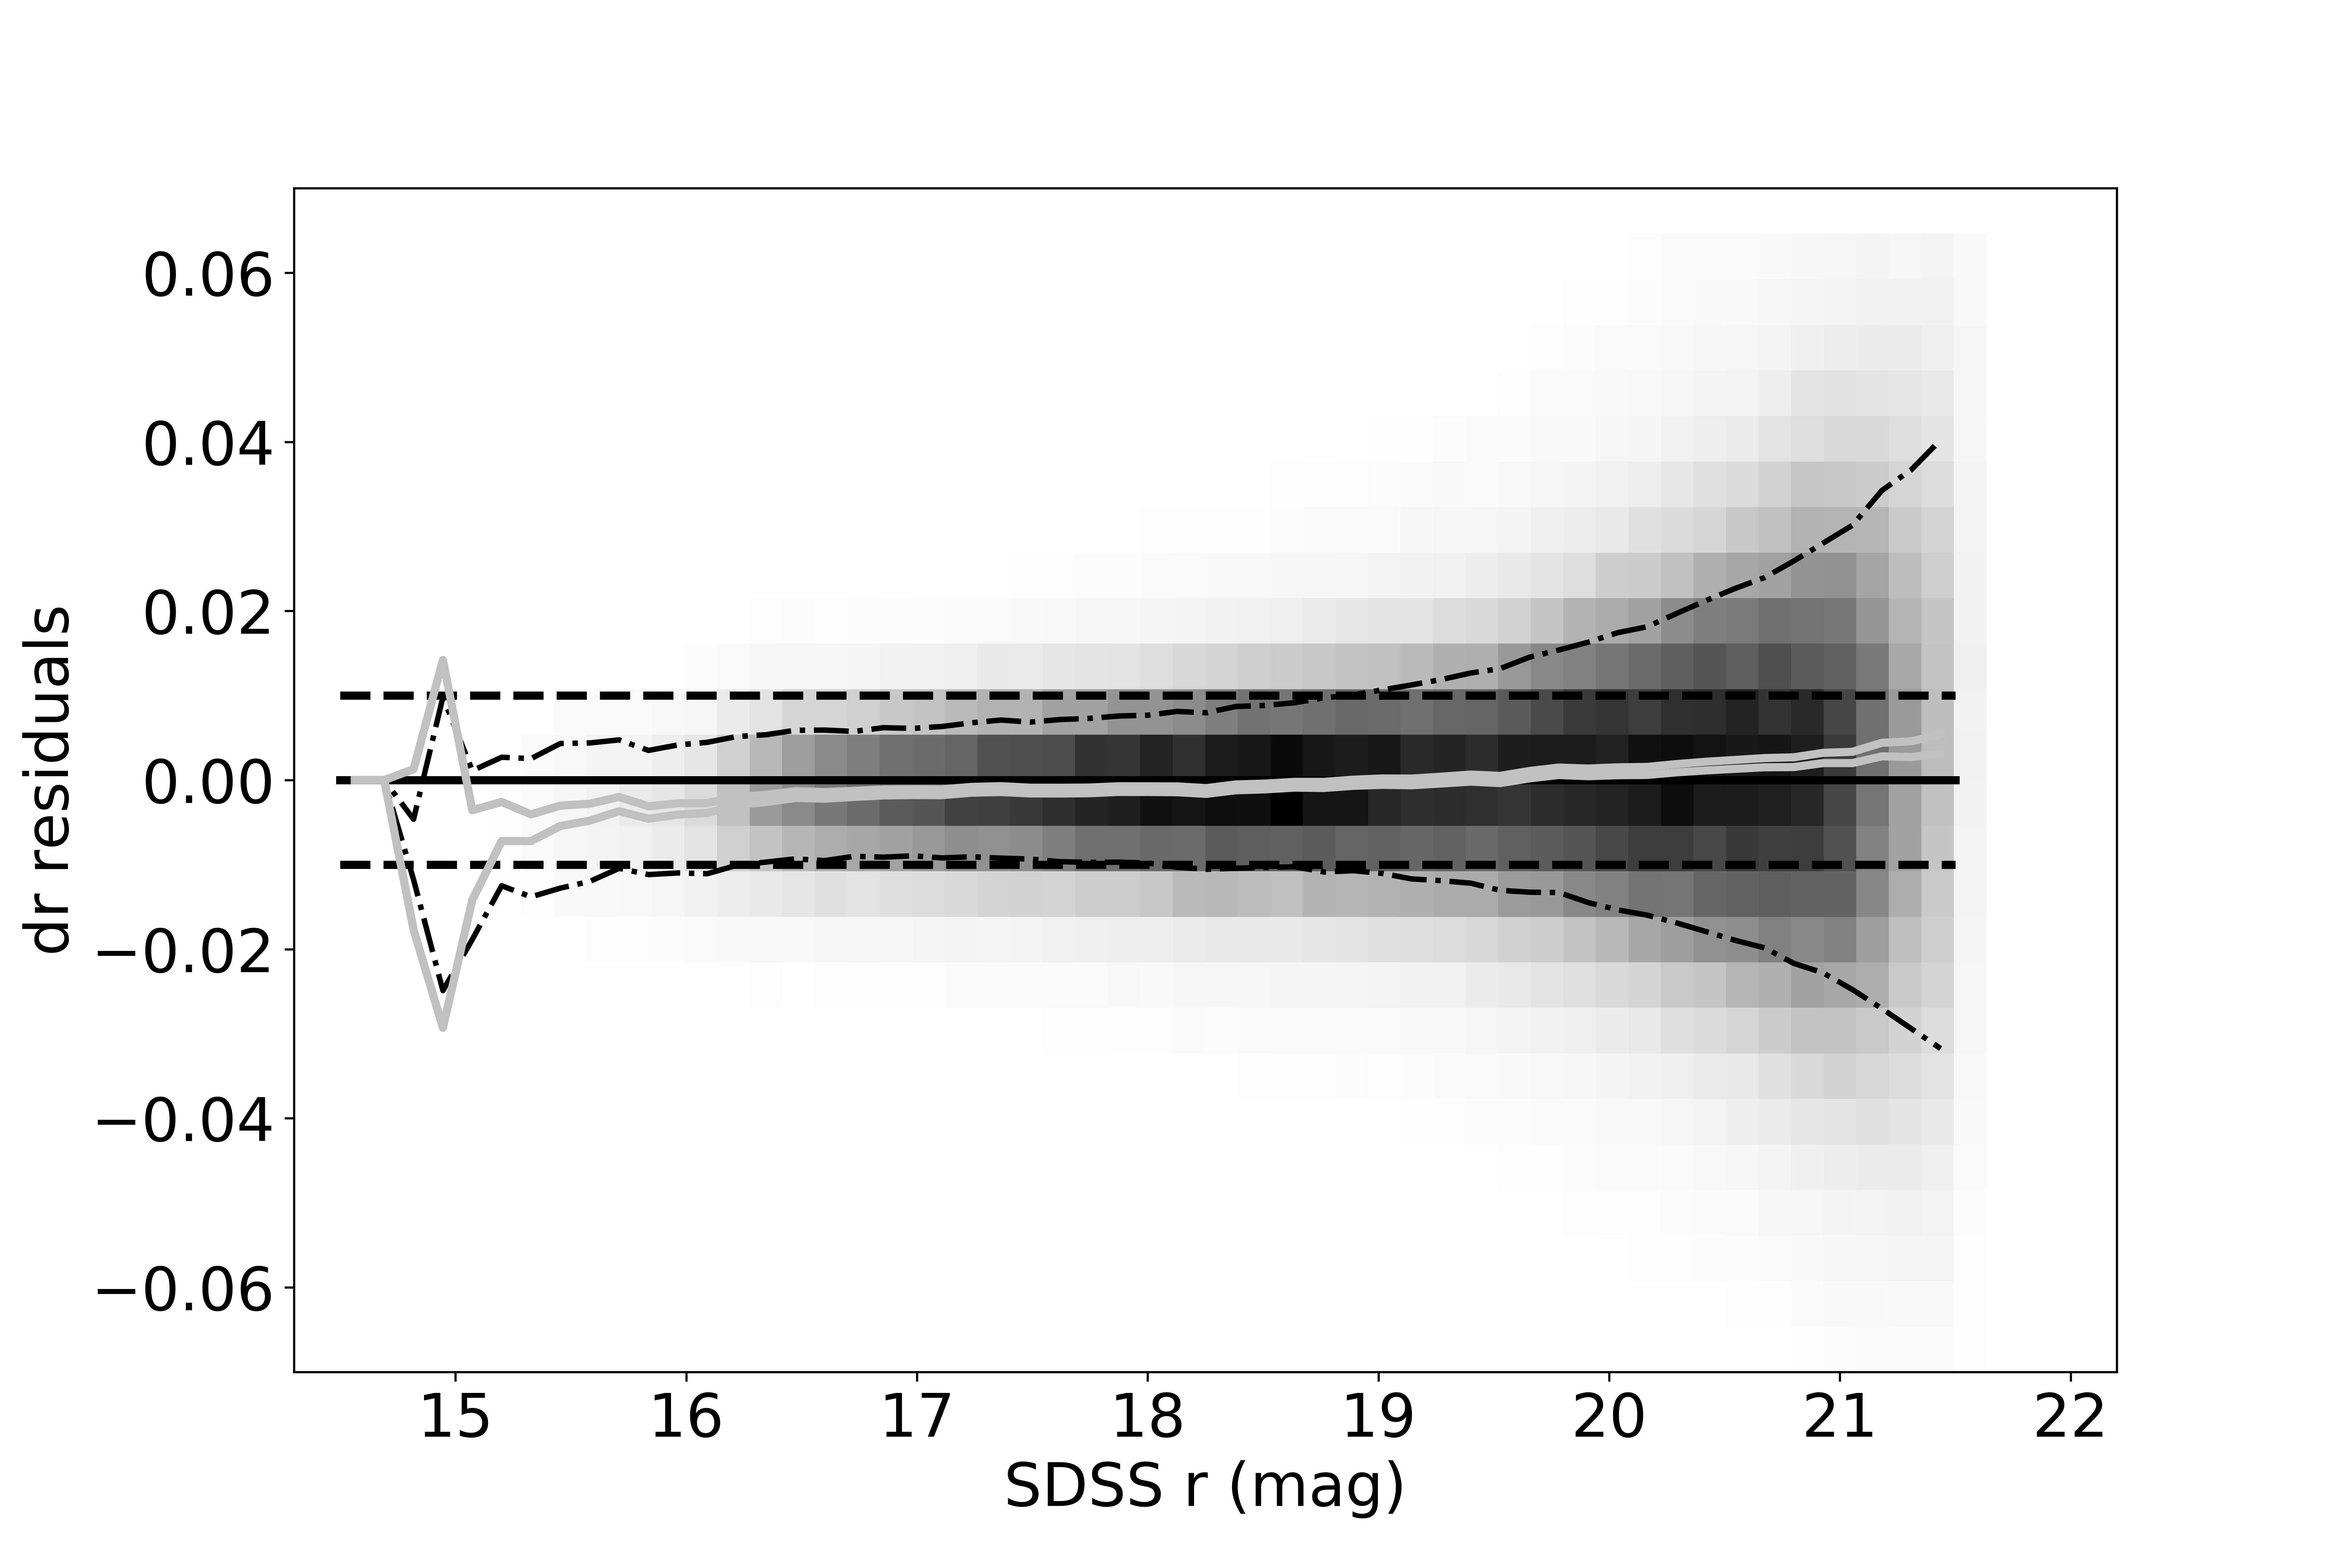
\includegraphics[width=7cm]{figures/colorResidDES2_dr_rmag_Hess.png}
    \centering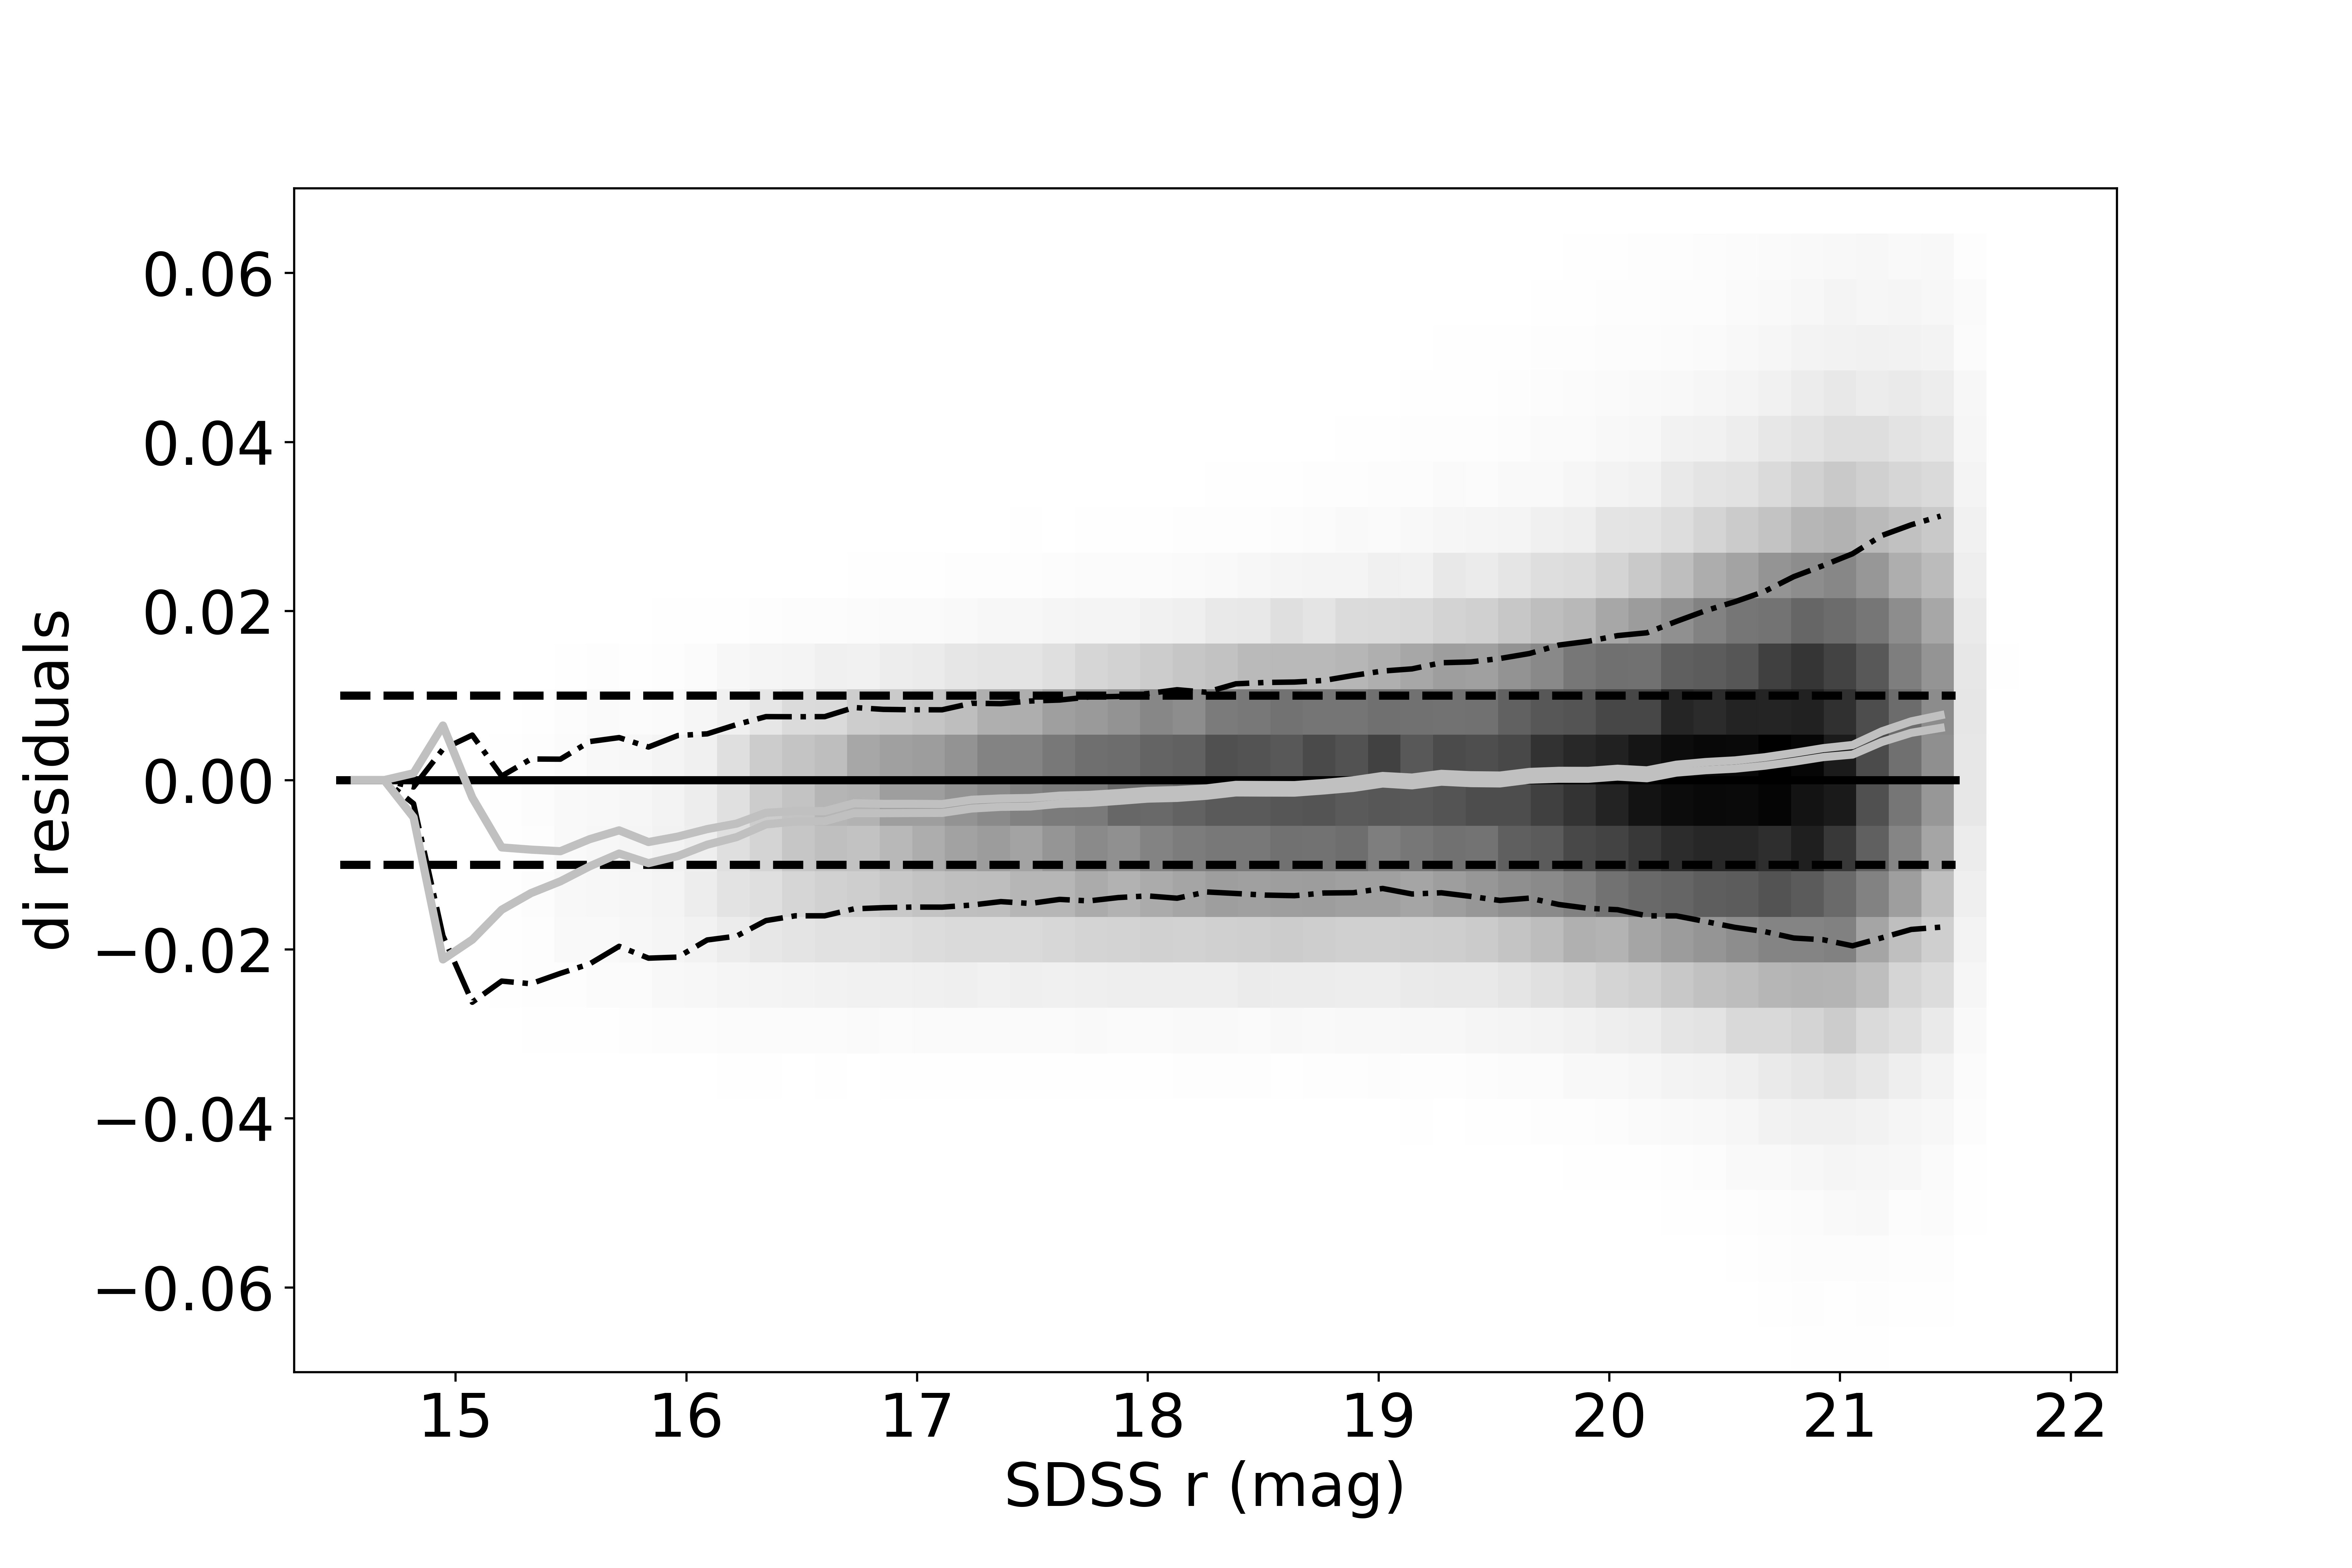
\includegraphics[width=7cm]{figures/colorResidDES2_di_rmag_Hess.png} 
\caption{A comparison of the magnitude differences between the SDSS v3.4 catalog
and DES catalog, for the $r$ and $i$ bands. Note the good agreement even at the
faint end ($20<r<21$), where Gaia Gmag magnitudes appear too faint by about
0.02 mag (see Figure~\ref{fig:gaiaJump}).} 
\label{fig:drVSr}
\end{figure}



\subsection{Comparison of the new v3.4 SDSS catalog and $u$ band data from the CFIS catalog  \label{sec:CFIStest}} 

The comparison of the new SDSS catalog with the DES and Pan-STARRS catalogs in the previous
section did not include the $u$ band. To assess the quality of $u$ band zeropoint calibration, 
we use the CFIS catalog (see Section~\ref{ssec:cfis}). The CFIS $u$ band photometry was 
calibrated using a combination of the SDSS, Pan-STARRS and GALEX UV data. Given that
we recalibrated the new SDSS catalog using Gaia data, for this comparison it shouldn't 
matter that SDSS data were used in calibration of the CFIS catalog. Nevertheless, the
results of this section should be treated with caution. 

A star-by-star comparison for about 150,000 sufficiently bright blue stars is illustrated in 
Figure~\ref{fig:CFIS}. The binned median scatter for Declination direction is 5.7 millimag with 
systematic differences of up to about 0.01 mag. The constraints in R.A. direction are more noisy, 
with residuals appearing about twice as large as in Declination direction. 
 
\begin{figure}[th!]
    \centering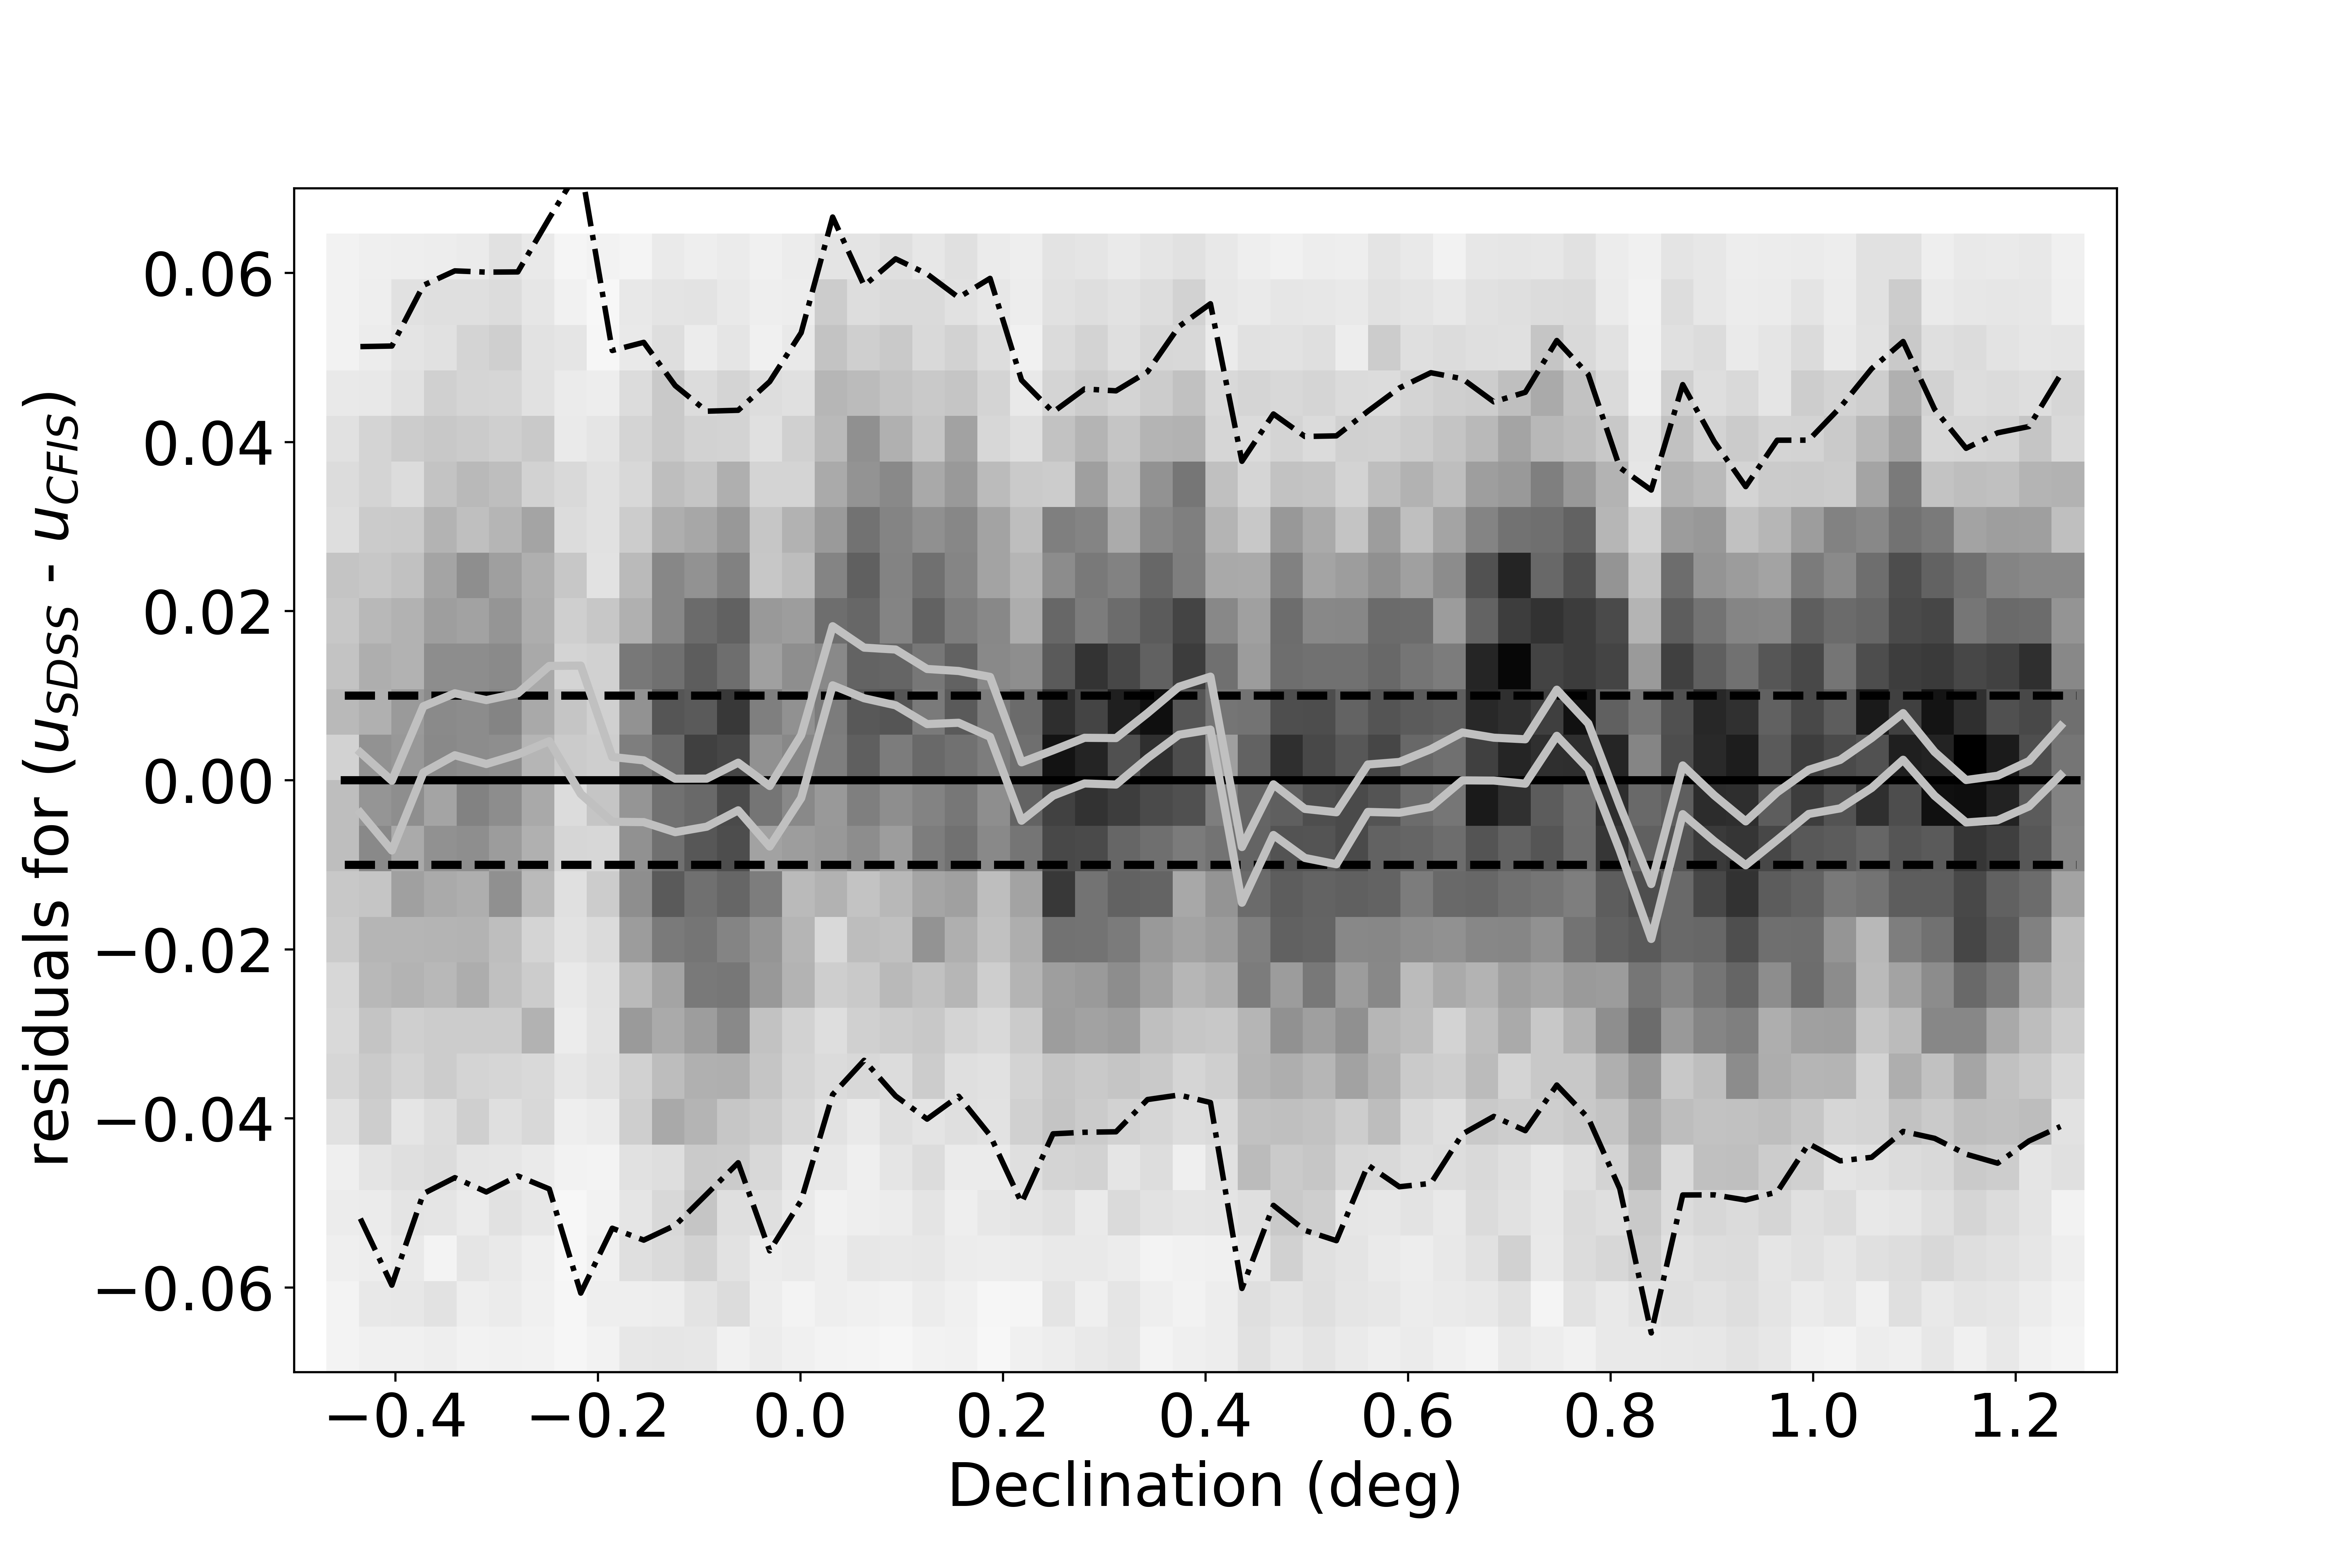
\includegraphics[width=9cm]{figures/colorResidCFISug_Dec_Hess.png} 
\caption{Analogous to Figure~\ref{fig:graycorrDec}, except that here residuals 
between the SDSS $u$ band magnitudes and $u$ band magnitudes from the CFIS
catalog (corrected for small color terms, $\sim0.05$ mag, as a function of the $u-g$ color),
for $\sim$150,000 matched stars with $1.0 <u-g < 2.1$ and $r<20$ are shown. 
The binned median scatter is 5.7 millimag. Note that the CFIS data are available
only for Declination $>$ -0.45 degree.}
\label{fig:CFIS}
\end{figure}

\subsection{Offsets from AB magnitude scale \label{sec:AB}} 






\section{Discussion and Conclusions} \label{sec:disc}

To enable further progress in cosmological and other high-precision photometric measurements, 
modern multi-band photometric sky surveys aim to deliver measurements accurate at the 1\% 
(0.01 mag) level. Over the last decade a number of such large-scale surveys approached, and
often exceeded this photometric accuracy threshold. For ground-based surveys, that are 
affected by variable atmospheric effects and hardware responses to changes in local environment
(e.g. temperature), significant improvements can be achieved by averaging multiple observations. 

In this paper, we have described the construction and tests of an updated version of the so-called
SDSS Stripe 82 Standard Star catalog \citep{Ivez07} that lists averaged SDSS photometry for about
a million non-variable stars. Additional post-2007 SDSS data include about 
2-3 times more measurements per star than in the original catalog, resulting in 1.4-1.7 times smaller 
random photometric errors (precision) than in the original catalog, and about three times as small 
as for individual SDSS runs.

Thanks to the availability of photometric data from recent wide-field surveys (Gaia, DES, Pan-STARRS
and CFIS), we were able to derive robust zeropoint corrections and establish that this new catalog
is superior to the original catalog. Using a combination of comparison to other catalogs and 
astrophysical constraints, we find that that the contribution of the zeropoint errors to photometric
errors is $<5$ millimag for the $gri$ bands, and $<10$ millimag for the $u$ and $z$ bands. 

Various catalog cross-comparisons have revealed minor problems with all the analyzed catalogs.
For example, we detected DES $z$ band zeropoint errors of up to 0.01-0.02 mag, as a function 
of R.A., and demonstreted that Gaia Gmag magnitudes appear too faint by about 0.02 mag at
Gmag$\sim$20.
 
XXX We constrained offsets from the absolute AB magnitude scale using three stars with 
the HST CalSpec absolute photometry data. The estimated AB zeropoint offsets in the $ugriz$ bands
are equal to..., respectively. XXX

Thanks to its high stellar density, about 1 star per square arcmin, and demonstrated sub-percent 
photometry, this catalog is a good resource for both calibrating and testing other surveys. In
particular, it will enable high-precision photometric testing of data collected during the 
commissioning phase of the Rubin Observatory Legacy Survey of Space and Time. 
  

\acknowledgments
Funding for the SDSS and SDSS-II has been provided by the Alfred P. Sloan Foundation, the Participating
Institutions, the National Science Foundation, the US Department of Energy, the National Aeronautics and 
Space Administration, the Japanese Monbukagakusho, the Max Planck Society, and the Higher Education 
Funding Council for England. The SDSS Web site is http://www.sdss.org.
 
\vspace{5mm}
\facilities{SDSS, Pan-STARRS, DECam, CFHT}

\software{numpy \citep{numpy}, matplotlib \citep{matplotlib}, scipy \citep{scipy}, 
       astropy \citep{astropy-1, astropy-2}, astroML \citep{2012cidu.conf...47V}.}

%%%%%%%%%%%%%%%%%%%%%
%% BIBLIOGRAPHY
\bibliography{S82SSC}{}
\bibliographystyle{aasjournal}

%\appendix
%\section{Appendix information}
%
%Here is Appendix A.
 
\end{document}
 




name     &     R.A. (deg)    &      Dec (deg)       &     $V$   &     $B-V$   &   
  GD50  &    57.209108    &    $-$0.975636   &   14.06  &  $-$0.28   &  13.409  & 13.784 & 13.784 & 14.6545  & $-$9999  \\ 

                                                                                                 A$_r$ 
                                                                                          &  0.513    &  13.376  & 13.816 & 14.279 & 14.649 & 15.002  






GAP? 
lds749b   323.067638   0.254000 14.463  14.550  14.8037  15.0312  15.2784

